\documentclass[10pt,prd,aps,nobibnotes,superscriptaddress,preprintnumbers,notitlepage]{revtex4-1}

\bibliographystyle{apsrev4-1}
\setlength{\topmargin}{-14mm}
\usepackage{graphicx,bm,braket,amsmath}
\graphicspath{{./images/}}
\usepackage{amssymb}
\usepackage{xfrac}
\usepackage{mathrsfs}
\usepackage{cancel}
\usepackage{booktabs}
\usepackage{longtable}
\usepackage{xcolor}
\usepackage{comment}
% hyperref must be loaded last so it can patch the other packages cleanly.
\usepackage{hyperref}

\hypersetup{
  colorlinks=true,
  linkcolor=blue!60!black,
  citecolor=blue!60!black,
  urlcolor=blue!60!black
}

\def \ul{\underline}
\def \vp{\varphi}
\def \ds{\displaystyle}
\def \pa{\partial}

\newcommand{\rb}{\rho_{\rm B}}
\newcommand{\extra}{\rho_{\rm extra}}
\newcommand{\ep}{e_{ij}^+}
\newcommand{\ec}{e_{ij}^\times}
\newcommand{\khat}{\hat{k}}
\newcommand{\Omgw}{\Omega_{\rm GW}}
\newcommand{\Agw}{\mathcal{A}_{\rm GW}}
\newcommand{\n}{\hat{n}}
\newcommand{\vhat}{\hat{v}}
\newcommand{\p}{\hat{p}}
\newcommand{\z}{\hat{z}}
\newcommand{\x}{\hat{x}}
\newcommand{\y}{\hat{y}}
\newcommand{\that}{\hat{\theta}}
\newcommand{\ph}{\hat{\phi}}
\newcommand{\rhat}{\hat{r}}
\newcommand{\xb}{{\bf x}}
\newcommand{\br}{{\bf r}}
\newcommand{\bq}{{\bf q}}
\newcommand{\bp}{{\bf p}}
\newcommand{\kb}{{\bf k}}
\newcommand{\bxi}{{\boldsymbol{\xi}}}
\newcommand{\ub}{{\bf u}}
\newcommand{\tf}{\tilde{f}}

\begin{document}
\title{Polarization of Gravitational Waves From Turbulence:
       Tension Between Simulation and Analytic Approaches}
\date{\today}

\author{Titus Brock}
\email{tbrock@andrew.cmu.edu}
\affiliation{McWilliams Center for Cosmology and Department of Physics,
Carnegie Mellon University, Pittsburgh, PA 15213, USA}

\author{Murman Gurgenidze}
\email{mgurgeni@andrew.cmu.edu}
\affiliation{McWilliams Center for Cosmology and Department of Physics,
Carnegie Mellon University, Pittsburgh, PA 15213, USA}

\author{Tina Kahniashvili}
\email{tinatin@andrew.cmu.edu}
\affiliation{McWilliams Center for Cosmology and Department of Physics,
Carnegie Mellon University, Pittsburgh, PA 15213, USA}
\affiliation{School of Natural Sciences and Medicine, Ilia State University, 0194 Tbilisi, Georgia}
\affiliation{Abastumani Astrophysical Observatory, Tbilisi, GE-0179, Georgia}


\maketitle

\tableofcontents

\section{Gravitational waves from a turbulent source}
\label{sec:framework}

Before specializing to particular spectral and temporal models, we collect the
standard analytic derivation of the gravitational-wave (GW) spectrum sourced by
turbulence \cite{2002Kosowsky,2007Gogoberidze,2008Kahniashvili,Caprini:2018mtu,2007Maggiore}.
This fixes the conventions used throughout and, in particular, shows why the
remaining sections reduce the problem to computing the contracted source
correlator $H_{ijij}(\kb,\omega)$ of Eq.~\eqref{eq: main} on the diagonal
$\omega=k$.

\subsection{Sourced wave equation}
\label{sec:framework-waveeq}

Write the tensor perturbations of a spatially flat FLRW background as
\begin{equation}
  ds^2 = a^2(\tau)\bigl[-d\tau^2 + (\delta_{ij}+h_{ij})\,dx^i dx^j\bigr],
  \qquad \pa_i h_{ij}=h_{ii}=0,
  \label{eq:metric-tt}
\end{equation}
with $h_{ij}$ transverse-traceless (TT). The linearized Einstein equations give
\begin{equation}
  h_{ij}'' + 2\frac{a'}{a}\,h_{ij}' - \nabla^2 h_{ij}
  = 16\pi G\,a^2\,\Pi_{ij}^{\rm TT},
  \label{eq:gw-wave}
\end{equation}
where $' = d/d\tau$ and $\Pi_{ij}^{\rm TT}$ is the TT part of the anisotropic
stress. For an incompressible, non-relativistic turbulent fluid the source is
the Reynolds stress,
\begin{equation}
  \Pi_{ij}^{\rm TT}(\kb,\tau) = \Lambda_{ij,lm}(\khat)\,T_{lm}(\kb,\tau),
  \qquad
  T_{lm} = w\,v_l v_m,
  \qquad
  \Lambda_{ij,lm} = P_{il}P_{jm}-\tfrac12 P_{ij}P_{lm},
  \label{eq:source-tt}
\end{equation}
with $w=\bar\rho+\bar p$ the enthalpy density, $P_{ij}=\delta_{ij}-\khat_i\khat_j$,
and $\Lambda$ the TT projector. The double TT projection together with the
Gaussian (Wick) reduction of the quartic velocity correlator collapses the
two-point function of \eqref{eq:source-tt} onto the contracted form
$R_{ijij}=R_{ii}R_{jj}+\tfrac13 R_{ij}R_{ij}$ that appears in Eq.~\eqref{eq: main}.

Turbulence acts on eddy-turnover times short compared with a Hubble time, so
over the source lifetime we drop the expansion ($a\approx 1$, friction
negligible) and Eq.~\eqref{eq:gw-wave} becomes, in Fourier space, a forced
oscillator,
\begin{equation}
  h_{ij}''(\kb,\tau) + k^2 h_{ij}(\kb,\tau) = 16\pi G\,\Pi_{ij}^{\rm TT}(\kb,\tau).
  \label{eq:gw-osc}
\end{equation}

\subsection{Green-function solution and the GW spectrum}
\label{sec:framework-green}

The retarded solution of Eq.~\eqref{eq:gw-osc} and its time derivative are
\begin{equation}
  h_{ij}(\kb,\tau) = \frac{16\pi G}{k}\!\int_{\tau_i}^{\tau}\!d\tau'\,
  \sin[k(\tau-\tau')]\,\Pi_{ij}^{\rm TT}(\kb,\tau'),
  \qquad
  \dot h_{ij}(\kb,\tau) = 16\pi G\!\int_{\tau_i}^{\tau}\!d\tau'\,
  \cos[k(\tau-\tau')]\,\Pi_{ij}^{\rm TT}(\kb,\tau').
  \label{eq:greens}
\end{equation}
With the Isaacson energy density $\rho_{\rm GW}=\langle\dot h_{ij}\dot h_{ij}\rangle/(32\pi G)$
and the unequal-time correlator (UETC) of the TT stress,
\begin{equation}
  \langle\Pi_{ij}^{\rm TT}(\kb,\tau_1)\,\Pi_{ij}^{\rm TT*}(\kb',\tau_2)\rangle
  = (2\pi)^3\,\delta^{(3)}(\kb-\kb')\,\Pi(k;\tau_1,\tau_2),
  \label{eq:uetc}
\end{equation}
inserting \eqref{eq:greens} and averaging the product
$\cos[k(\tau-\tau_1)]\cos[k(\tau-\tau_2)]\to\tfrac12\cos[k(\tau_1-\tau_2)]$ over
the fast GW oscillations gives the master formula
\begin{equation}
  \frac{d\rho_{\rm GW}}{d\ln k}
  \simeq \frac{2G\,k^3}{\pi}\!\int\! d\tau_1\!\int\! d\tau_2\,
  \cos[k(\tau_1-\tau_2)]\,\Pi(k;\tau_1,\tau_2).
  \label{eq:master}
\end{equation}
The GW spectrum is thus the temporal Fourier transform of the source UETC,
evaluated at the on-shell frequency $\omega=k$. For a statistically stationary
(or quasi-stationary) source, $\Pi(k;\tau_1,\tau_2)=\Pi(k;\tau_1-\tau_2)$ and the
double time integral factorizes into the source duration $T_{\rm src}$ times the
temporal transform $\widetilde\Pi(k,\omega)=\int d(\Delta\tau)\,e^{i\omega\Delta\tau}\Pi(k;\Delta\tau)$,
which is precisely the spatio-temporal correlator $H_{ijij}(\kb,\omega)$ of
Eq.~\eqref{eq: main}. Hence
\begin{equation}
  \frac{d\rho_{\rm GW}}{d\ln k} \;\propto\; k^3\,H_{ijij}(\kb,\omega)\big|_{\omega=k}
  \quad\Longrightarrow\quad
  \Omega_{\rm GW}(p)\;\propto\; p^3\,H(p,p),
  \qquad p=\frac{k}{k_0},\ \ q=\frac{\omega}{k_0},
  \label{eq:omega-diag}
\end{equation}
the GW dispersion $\omega=k$ becoming the diagonal $q=p$ used in
Sec.~\ref{sec:spectrum-survey} (with characteristic strain
$h_c^2(p)=p\,H(p,p)$). Everything downstream is therefore an evaluation of
$H_{ijij}$, whose spatial part is a convolution of the velocity power spectrum
(quadratic source, Eqs.~\eqref{eq: H-after-r}--\eqref{eq: H-convolution}) and
whose temporal part is the decorrelation model carried by $\Pi(k;\tau_1,\tau_2)$.

\subsection{Spectral shape from the literature}
\label{sec:framework-shape}

For Kolmogorov inertial-range input the analytic results have three robust
pieces:
\begin{itemize}
  \item \emph{Infrared ($k\ll k_0$):} causality forces the stress correlator to
  be analytic (white) as $k\to0$, so $H\to\text{const}$ and
  $\Omega_{\rm GW}\propto k^3$ \cite{Caprini:2018mtu,2008Kahniashvili}.
  \item \emph{Peak ($k\sim k_0$):} set by the largest eddies, with parametric
  amplitude $(d\Omega_{\rm GW}/d\ln k)_{\rm peak}\sim (H_\ast/k_0)\,\Omega_K^2$,
  i.e.\ the squared kinetic-energy fraction suppressed by the source-duration
  factor $H_\ast/k_0\sim H_\ast\tau_{\rm eddy}$ \cite{2002Kosowsky,2008Kahniashvili}.
  \item \emph{Ultraviolet ($k\gg k_0$):} \emph{model-dependent}, fixed by the
  temporal decorrelation $\Pi(k;\tau_1,\tau_2)$. Kraichnan sweeping gives the
  Gogoberidze tail \cite{2007Gogoberidze}, while a $\delta$-correlated or a
  decaying-turbulence kernel give different slopes.
\end{itemize}
The UV slope is precisely where the four UETC models derived below
($\delta$-spectrum vs.\ white-noise, Kraichnan vs.\ decay) differ, which is the
focus of the remainder of the paper.

\subsection{The model space, and a uniform notation for the kernels}
\label{sec:model-space}

Every kernel derived in this paper is a choice of two independent ingredients,
and it is worth making the factorisation explicit at the outset because most of
the disagreements in the literature---and every discrepancy discussed below---trace
to one axis or the other rather than to the derivation itself.

\paragraph{Axis 1: the spatial source model $S$.} What the fluid two-point
function is taken to be. We use four:
\begin{itemize}\itemsep0pt
  \item $S_{\rm K41}$: Kolmogorov inertial range, $E(k)\propto k^{-5/3}$ on
    $k_0<k<k_d$, with $R=(k_d/k_0)^{4/3}$ the Reynolds number
    (Sec.~\ref{sec:kraichnan-k41});
  \item $S_{\delta k}$: monochromatic, $E(k)=E_0\delta(k-k_0)$
    (Sec.~\ref{sec:delta-k});
  \item $S_{\delta r}$: real-space white noise, $R_{ij}\propto\delta^{(3)}(\br)$,
    equivalently $E(k)\propto k^{2}$ (Sec.~\ref{sec:white});
  \item $S_{\rm full}$: a full input spectrum---a Batchelor or Saffman infrared
    band joined to the Kolmogorov inertial range (Sec.~\ref{sec:omega-over-k}).
\end{itemize}

\paragraph{Axis 2: the temporal model $T$.} What the unequal-time correlator
(UETC) of the source is taken to be. We use four:
\begin{itemize}\itemsep0pt
  \item $T_{\rm sw}$: Kraichnan sweeping, a \emph{Gaussian} in the time
    difference, $f(\tau)=\exp(-\tfrac{\pi}{4}\eta_k^2\tau^2)$ with
    $\eta_k\propto\varepsilon^{1/3}k^{2/3}$;
  \item $T_{\rm dec}$: BK2016 decaying turbulence, a \emph{power law}
    $f(\tau)=(1+|\tau|/\tau_k)^{-2/3}$;
  \item $T_{\rm imp}$: impulsive, $\delta$-correlated in time
    (Sec.~\ref{sec:impulsive});
  \item $T_{\rm burst}$: a source of finite duration $\Delta t$
    (Sec.~\ref{sec:burst}).
\end{itemize}

\paragraph{Notation.} We write the resulting dimensionless kernel as
\begin{equation}
  H[S,T](p,q;M,R),
  \qquad p=\frac{k}{k_0},\quad q=\frac{\omega}{k_0},
  \label{eq:kernel-notation}
\end{equation}
suppressing $M$ or $R$ where the kernel does not depend on them, and the GW
spectrum on the sound-cone diagonal is always
$\Omega_{\rm GW}(p)\propto p^{3}H[S,T](p,p)$. Table~\ref{tab:model-grid} lists
every combination derived here, its defining equation, and its analytic
structure; Sec.~\ref{sec:model-differences} then compares them systematically.
Two entries of the grid deserve a warning before any spectrum is read off them:
$S_{\delta k}$ has zero spectral width and $S_{\delta r}$ has no infrared power
at all, so both violate the hypotheses of the universal infrared theorem
(Sec.~\ref{sec:cps-reproduction}) and neither should be expected to show $k^{3}$.

\begin{table*}[ht]
  \centering
  \begin{tabular}{llll}
  \hline
  Kernel & Defining equation & Analytic structure & Sec. \\
  \hline
  $H[S_{\rm K41},T_{\rm sw}]$   & Eq.~\eqref{eq:Hijij-AppA-dimless}
    & 2-D wavevector integral, Gaussian temporal factor & \ref{sec:kraichnan-k41} \\
  $H[S_{\rm K41},T_{\rm dec}]$  & Eq.~\eqref{eq:ft-of-product}
    & 2-D wavevector $\times$ 1-D Feynman parameter & \ref{sec:decaying-peak} \\
  $H[S_{\delta k},T_{\rm sw}]$  & Eq.~\eqref{eq:dimless-delta-Kraichnan}
    & closed form; $M$ in the frequency scale only & \ref{sec:delta-kraichnan} \\
  $H[S_{\delta k},T_{\rm dec}]$ & Eq.~\eqref{eq:dimless-delta-decay}
    & closed form, Eq.~\eqref{eq:conv-equals-cosT} & \ref{sec:delta-decay} \\
  $H[S_{\delta r},T_{\rm sw}]$  & Eq.~\eqref{eq:dimless-white-Kraichnan}
    & 2-D wavevector integral; $M$-cutoff in the bounds & \ref{sec:white} \\
  $H[S_{\delta r},T_{\rm dec}]$ & Eq.~\eqref{eq:dimless-white-decay}
    & 2-D wavevector $\times$ Eq.~\eqref{eq:two-scale-feynman} & \ref{sec:white} \\
  $H[S_{\delta k},T_{\rm imp}]$ & Eq.~\eqref{eq:dimless-impulsive}
    & closed form; no $M$ or $q$ dependence & \ref{sec:impulsive} \\
  $H[S_{\delta k},T_{\rm burst}]$ & Eq.~\eqref{eq:rs2-spectrum-dt}
    & closed form; window factor $\sin^{2}$ & \ref{sec:burst} \\
  $H[S_{\rm full},T_{\rm sw}]$  & Eq.~\eqref{eq:full-input-spectrum}
    & as $S_{\rm K41}$ with a shape factor $S(k)$ & \ref{sec:omega-over-k} \\
  \hline
  \end{tabular}
  \caption{The model grid. Each kernel is a (spatial source, temporal UETC)
  pair in the notation of Eq.~\eqref{eq:kernel-notation}. The analytic structure
  column is what actually has to be evaluated: note that the two decaying
  entries are closed-form or single-integral rather than the frequency
  convolutions they are usually written as, by
  Eqs.~\eqref{eq:conv-equals-cosT} and \eqref{eq:two-scale-feynman}.}
  \label{tab:model-grid}
\end{table*}

\section{Kraichnan--K41 Model (Gogoberidze 2007)}
\label{sec:kraichnan-k41}

We use the spatial/temporal Fourier pair $R_{ij}(\br,\tau) = \int \tfrac{d^3k}{(2\pi)^3}e^{i\kb\cdot\br}F_{ij}(\kb,\tau)$ and $f(\eta_k,\tau)=\int\tfrac{d\omega}{2\pi}e^{-i\omega\tau}\tf(\eta_k,\omega)$, and adopt the isotropic incompressible model of \cite{2007Gogoberidze} (Eqs.~23--26),
\begin{equation}
  F_{ij}(\kb,\tau) = A(k)\,P_{ij}(\khat)\,f(\eta_k,\tau),
  \qquad
  P_{ij}(\khat)=\delta_{ij}-\khat_i\khat_j,
  \label{eq:Fij-iso}
\end{equation}
with $A(k)=C_k\epsilon^{2/3}k^{-11/3}/4\pi$, $f(\eta_k,\tau)=\exp(-\tfrac{\pi}{4}\eta_k^2\tau^2)$, and $\eta_k=\tfrac{1}{\sqrt{2\pi}}\epsilon^{1/3}k^{2/3}$.

The fourth-rank Fourier-space correlator
$H_{ijkl}(\kb,\omega)=(2\pi)^{-4}\!\int d\tau\,d^3\bxi\,e^{i\omega\tau-i\kb\cdot\bxi}R_{ijkl}(\bxi,\tau)$ with the contraction
$R_{ijij}=R_{ii}R_{jj}+\tfrac{1}{3}R_{ij}R_{ij}$ (Gogoberidze Eq.~28) reads, in real space,
\begin{equation}
  H_{ijij}(\kb,\omega) = \frac{1}{(2\pi)^4}\!\int d\tau\,d^3\br\,e^{i\omega\tau-i\kb\cdot\br}
  \Bigl[R_{ii}(\br,\tau)R_{jj}(\br,\tau)+\tfrac{1}{3}R_{ij}(\br,\tau)R_{ij}(\br,\tau)\Bigr].
  \label{eq: main}
\end{equation}
Inserting the spatial Fourier representation of $R_{ij}$, the $\br$ integral produces a momentum-conserving $\delta^{(3)}(\kb-\bq-\bp)$. Renaming $\bq\to\kb_1$, $\ub=\kb-\kb_1$,
\begin{equation}
  H_{ijij}(\kb,\omega) = \frac{1}{(2\pi)^7}\!\int d\tau\,e^{i\omega\tau}\,
  d^3k_1\!\left[F_{ii}(\kb_1,\tau)F_{jj}(\ub,\tau)+\tfrac{1}{3}F_{ij}(\kb_1,\tau)F_{ij}(\ub,\tau)\right].
  \label{eq: H-after-r}
\end{equation}
The temporal Fourier transform then converts the $\tau$ integral into a frequency $\delta$-function, leaving the frequency convolution
\begin{equation}
  H_{ijij}(\kb,\omega) = \frac{1}{(2\pi)^8}\!\int d^3k_1\,d\omega_1
  \left[\tilde F_{ii}(\kb_1,\omega_1)\tilde F_{jj}(\ub,\omega-\omega_1)
  +\tfrac{1}{3}\tilde F_{ij}(\kb_1,\omega_1)\tilde F_{ij}(\ub,\omega-\omega_1)\right].
  \label{eq: H-convolution}
\end{equation}

Substituting Eq.~\eqref{eq:Fij-iso} and using $P_{ii}(\khat)=2$ together with $P_{ij}(\khat_1)P_{ij}(\hat u)=1+(\khat_1\cdot\hat u)^2$, the tensor contractions reduce Eq.~\eqref{eq: H-convolution} to
\begin{equation}
  H_{ijij}(\kb,\omega) = \frac{1}{(2\pi)^8}\!\int d^3k_1\,d\omega_1\,
  A(k_1)A(u)\,\tf(\eta_{k_1},\omega_1)\tf(\eta_u,\omega-\omega_1)
  \left[4+\tfrac{1}{3}\bigl(1+(\khat_1\cdot\hat u)^2\bigr)\right].
  \label{eq: H-with-P}
\end{equation}
This is the Fourier representation valid for all $k$; we treat $\kb > \kb_0$ and $\kb \leq \kb_0$ separately below.

\subsection{\texorpdfstring{$\kb > \kb_0$}{k > k0}}

The law of cosines $\khat_1\cdot\hat u = (k^2-k_1^2-u^2)/(2k_1 u)$ turns the bracket in Eq.~\eqref{eq: H-with-P} into a homogeneous polynomial in $(k,k_1,u)$; expanding and grouping gives the geometric kernel
\begin{equation}
  \mathcal{K}(k,k_1,u)\equiv \frac{27}{6}+\frac{k^4}{12k_1^2u^2}+\frac{k_1^2}{12u^2}+\frac{u^2}{12k_1^2}
  -\frac{k^2}{6u^2}-\frac{k^2}{6k_1^2}
  \qquad (\text{cf.\ Eq.~29 of \cite{2007Gogoberidze}}).
  \label{eq: K-kernel}
\end{equation}
The temporal transform $\tf(\eta_k,\omega) = (2/\eta_k)\exp(-\omega^2/\pi\eta_k^2)$ combines with $A(k)$ into the single spectral factor
\begin{equation}
  g(k,\omega) \equiv A(k)\,\tf(\eta_k,\omega) = \frac{2E_k}{4\pi k^2\eta_k}\exp\!\left(-\frac{\omega^2}{\pi\eta_k^2}\right),
  \qquad E_k = C_k\epsilon^{2/3}k^{-5/3}.
  \label{eq: g-def}
\end{equation}
Going to spherical coordinates for $\kb_1$ ($d^3k_1 = k_1^2\,dk_1\,d\phi\,d\mu$ with $\mu=\hat\kb\cdot\hat\kb_1$), the azimuthal integral contributes $2\pi$. Trading $\mu$ for $u=\sqrt{k^2+k_1^2-2kk_1\mu}$ via $d\mu = u\,du/(k k_1)$, with $u\in[|k-k_1|,k+k_1]$,
\begin{equation}
  H_{ijij}(\kb,\omega) = \frac{1}{(2\pi)^7}\!\int_0^\infty\!\frac{k_1\,dk_1}{k}\int_{|k-k_1|}^{k+k_1}\!u\,du\int_{-\infty}^\infty\! d\omega_1\,
  g(k_1,\omega_1)\,g(u,\omega-\omega_1)\,\mathcal K(k,k_1,u).
  \label{eq: conversion}
\end{equation}

Switching to the dimensionless variables $q=k_1/k$, $s=u/k$, $\Omega=\omega/(\epsilon^{1/3}k^{2/3})$, $\Omega_1=\omega_1/(\epsilon^{1/3}k^{2/3})$, $g$ becomes $g(k,\omega)=(1/\sqrt{2\pi})\,C_k\epsilon^{1/3}k^{-13/3}\exp(-2\Omega^2)$. The product $g(k_1,\omega_1)g(u,\omega-\omega_1)$ thus separates into a dimensional prefactor $\propto k^{-26/3}$ times a manifestly dimensionless Gaussian envelope $\Phi(q,\Omega_1;s,\Omega-\Omega_1) = q^{-13/3}s^{-13/3}\exp[-2\Omega_1^2q^{-4/3}-2(\Omega-\Omega_1)^2s^{-4/3}]$. Collecting all $k$-dependent factors gives the scaling form
\begin{equation}
  H_{ijij}(\kb,\omega) = \frac{C_k^2\,\epsilon}{256\,\pi^8}\,k^{-5}\,\mathfrak H(\Omega),
  \qquad
  \mathfrak H(\Omega) = \int_0^\infty\!dq\,q\int_{-\infty}^\infty\!d\Omega_1\int_{|1-q|}^{1+q}\!ds\,s\;\Phi\,\widetilde{\mathcal K}(q,s),
  \label{eq: H-compact}
\end{equation}
with $\widetilde{\mathcal K}(q,s)=\mathcal K(k,k_1,u)|_{k_1=qk,u=sk}$ (homogeneous of degree zero). All physical scales are absorbed in the prefactor $C_k^2\epsilon k^{-5}$.

\subsection{Gogoberidze (2007) Appendix~A form}

Using the Gaussian-erfc identity (Eq.~A.1 of \cite{2007Gogoberidze}, $\int_0^\infty dy\,e^{-Ay^2-B(y-x)^2}=\sqrt{\pi/[4(A+B)]}\,e^{-ABx^2/(A+B)}\operatorname{erfc}[-Bx/\sqrt{A+B}]$), the $\omega_1$ integration in Eq.~\eqref{eq: conversion} can be done in closed form, yielding the doubly-bounded form
\begin{align}
  H_{ijij}(k,\omega) &= \frac{\varepsilon}{24\pi(2\pi)^{3/2} k}
  \int_{k_0}^{k_d}\!\!dk_1\,k_1^{-10/3}
  \int_{\max(|k_1-k|,k_0)}^{\min(k_1+k,k_d)}\!\!du\,u^{-10/3}\,(k_1^{-4/3}+u^{-4/3})^{-1/2}\nonumber\\
  &\quad\times\Bigl[27-\tfrac{k^2}{k_1^2}-\tfrac{k^2}{u^2}+\tfrac{k^4}{2k_1^2u^2}+\tfrac{k_1^2}{2u^2}+\tfrac{u^2}{2k_1^2}\Bigr]
  \exp\!\Bigl(-\tfrac{2\varepsilon^{-2/3}\omega^2}{k_1^{4/3}+u^{4/3}}\Bigr)
  \operatorname{erfc}\!\Bigl(-\tfrac{\sqrt{2}\,\varepsilon^{-1/3}\omega}{(k_1^{-4/3}+u^{-4/3})^{1/2}}\Bigr).
  \label{eq:Hijij-AppA}
\end{align}
$k_0$ is the outer scale and $k_d$ the dissipation scale; the integration window collapses near the boundaries of the inertial range. This integral is finite as $k\to 0$.

Define the dimensionless parameters
\begin{equation}
  M=\frac{1}{c}\Bigl(\frac{\varepsilon}{k_0}\Bigr)^{1/3},\quad \frac{k_d}{k_0}=R^{3/4},\quad p=\frac{k}{k_0},\quad q=\frac{\omega}{c\,k_0},
  \qquad
  x=\bigl(\tfrac{k_1}{k_0}\bigr)^{-4/3},\ \ y=\bigl(\tfrac{u}{k_0}\bigr)^{-4/3},
  \label{eq:appA-dimless}
\end{equation}
where $M=u_0/c=(\varepsilon/k_0)^{1/3}/c$ is the outer-scale eddy velocity in units of the speed of light, following Gogoberidze et al.~\cite{2007Gogoberidze} (this is normalised to $c$, not to the sound speed; see Sec.~\ref{sec:mach-discussion}). We keep $c$ explicit throughout and set $c=1$ only when evaluating numerically. The Mach number enters the GW kernel through the $k$-dependent sweeping rate $\eta_k=\tfrac{1}{\sqrt{2\pi}}\varepsilon^{1/3}k^{2/3}=\tfrac{Mc}{\sqrt{2\pi}}k_0^{1/3}k^{2/3}$, which couples frequency to wavenumber in the Gaussian factor of Eq.~\eqref{eq:Hijij-AppA}. As a result $M$ sets the \emph{effective} wavenumber support of the integral: the exponential $\exp[-2q^2/(M^2(z^{4/3}+y^{4/3}))]$ (with $z=k_1/k_0$) cuts off contributions with $z^{4/3}+y^{4/3}\lesssim 2q^2/M^2$, so the peak of the GW spectrum shifts with $M$. Note that the kernel depends on frequency and Mach number only through the ratio $q/M=\omega/(k_0 u_0)$, in which $c$ cancels: $c$ appears in the \emph{definitions} of $q$ and $M$ but not in the dimensionless kernel, so its numerical value is immaterial and setting $c=1$ is exact rather than an approximation.
The substitution $k_1=k_0 x^{-3/4}$, $u=k_0 y^{-3/4}$ gives $dk_1\,k_1^{-10/3}=-(3/4)k_0^{-7/3}x^{3/4}dx$ and $(k_1^{-4/3}+u^{-4/3})^{-1/2}=k_0^{2/3}(x+y)^{-1/2}$; the integration limits become $x\in[R^{-1},1]$ and $y\in[y_{\min}(x),y_{\max}(x)]$ with
\begin{equation}
  y_{\max}(x)=\min(|x^{-3/4}-p|^{-4/3},\,1),
  \qquad
  y_{\min}(x)=\max((x^{-3/4}+p)^{-4/3},\,R^{-1}).
  \label{eq:appA-y-bounds}
\end{equation}
Plugging into Eq.~\eqref{eq:Hijij-AppA} yields
\begin{align}
  H_{ijij}(p,q) &= \frac{3 M^3 k_0^{-4}}{256(2\pi)^{3/2}\,p}
  \int_{R^{-1}}^{1}\!dx\,x^{3/4}\!\int_{y_{\min}}^{y_{\max}}\!dy\,y^{3/4}\,(x+y)^{-1/2}\nonumber\\
  &\quad\times\bigl[27 - p^2(x^{3/2}+y^{3/2}) + \tfrac{p^4}{2}x^{3/2}y^{3/2} + \tfrac{1}{2}(x^{-3/2}y^{3/2}+y^{-3/2}x^{3/2})\bigr]\nonumber\\
  &\quad\times\exp\!\bigl(-\tfrac{2xy}{x+y}\tfrac{q^2}{M^2}\bigr)\,
  \operatorname{erfc}\!\bigl(-\tfrac{\sqrt{2}\,q}{M\sqrt{x+y}}\bigr).
  \label{eq:Hijij-AppA-dimless}
\end{align}

\subsection{Mach-dependent peak of the stationary spectrum}
\label{sec:kraichnan-mach-peak}

Evaluating the kernel \eqref{eq:Hijij-AppA-dimless} on the GW dispersion
$\omega=k$ (the diagonal $q=p$ of Eq.~\eqref{eq:omega-diag}) gives the
dimensionless energy-density spectrum
$\Omega_{\rm GW}(p)\propto p^3\,H_{ijij}(p,p;M,R)$ of stationary Kraichnan--K41
turbulence. The Mach number enters \emph{only} through the sweeping rate
$\eta_k\propto M\,k^{2/3}$, i.e.\ through the Gaussian
$\exp[-\tfrac{2xy}{x+y}\,q^2/M^2]$ and the accompanying erfc in
Eq.~\eqref{eq:Hijij-AppA-dimless}. This factor is a soft cutoff that suppresses
the integrand once $p\gtrsim M$, so the spectral peak tracks the Mach number,
$p_{\rm peak}\sim M$, until it saturates near the outer scale as $M\to1$ (the
luminal ceiling $u_0=c$; see Sec.~\ref{sec:mach-discussion}). In the convention
of Eq.~\eqref{eq:appA-dimless} $M=u_0/c$, so curves with $M>1$ correspond to
$u_0>c$ and are formal extrapolations beyond the luminal limit, unphysical for a
relativistic plasma but retained throughout to expose the $M$-scaling and its
aeroacoustic ($U^8$) connection.
Figure~\ref{fig:stationary_mach_peak} shows this directly: the peak slides from
$p_{\rm peak}\simeq0.05$ at $M=0.03$ to $p_{\rm peak}\simeq2.6$ at the formal
$M=3$, while the amplitude climbs steeply (the $M^3$ prefactor of
Eq.~\eqref{eq:Hijij-AppA-dimless} times the widening $M$-support of the
integral). The infrared rise is the universal causal slope
$\Omega_{\rm GW}\propto p^3$ (Sec.~\ref{sec:framework-shape}), common to all $M$;
only the location and height of the peak respond to $M$.

The $M$-dependence of the IR amplitude is fixed entirely by the prefactor: for
$p\ll M$ the Gaussian and erfc factors of Eq.~\eqref{eq:Hijij-AppA-dimless}
reduce to unity, so $H_{ijij}(p\to0)$ is set by the $M^3$ prefactor alone and
$\Omega_{\rm GW}\to C\,M^3 p^3$ with $C$ a universal ($M$-independent) constant.
Equivalently the characteristic strain scales as $h_c=\sqrt{p\,H}\sim M^{3/2}\sqrt p$
in the IR. Compensating the spectrum by $M^{-3}$ (the strain by $M^{-3/2}$)
therefore collapses every curve onto the single universal $p^3$ line in the IR,
isolating the genuinely $M$-dependent peak and UV; Fig.~\ref{fig:stationary_mach_peak}(b)
confirms this collapse numerically (residual spread $<1.5\%$ at $p\simeq3\times10^{-4}$,
and a measured IR exponent $d\ln H/d\ln M\to3.00$ as $p\to0$).

\begin{figure*}[ht]
  \centering
  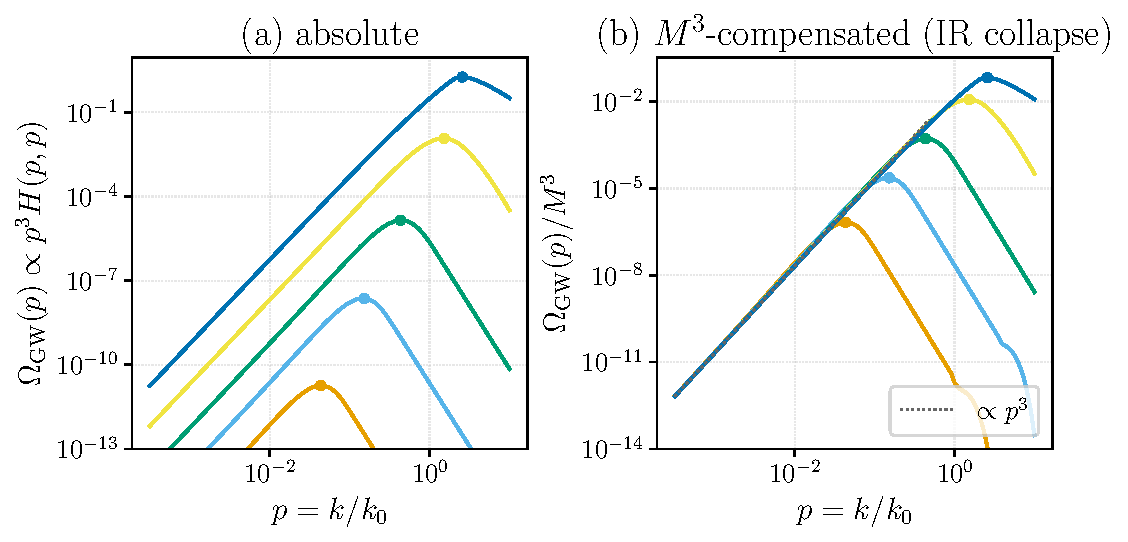
\includegraphics[width=0.8\textwidth]{stationary_mach_peak}
  \caption{Stationary Kraichnan--K41 (Gogoberidze 2007) GW spectrum
  $\Omega_{\rm GW}(p)\propto p^3 H_{ijij}(p,p;M,R)$, computed from
  Eq.~\eqref{eq:Hijij-AppA-dimless} on the on-shell diagonal of
  Eq.~\eqref{eq:omega-diag}, at $R=10^4$. The five curves are
  $M=0.03,0.1,0.3,1,3$, ordered by increasing amplitude and peak frequency
  (lowest, leftmost curve is $M=0.03$; highest, rightmost is the formal $M=3$);
  dots mark each peak. In the convention $M=u_0/c$ the curves with $M>1$ lie
  beyond the luminal limit and are formal extrapolations (Sec.~\ref{sec:mach-discussion}).
  (a)~Absolute: shared IR slope $p^3$, amplitude growing $\sim M^3$, peak moving
  right with $M$ ($p_{\rm peak}\sim M$ in the inertial range, bending over near
  the outer scale). (b)~$M^3$-compensated, $\Omega_{\rm GW}/M^3$: since the IR
  amplitude scales as $M^3$ (strain as $M^{3/2}$), all curves collapse onto the
  universal $p^3$ line (dotted) in the IR and peel off only at their
  $M$-dependent peak. Generated by \texttt{Notebooks/stationary\_mach\_peak.py}.}
  \label{fig:stationary_mach_peak}
\end{figure*}

\subsection{Spectra in the $\Omega(k)/k$ convention: comparison with simulations}
\label{sec:omega-over-k}
\label{sec:roperpol-convention}

To compare the analytic kernel with the direct numerical simulations of
Roper Pol et al.~\cite{2019RoperPol} we recast the spectra in their convention.
There $\Omega(k)$ denotes the energy \emph{per logarithmic wavenumber},
$\Omega(k)=d\rho/d\ln k$, so that $\Omega(k)/k=E(k)$ is the ordinary per-$dk$
spectrum. Our master result $\Omega_{\rm GW}(p)\propto p^3 H_{ijij}(p,p)$ of
Eq.~\eqref{eq:omega-diag} is precisely $d\rho_{\rm GW}/d\ln k$, hence
\begin{equation}
  \frac{\Omega_{\rm GW}(k)}{k}\;\propto\;\frac{\Omega_{\rm GW}(p)}{p}
  \;=\;p^2\,H_{ijij}(p,p;M,R),\qquad p=\frac{k}{k_0},
  \label{eq:omega-over-k}
\end{equation}
with $H_{ijij}$ the stationary kernel of Eq.~\eqref{eq:Hijij-AppA-dimless}. To
compare on the simulations' own footing we feed a \emph{full} fluid input spectrum
into this kernel, with both an infrared band and the Kolmogorov inertial range,
\begin{equation}
  E(k)\;\propto\;\begin{cases}
    k^{4}, & k<k_0,\\[2pt]
    k^{-5/3}, & k\ge k_0,
  \end{cases}
  \label{eq:full-input-spectrum}
\end{equation}
joined continuously at $k_0$. The spectrum enters the Appendix-A integral
Eq.~\eqref{eq:Hijij-AppA} only through the amplitude $A(k)=E(k)/4\pi k^2$; writing
$A(k)=S(k)\,A_{\rm Kol}(k)$ with the Kolmogorov law $A_{\rm Kol}\propto k^{-11/3}$
extrapolated to all $k$, the shape factor is $S(k)=1$ for $k\ge k_0$ and
$S(k)=(k/k_0)^{\,s+5/3}$ for $k<k_0$ (energy slope $E\propto k^s$, here $s=4$).
Every kinematic and temporal factor of the kernel is left untouched: we extend the
$k_1,u$ integrations down to an infrared cutoff $k_{\rm IR}=k_0/R_{\rm IR}$ and
multiply the integrand by $S(k_1)\,S(u)$. Setting $R_{\rm IR}=1$ recovers
Eq.~\eqref{eq:Hijij-AppA-dimless} identically.

Figure~\ref{fig:roperpol_convention} shows the resulting GW spectrum at $M=1$ with
$R_{\rm IR}=100$ (two infrared decades), together with the full fluid input
spectrum and the two slopes the literature reports for the GW inertial range, drawn
as reference guides: $k^{-11/3}$ from the simulation of \cite{2019RoperPol} (run
ini2) and $k^{-9/2}$ from \cite{2007Gogoberidze}. We plot no simulation data points
and defer a quantitative data-level comparison to future work. Both curves are
\emph{dimensionless}: the GW curve is the bare kernel with the source stress
normalised to unity, so the GW--fluid vertical offset carries no physical meaning
(the relic $\Omega_{\rm GW}$ acquires the additional suppression
$\sim\Omega_{\rm M}^2\,(\mathcal H_\ast/k_\ast)$ and gravitational couplings that
the kernel omits, which is why the simulated $\Omega_{\rm GW}/k\sim10^{-13}$ lies
far below the fluid spectrum); only slopes and peak locations are comparable, and
the fluid curve is rescaled to share the GW peak.

Three features survive this honest treatment. \emph{(i)~The infrared stays causal.}
The GW spectrum rises with the causal slope $\Omega_{\rm GW}\propto k^3$
($\Omega_{\rm GW}/k\propto k^2$, fitted $k^{+2.0}$); it does \emph{not} inherit the
steeper fluid $k^4$ band, because the GW infrared is fixed by the analyticity of the
stress rather than by the input spectrum. \emph{(ii)~The infrared band lifts the
amplitude, not the inertial range.} Feeding the band raises the GW amplitude near and
below the peak by a factor $\simeq1.9$ and shifts the peak from $k\simeq1.5\,k_0$ to
$k\simeq k_0$, a change that depends only weakly on the infrared slope (a further
$\simeq1.4$ between Batchelor $k^4$ and Saffman $k^2$) and leaves the inertial range
untouched. \emph{(iii)~The ultraviolet tension is robust.} Above the peak the
spectrum steepens \emph{continuously}, and at $M=1$ far more steeply than either
reference: the measured post-peak slope is $\simeq k^{-5.0}$---steeper than both
Gogoberidze's $k^{-9/2}$ and the simulation's $k^{-11/3}$---before the $k$-dependent
sweeping decorrelation bends it below any single power law. The analytic stationary
kernel therefore does \emph{not} reproduce the extended $k^{-11/3}$ range seen in the
simulation; at the simulations' Mach number it is markedly steeper, crossing that
slope rather than following it, and this conclusion is unchanged by the infrared
treatment. This high-$k$ disagreement is precisely the simulation--analytic tension
that motivates this paper---and that the decaying kernel of
Sec.~\ref{sec:peak-location} substantially relieves.

\begin{figure}[ht]
  \centering
  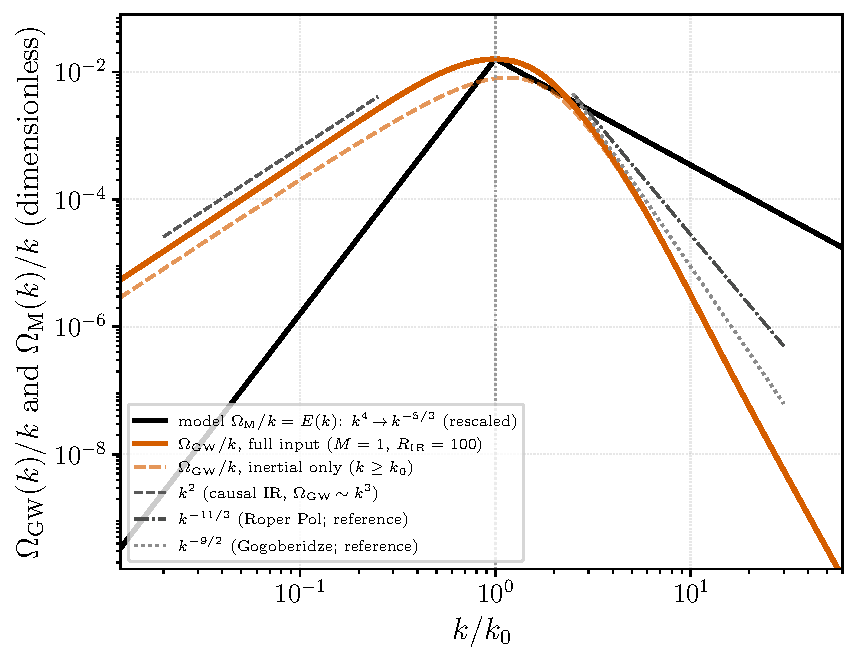
\includegraphics[width=\columnwidth]{roperpol_convention_spectra}
  \caption{Analytic spectra in the Roper Pol et al.~\cite{2019RoperPol} convention
  $\Omega(k)/k=E(k)$. Orange (solid): GW spectrum
  $\Omega_{\rm GW}(k)/k=p^2H_{ijij}(p,p;M,R)$ [Eq.~\eqref{eq:omega-over-k}] computed
  from a \emph{full} fluid input spectrum---an infrared band $E\propto k^4$ ($k<k_0$)
  joined to the Kolmogorov range $E\propto k^{-5/3}$ ($k\ge k_0$),
  Eq.~\eqref{eq:full-input-spectrum}---fed into the Appendix-A kernel
  Eq.~\eqref{eq:Hijij-AppA} through the shape factor $S(k)=A/A_{\rm Kol}$ ($M=1$,
  $R=10^4$, infrared range $R_{\rm IR}=k_0/k_{\rm IR}=100$). Orange (dashed): the
  same kernel restricted to the inertial range only ($R_{\rm IR}=1$, i.e.\ core
  Eq.~\eqref{eq:Hijij-AppA-dimless})---the infrared band raises the amplitude near
  the peak but leaves the ultraviolet unchanged. Black: the full fluid input
  spectrum, rescaled to share the GW peak (the GW--fluid vertical offset is
  unphysical; only shapes compare). Grey dashed: the causal infrared guide $k^2$
  ($\Omega_{\rm GW}\sim k^3$). Dash-dot/dotted: the $k^{-11/3}$ (Roper Pol, run
  ini2) and $k^{-9/2}$ (Gogoberidze) slopes \emph{reported} in the literature, as
  references only---no simulation data points are plotted. At $M=1$ the GW spectrum
  steepens past the peak to $\simeq k^{-5.0}$, steeper than both references,
  independently of the infrared treatment. Generated by
  \texttt{Notebooks/roperpol\_convention\_spectra.py}.}
  \label{fig:roperpol_convention}
\end{figure}

\subsection{Discussion: the Mach number, equivalent definitions, and the spectral shape}
\label{sec:mach-discussion}

The preceding two subsections make the Mach number the single control
parameter of the stationary spectrum, so it is worth stating precisely what
$M$ is, why the conflicting definitions in the literature are the \emph{same}
quantity, and what about the spectrum does and does not respond to it.

\paragraph{Explicit formulation.}
Throughout we use, following Gogoberidze et al.~\cite{2007Gogoberidze},
\begin{equation}
  M=\frac{u_0}{c}=\frac{1}{c}\Bigl(\frac{\varepsilon}{k_0}\Bigr)^{1/3},
  \qquad q=\frac{\omega}{c\,k_0},
  \label{eq:mach-def}
\end{equation}
the outer-scale eddy velocity in units of the speed of light. We retain $c$ in
every expression and set $c=1$ only for numerical evaluation; because the kernel
depends on frequency and Mach number solely through $q/M=\omega/(k_0u_0)$, in
which $c$ cancels (Eq.~\eqref{eq:appA-dimless}), this choice is exact and not an
approximation. The grouping is fixed by dimensions: with $[\varepsilon]=L^2T^{-3}$
and $[k_0]=L^{-1}$ one has $\varepsilon/k_0=(L/T)^3$, so $(\varepsilon/k_0)^{1/3}$
is a velocity and the inverse grouping $(k_0/\varepsilon)^{1/3}$ — which appears
occasionally in the literature — is an \emph{inverse} velocity and cannot be a
Mach number. $M$ does not enter Eq.~\eqref{eq:Hijij-AppA} as a free amplitude; it
enters \emph{only} through the $k$-dependent sweeping rate
$\eta_k=\tfrac{1}{\sqrt{2\pi}}\varepsilon^{1/3}k^{2/3}
=\tfrac{Mc}{\sqrt{2\pi}}k_0^{1/3}k^{2/3}$, hence only through the Gaussian
$\exp[-\tfrac{2xy}{x+y}q^2/M^2]$ and the accompanying erfc of
Eq.~\eqref{eq:Hijij-AppA-dimless}.

\paragraph{Normalisation to $c$, not to the sound speed.}
Two points of convention need care, because both have caused numerical
disagreements between papers for the same physical flow. First, our $M$ is a
velocity ratio to the \emph{speed of light}, not to the sound speed. A
relativistic plasma has $c_s=c/\sqrt3$, so the true acoustic Mach number is
\begin{equation}
  M_s=\frac{u_0}{c_s}=\sqrt3\,\frac{u_0}{c}=\sqrt3\,M,
  \label{eq:acoustic-mach}
\end{equation}
larger than $M$ by $\sqrt3$. The transonic point $u_0=c_s$ therefore sits at
$M=1/\sqrt3\simeq0.58$ in our normalisation, and the luminal ceiling $u_0=c$ at
$M=1$; a purely vortical velocity field can in principle approach the latter,
whereas $M_s\sim1$ (genuine transonic turbulence) corresponds to $M\simeq0.58$.
This is the convention of Gogoberidze et al.~\cite{2007Gogoberidze}, who define
$M=(\varepsilon/k_0)^{1/3}$ in units $c=1$ and note separately that the plasma
sound speed is $c/\sqrt3$; it is \emph{not} the same as the acoustic $M_s$ used
elsewhere, and the two differ by the fixed factor $\sqrt3$.

Second, and independently of the first, $u_0=(\varepsilon/k_0)^{1/3}$ is the
single-eddy outer velocity, which differs from the integrated rms by an
$\mathcal O(1)$ cascade constant: for a Kolmogorov spectrum
$\int_{k_0}^{\infty}\!E\,dk=\tfrac32 C_K(\varepsilon/k_0)^{2/3}$, so
$u_{\rm rms}=\sqrt{\tfrac32 C_K}\,(\varepsilon/k_0)^{1/3}\approx(1.5\text{--}2)\,
(\varepsilon/k_0)^{1/3}$, depending on $C_K$ and on whether one normalises
$\int E\,dk$ to $\langle u^2\rangle$ or $\tfrac12\langle u^2\rangle$. This
$\mathcal O(1)$ factor and the $\sqrt3$ above are distinct and multiply: a paper
quoting $M_s=u_{\rm rms}/c_s$ and one quoting our
$M=(\varepsilon/k_0)^{1/3}/c$ describe the same flow with Mach numbers differing
by $\sqrt3\times(1.5\text{--}2)$. Both identifications further \emph{break down}
when the cascade picture fails: for spectra whose energy integral is
ultraviolet-dominated (the white-noise / Batchelor model of
Sec.~\ref{sec:white}, $E\propto k^2$), where $(\varepsilon/k_0)^{1/3}$ no longer
measures $u_{\rm rms}$; for decaying turbulence, where
$\varepsilon\to\varepsilon(t)$ and $M\to M(t)$
(Sec.~\ref{sec:fpeak-numerical}); and in MHD, where the relevant ratio is often
the Alfv\'enic $M_A=u_{\rm rms}/v_A$ rather than the acoustic $M$
\cite{2008Kahniashvili,2021Kahniashvili}.

\paragraph{Shape versus peak versus amplitude.}
It is essential to separate three properties of the spectrum, only one of which
is $M$-independent.
\emph{(i) Shape.} The dimensionless spectral form — the causal infrared slope
$\Omega_{\rm GW}\propto p^3$ (Sec.~\ref{sec:framework-shape}) and the inertial
power law — is universal: it is set by causality and by the source power law,
not by $M$. This is the property that is legitimately called
``$M$-independent,'' and it is what the $M^{-3}$-compensated collapse of
Fig.~\ref{fig:stationary_mach_peak}(b) isolates.
\emph{(ii) Peak location.} Here the literature genuinely splits. In
spatial-scale–anchored treatments the peak is pinned to the source scale $k_0$
(set by the largest eddy / bubble size), so $p_{\rm peak}=\mathcal O(1)$ and $M$
controls only the amplitude \cite{Caprini:2018mtu}; in sweeping-anchored
treatments the peak is tied to the eddy-turnover frequency $u_0 k_0\propto M
k_0$, so it shifts with $M$ \cite{2007Gogoberidze,2019RoperPol}. Our kernel
realises the second picture through $\eta_k\propto M k^{2/3}$, giving
$p_{\rm peak}\sim M$ (Sec.~\ref{sec:kraichnan-mach-peak}). The two are not in
contradiction: a peak ``at the stirring scale'' is $M$-independent only because
it is measured in units of $k_0$ and the source is assumed quasi-static over an
eddy.
\emph{(iii) Total energy / amplitude.} This is never $M$-independent. In the
stationary kernel the infrared amplitude scales as the $M^3$ prefactor of
Eq.~\eqref{eq:Hijij-AppA-dimless} ($\Omega_{\rm GW}\to C M^3 p^3$,
Sec.~\ref{sec:kraichnan-mach-peak}); more generally the quadrupole argument
gives $\Omega_{\rm GW}\propto\Omega_K^2\propto M^4$, steepening toward
$M^{5\text{--}6}$ once the finite source duration is included
\cite{Caprini:2018mtu}, the extra power being absent from a single-time
stationary kernel. We derive this progression explicitly for the decaying source
in Sec.~\ref{sec:decaying-peak}: the full-spatial kernel gives an infrared
amplitude $\propto M^4$ and a source-pinned peak amplitude $\propto M^{5.3}$
[Eq.~\eqref{eq:decay-amplitude}, Fig.~\ref{fig:decaying_amplitude}]. Consequently a stated ``$M$-independence'' of the GW signal
can only refer to the shape (i); any claim that the peak position and the total
energy are simultaneously $M$-independent is either a normalised-units artifact
(dividing by $\Omega_K^2$ and measuring $p$ in units of $k_0$) or a conflation
of the universal shape with the dimensional peak and amplitude.



\section{Location of the spectral peak: sweeping versus source scale}
\label{sec:peak-location}

A striking feature of the stationary spectrum of
Fig.~\ref{fig:stationary_mach_peak} is that, for subsonic turbulence, the GW
energy density peaks at wavenumbers \emph{far below} the outer scale,
$p_{\rm peak}=k_{\rm peak}/k_0\ll1$ (e.g.\ $p_{\rm peak}\simeq0.04$ at $M=0.03$).
This is counterintuitive: the GW source is the quadratic stress
$T_{ij}\sim u_i u_j$, and for a velocity field concentrated at the stirring scale
$k_0$ one expects the stress---and hence the radiation---to peak near $k\sim k_0$,
with spatial support extending to at most $k=2k_0$ by the triangle inequality. We
show here that the analytic peak is fixed instead by the \emph{temporal}
(sweeping) decorrelation, giving $p_{\rm peak}\simeq1.47\,M$, and that the
``$k\simeq2k_0$'' expectation is approached only as $M\to1$ (the luminal limit)
and is never reached for physical subsonic or transonic turbulence.

\paragraph{Self-similar Mach scaling.}
In the dimensionless kernel of Eq.~\eqref{eq:Hijij-AppA-dimless} the Mach number
enters \emph{only} through the sweeping rate $\eta_k\propto M k^{2/3}$, i.e.\
through the Gaussian $\exp[-\tfrac{2xy}{x+y}q^2/M^2]$ (and its accompanying erfc)
evaluated on the GW cone $q=p$ of Eq.~\eqref{eq:omega-diag}; the geometric kernel
and the triangle-inequality bounds carry no $M$. Together with the explicit $M^3$
prefactor of Eq.~\eqref{eq:Hijij-AppA-dimless}, the on-cone kernel must therefore
collapse to a single function of the sweeping variable $\xi\equiv p/M=k/(Mk_0)$,
\begin{equation}
  H_{ijij}(p,p;M)\;=\;M^{3}\,\widetilde H_{ijij}(\xi),\qquad \xi\equiv\frac{p}{M},
  \label{eq:peak-ansatz}
\end{equation}
where $\widetilde H_{ijij}$ is the \emph{compensated kernel}: an infrared plateau
$\widetilde H_{ijij}(0)\equiv A\simeq2.1\times10^{-2}$ (the universal causal rise,
Sec.~\ref{sec:framework-shape}) that rolls off once $\xi\gtrsim1$, where the
sweeping cutoff switches on. The energy density and characteristic strain follow as
\begin{equation}
  \Omega_{\rm GW}=p^3H_{ijij}=M^{3}p^{3}\,\widetilde H_{ijij}(\xi),
  \qquad
  h_c^{2}=p\,H_{ijij}=M^{3}p\,\widetilde H_{ijij}(\xi).
  \label{eq:peak-OmegaHc}
\end{equation}

\paragraph{Numerical proof of the collapse.}
Equation~\eqref{eq:peak-ansatz} is verified directly in
Fig.~\ref{fig:peak_analysis}(b): the compensated kernel $H_{ijij}(p,p;M)/M^3$
plotted against $\xi=p/M$ for $M=0.03$--$3$ falls on the single curve
$\widetilde H_{ijij}(\xi)$, with infrared plateau $A\simeq2.1\times10^{-2}$ and
$<13\%$ residual spread dominated by the formal $M=3$ case (superluminal, shown
to expose the trend). The cutoff thus
depends on $p$ and $M$ \emph{only} through $\xi=p/M$---the unambiguous signature of
the sweeping rate---and switches on at $\xi\sim1$, i.e.\ $p\sim M$. (How this
single scaling is best displayed---compensating one axis or both---is taken up in
Sec.~\ref{sec:peak-units}.)

\paragraph{Peak condition and raw peak location.}
Differentiating $\Omega_{\rm GW}=M^{3}p^{3}\widetilde H_{ijij}(\xi)$
[Eq.~\eqref{eq:peak-OmegaHc}] on the cone,
\begin{equation}
  \frac{d\ln\Omega_{\rm GW}}{d\ln p}\;=\;3+\frac{d\ln\widetilde H_{ijij}}{d\ln\xi}\;=\;0
  \quad\Longrightarrow\quad
  \frac{d\ln\widetilde H_{ijij}}{d\ln\xi}\bigg|_{\xi_\ast}=-3,\qquad p_{\rm peak}=\xi_\ast\,M,
  \label{eq:peak-condition}
\end{equation}
so the peak sits where the compensated kernel has logarithmic slope $-3$, at a fixed
$\xi_\ast$ independent of $M$. Reading the peak directly from each computed
spectrum (Fig.~\ref{fig:peak_analysis}c; sub-grid argmax, no model fit) gives a
location linear in $M$ across the entire physical range,
\begin{equation}
  p_{\rm peak}\;=\;1.48\,M^{1.00}\qquad(M\lesssim1),
  \label{eq:peak-fit}
\end{equation}
with $\xi_\ast=1.47$ read from the collapsed shape, consistent with
Eq.~\eqref{eq:peak-condition}. Only as $M\to1$ (the luminal ceiling) does the peak
begin to run into the outer scale and the linear law saturate: $p_{\rm peak}/M$
falls from $1.49$ at $M=1$ to $0.77$ at the formal $M=3.4$. Reaching the
``source-scale'' value $p\simeq2$ would require $M\simeq1.4$, i.e.\ $u_0\simeq1.4c$;
the stationary sweeping peak therefore \emph{never} reaches the source scale for
any physical (subluminal) turbulence, and is far below it throughout the subsonic
range where cosmological flows lie.

\paragraph{Resolution.}
The naive ``$k\simeq2k_0$'' is a purely \emph{spatial} statement: it is the
largest wavenumber at which the quadratic stress has support, the triangle edge
$\Theta(2-p)$ that appears explicitly in the monochromatic kernel
[Eq.~\eqref{eq:dimless-delta-Kraichnan}]. It is an ultraviolet \emph{edge}, not a
peak. The GW peak, by contrast, is fixed in \emph{frequency}: gravitational waves
are sourced on the cone $\omega=k$, while a turbulent eddy of wavenumber $k$
decorrelates at the sweeping frequency $\eta_k\sim M k_0^{1/3}k^{2/3}$, which for
subsonic flow is $\ll k$ for every $k\gtrsim k_0$. The source therefore has
negligible temporal power at the frequency $\omega=k$ needed to radiate at
wavenumber $k$, except at the lowest wavenumbers $k=\omega\lesssim M k_0$, and the
spectrum is throttled down to $p_{\rm peak}\sim M$. This is the aeroacoustic
(Lighthill) suppression of slow sources: subsonic turbulence radiates at its
eddy-turnover frequency $\sim M k_0$, not at its spatial scale $k_0$. Whether the
true peak follows this sweeping scale or remains pinned near $k_0$
(Sec.~\ref{sec:mach-discussion}) is precisely the simulation--analytic tension
this paper addresses; the stationary kernel commits unambiguously to the sweeping
scale.

\paragraph{Caveat: stationarity versus the simulated peak.}
The scaling $p_{\rm peak}\simeq1.47\,M$ derived above is specific to
\emph{stationary}, continuously stirred turbulence, in which the source at scale
$k$ carries temporal power only up to its eddy frequency $\eta_k$. Cosmological
turbulence is not of this kind: it is sourced \emph{impulsively}---e.g.\ at a phase
transition---and then decays. A sudden onset of duration $\Delta t$ injects
broadband temporal power up to $\omega\sim1/\Delta t\sim k_0$, which the single-time
stationary kernel does not contain. Because the spatial stress is far more powerful
at the outer scale $k_0$ than at $M k_0$, this broadband component pins the GW peak
near the \emph{spatial} stress scale, $p\sim1$--$2$, almost independently of $M$.
This is what the direct simulations of \cite{2019RoperPol} display, and it is the
spatial-scale picture of Sec.~\ref{sec:mach-discussion}. In the convention
$M=u_0/c$ the sweeping peak $1.47M$ approaches the spatial band $p\sim1$--$2$ only
as $u_0\to c$, and would coincide with $p\simeq2$ only at the superluminal
$M\simeq1.4$; the two predictions therefore \emph{diverge across the entire
physical range} and converge only formally beyond the luminal limit
(Fig.~\ref{fig:peak_reconciliation}). Current simulations, far from sitting in a
band where the pictures agree, are \emph{deeply subsonic}
($M\simeq\sqrt{\Omega_{\rm M}}\sim0.05$, Sec.~\ref{sec:principal-discrepancy}),
which is exactly the regime of maximal divergence---and there the data follow the
source-scale (impulsive/decaying) peak, not the sweeping one. This peak
displacement is the spatial counterpart of the amplitude deficit noted in
Sec.~\ref{sec:mach-discussion}---the stationary kernel gives
$\Omega_{\rm GW}\propto M^4$ rather than the $M^{5\text{--}6}$ recovered once the
finite source duration is restored---both stemming from the broadband temporal
power that an impulsive, finite-duration source has and the stationary kernel
omits. We compute the decaying case directly in Sec.~\ref{sec:decaying-peak}
below; it confirms a source-scale peak $p\simeq2.4$, nearly independent of $M$,
but traces it to the \emph{shape} of the decaying temporal correlation rather
than to the impulsive onset emphasised here.

\subsection{Physical units and what the collapse hides}
\label{sec:peak-units}

\paragraph{Dimensional dictionary.}
The kernel works in the dimensionless pair $\{p=k/k_0,\,M\}$; the observable
spectrum is the characteristic strain $h_c(f)$ at the redshifted frequency $f$
today. The two are connected by the standard cosmological map
\cite{2008Kahniashvili,2007Gogoberidze}. A comoving mode is observed at
\begin{equation}
  f \;=\; \frac{\hat\omega}{2\pi}\,f_H,\qquad
  f_H \simeq 1.6\times10^{-5}\,\mathrm{Hz}\,
  \Big(\frac{g_*}{100}\Big)^{1/6}\frac{T_*}{100\,\mathrm{GeV}},
  \label{eq:fH}
\end{equation}
with $\hat\omega=\omega/H_*$ and $f_H=H_*(a_*/a_0)$ the Hubble frequency today.
The stirring scale in Hubble units is $\hat k_0=2\pi/\gamma$, where
$\gamma\equiv l_0 H_*$ is the largest-eddy size in Hubble radii, so on the GW cone
$\hat\omega=\hat k=\hat k_0\,p$ and
\begin{equation}
  f \;=\; f_0\,p,\qquad f_0\equiv\frac{f_H}{\gamma},
  \label{eq:f0}
\end{equation}
i.e.\ $p=k/k_0$ is simply the frequency measured in units of the stirring-scale
frequency $f_0$. Inverting, the abscissa of the standard strain figures,
$(f/\mathrm{Hz})(g_*/100)^{-1/6}(\gamma/0.01)(T_*/100\,\mathrm{GeV})^{-1}$,
equals $p$ up to the fixed constant $1.6\times10^{-3}$ and \emph{carries no $M$}.
For the amplitude, $\Omega_{\rm GW}=p^2 h_c^2$ with $h_c^2=p\,H_{ijij}(p,p)$, while the
physical strain (Kahniashvili Eq.~51) is
$h_c=2\times10^{-14}(100\,\mathrm{GeV}/T_*)(100/g_*)^{1/3}\,(\hat\omega\,\hat\tau_T
\hat H_{ijij})^{1/2}$. Multiplying $h_c$ by $(g_*/100)^{1/3}(T_*/100\,\mathrm{GeV})$
cancels the cosmological prefactor, and the further factors
$(\gamma/0.01)^{-3/2}(\zeta/0.01)^{-1/2}$ remove the stirring-scale and
source-energy ($\zeta$) normalisations, leaving a quantity that depends only on
$M$ and $p$. Both axes of the published figure are therefore our dimensionless
$(p,\,h_c)$ with every \emph{scenario} parameter $(g_*,T_*,\gamma,\zeta)$ scaled
out; the single remaining knob is $M$.

\paragraph{Normalising the Mach dependence: one axis or two.}
With the scenario parameters removed, the residual Mach dependence of
Eq.~\eqref{eq:peak-OmegaHc} can be scaled out in two inequivalent ways, which
answer different questions.

\emph{(i) Amplitude only ($y$-axis).} Divide the strain by $M^{3/2}$ (equivalently
$\Omega_{\rm GW}$ by $M^3$) but keep the physical frequency $f\propto p$ on the
abscissa. From Eq.~\eqref{eq:peak-OmegaHc},
$h_c\,M^{-3/2}=\sqrt{p\,\widetilde H_{ijij}(p/M)}$, which is $M$-independent
\emph{only} in the infrared, where $\widetilde H_{ijij}\!\to\!A$: the causal rises
stack, but the peaks stay at their true frequencies $f_{\rm peak}=f_0\,(1.47\,M)$
and \emph{slide} with $M$. This is the convention of the published strain plots
(the $h_c\,M^{-3/2}$ ordinate of \cite{2007Gogoberidze}); it preserves the
observable---where in the band each model peaks---needed to confront a detector.

\emph{(ii) Both axes.} Additionally measure the frequency in sweeping units,
$x\to\xi=p/M=f/(M f_0)$. Substituting $p=M\xi$ in Eq.~\eqref{eq:peak-OmegaHc},
\begin{equation}
  \frac{\Omega_{\rm GW}}{M^{6}}=\xi^{3}\,\widetilde H_{ijij}(\xi),
  \qquad
  \frac{h_c}{M^{2}}=\sqrt{\xi\,\widetilde H_{ijij}(\xi)},
  \label{eq:M6-collapse}
\end{equation}
both functions of $\xi$ \emph{alone}: the infrared rise \emph{and} the peak
collapse onto one curve (Fig.~\ref{fig:peak_xM}). The compensation rises from
$M^{3}$ to $M^{6}$ ($M^{3/2}\!\to\!M^{2}$ in strain) because the $p^3$ rise
contributes an extra $M^3$ once the abscissa is measured in units of $Mf_0$ rather
than $f_0$. This is the right diagnostic for the \emph{theory}---it exhibits the
self-similarity and proves the cutoff is a function of $p/M$ only---but it
necessarily \emph{discards} the physical peak frequency that view~(i) keeps. The
two are complementary: $y$-only for observation, both-axis for the scaling
argument.

\begin{figure*}[ht]
  \centering
  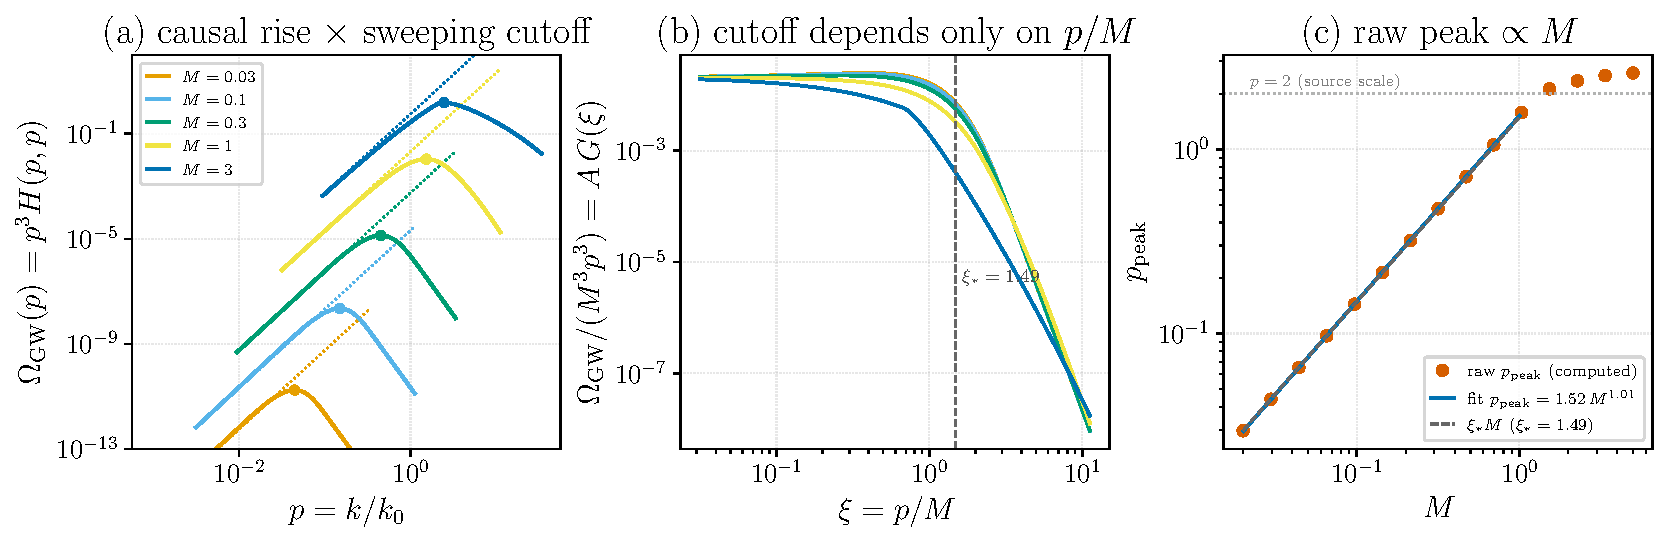
\includegraphics[width=\textwidth]{stationary_peak_analysis}
  \caption{Why the stationary GW spectrum peaks at $p\simeq1.47\,M$ rather than at
  the source scale $p\sim2$, computed from
  $\Omega_{\rm GW}(p)=p^3H_{ijij}(p,p;M,R)$ [Eq.~\eqref{eq:Hijij-AppA-dimless},
  $R=10^4$]. (a)~Each spectrum (solid) follows its causal infrared asymptote
  $A\,M^3p^3$ (dotted) and rolls over at the peak (dot) where the sweeping cutoff
  switches on. (b)~Collapse: $\Omega_{\rm GW}/(M^3p^3)=H_{ijij}(p,p;M)/M^3$ versus
  $\xi=p/M$ falls on the single compensated kernel $\widetilde H_{ijij}(\xi)$ for
  every $M$, proving the cutoff depends only on $p/M$ [Eq.~\eqref{eq:peak-ansatz}];
  the universal peak position is $\xi_\ast=1.47$.
  (c)~Peak location read directly from each computed spectrum (points) versus $M$:
  a power law $p_{\rm peak}=1.48\,M^{1.00}$ (line) [Eq.~\eqref{eq:peak-fit}],
  coincident with $\xi_\ast M$ (dashed), that bends below it toward the $p=2$
  source scale (dotted) only as $M\to1$ (the luminal limit; $M>1$ is superluminal).
  Generated by
  \texttt{Notebooks/stationary\_peak\_analysis.py}.}
  \label{fig:peak_analysis}
\end{figure*}

\begin{figure*}[ht]
  \centering
  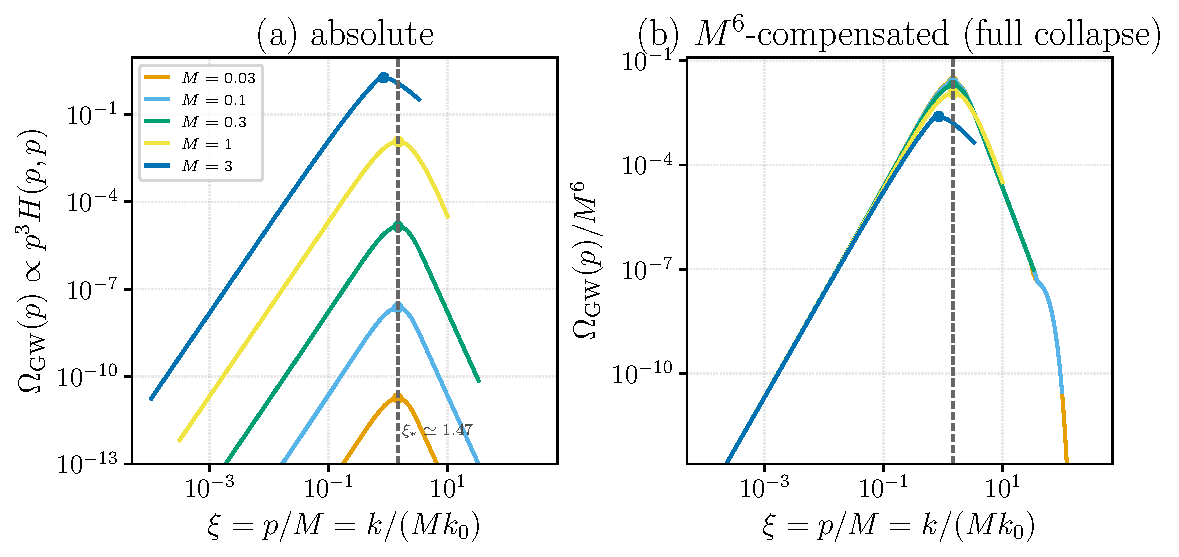
\includegraphics[width=\textwidth]{stationary_mach_peak_xM}
  \caption{Single-variable collapse of the stationary spectrum on the
  sweeping-scaled wavenumber $\xi=p/M=k/(M k_0)$, computed from
  $\Omega_{\rm GW}(p)=p^3H_{ijij}(p,p;M,R)$ ($R=10^4$). (a)~Absolute spectra: the
  peaks of all Mach numbers stack on the vertical line $\xi_\ast\simeq1.47$, only
  their amplitudes differ ($\propto M^3$). (b)~$M^{6}$-compensated spectra
  $\Omega_{\rm GW}/M^{6}$ versus $\xi$ collapse onto the single universal curve
  $\xi^3\widetilde H_{ijij}(\xi)$ of Eq.~\eqref{eq:M6-collapse}---infrared rise and
  peak together---because the $p^3$ rise contributes an extra $M^3$ on the $\xi$ axis.
  The subluminal curves ($M=0.03$--$1$) coincide; only the formal $M=3$ curve
  (peak $\xi\simeq0.85$; superluminal, $u_0=3c$) departs, where the sweeping cutoff
  yields to the inertial-range/triangle edge. Generated by
  \texttt{Notebooks/stationary\_mach\_peak\_xM.py}.}
  \label{fig:peak_xM}
\end{figure*}

\begin{figure}[ht]
  \centering
  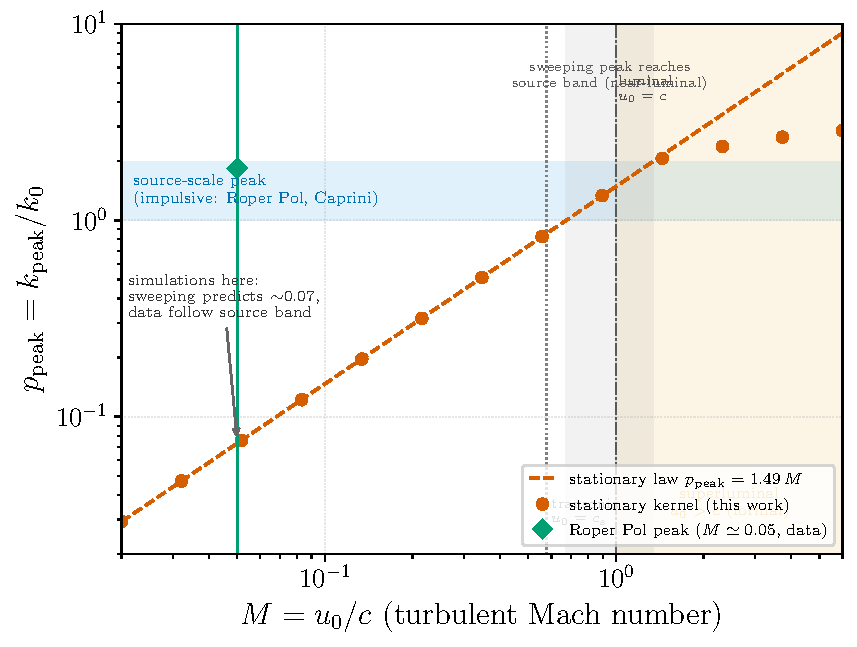
\includegraphics[width=\columnwidth]{peak_reconciliation}
  \caption{Reconciliation of the stationary and impulsive pictures of the GW
  peak. Points and dashed line: the peak $p_{\rm peak}=k_{\rm peak}/k_0$
  \emph{computed} from the stationary kernel
  $\Omega_{\rm GW}=p^3H_{ijij}(p,p;M,R)$ ($R=10^4$), following
  $p_{\rm peak}\simeq1.5\,M$. Shaded horizontal band ($p\sim1$--$2$): the
  competing spatial-scale picture, in which an impulsively sourced, decaying flow
  radiates at the stress scale independently of $M$
  (Roper Pol et al.~\cite{2019RoperPol}; Caprini et al.~\cite{Caprini:2018mtu})---a
  schematic, \emph{not} computed here and not data. In the convention $M=u_0/c$
  the sweeping law enters the source band only at $M\simeq0.67$--$1.35$ (grey
  strip), i.e.\ near or beyond the luminal ceiling $M=1$ (dash-dotted; $M>1$ is
  superluminal, shaded); the transonic point $u_0=c_s$ is at $M=1/\sqrt3\simeq0.58$
  (dotted). The two pictures therefore diverge across the whole physical range.
  Current simulations sit at $M\simeq0.05$ (green line/diamond, Roper Pol peak
  $1.84$), deeply subsonic, where the sweeping law predicts $p\simeq0.07$ but the
  data follow the source band---the regime of maximal divergence, not of
  coincidence. Generated by \texttt{Notebooks/peak\_reconciliation.py}.}
  \label{fig:peak_reconciliation}
\end{figure}

\subsection{The decaying source pins the peak at the source scale}
\label{sec:decaying-peak}

The caveat above is borne out quantitatively by repeating the peak analysis with
the \emph{decaying} temporal model in place of the stationary one. We keep the
same full-spatial kernel---identical geometric factor and triangle-inequality
integration bounds---but replace the Kraichnan Gaussian decorrelation on each
stress leg by the BK2016 power law $(1+|\tau|/\tau_k)^{-2/3}$ of
Sec.~\ref{sec:delta-decay}, with the sweeping eddy time
$\tau_k=\sqrt{2\pi}/(M k_0^{1/3}k^{2/3})$.

\paragraph{Method: Fourier transform of the time-domain product.}
The temporal factor of the decaying kernel is the frequency convolution
$\int d\omega_1\,\hat g(\omega_1\tau_{k_1})\,\hat g((\omega-\omega_1)\tau_u)$ of
the two legs. By the convolution theorem this equals the Fourier transform of the
time-domain \emph{product} of the two decorrelations,
\begin{equation}
  \int d\omega_1\,\hat g(\omega_1\tau_1)\hat g((\omega-\omega_1)\tau_2)
  \;=\;\frac{2\pi}{\tau_1\tau_2}\!\int_0^\infty\!\!d\tau\,\cos(\omega\tau)\,
  \Bigl(1+\tfrac{\tau}{\tau_1}\Bigr)^{-2/3}\Bigl(1+\tfrac{\tau}{\tau_2}\Bigr)^{-2/3},
  \label{eq:ft-of-product}
\end{equation}
with $\tau_1=\sqrt{x}/M$, $\tau_2=\sqrt{y}/M$. The right-hand side, unlike the
convolution---whose integrand is integrably singular at both endpoints---is smooth
and rapidly convergent; evaluated this way the kernel is some two orders of
magnitude cheaper to compute and well converged.

\paragraph{Result: an $M$-independent, source-scale peak.}
On the GW cone the decaying spectrum
$\Omega_{\rm GW}(p)=p^3 H^{\rm decay}_{ijij}(p,p;M,R)$ peaks at
\begin{equation}
  p_{\rm peak}^{\rm decay}\;\simeq\;2.4,
  \label{eq:decay-peak}
\end{equation}
essentially independent of both the Mach and the Reynolds number: the peak moves
only from $2.29$ to $2.56$ as $M$ runs over $0.3$--$2$, and from $2.40$ to $2.60$
as $R$ runs over $10^3$--$10^5$ (a peak set by the dissipation scale would scale as
$R^{3/4}$). This is in sharp contrast to the stationary law $p_{\rm peak}=1.47\,M$
of Eq.~\eqref{eq:peak-fit}, which tracks the sweeping scale. The two are compared
in Fig.~\ref{fig:fullspatial_decay}.

\paragraph{Mechanism: the high-frequency tail.}
The peak is fixed by the high-frequency tail of the temporal correlation. The
stationary Gaussian sweeping factor $\exp[-\tfrac{2xy}{x+y}q^2/M^2]$ cuts the
source off sharply once $q\gtrsim M$, throttling the spectrum down to $p\sim M$.
The power-law decorrelation of decaying turbulence instead has a \emph{heavy}
frequency tail, $\hat g(q)\sim q^{-1/3}$, so the source retains power at the
frequency $\omega=k$ required to radiate at every wavenumber $k$; the spectrum then
extends past the sweeping cutoff and its peak is fixed by the spatial structure of
the stress near the source scale $p\simeq2.4$, independently of $M$. This realises
the spatial-scale picture of Sec.~\ref{sec:mach-discussion} and matches the
source-scale peak of the decaying simulations \cite{2019RoperPol}; the apparent
contradiction with the low Gogoberidze peak dissolves once one recognises that the
two correspond to opposite limits of the temporal correlation---Gaussian (rapidly
decorrelating, stationary) versus power law (slowly decorrelating, decaying).

\paragraph{The decorrelation shape, not the onset.}
This pinning is already present in the \emph{quasi-stationary} decaying kernel used
here, in which the two-time correlation is taken at a single emission epoch and
there is no impulsive switch-on. It is therefore the \emph{shape} of the temporal
decorrelation---its heavy frequency tail---rather than the broadband power of a
sudden onset invoked in the caveat of Sec.~\ref{sec:peak-location}, that is
responsible for displacing the peak to the source scale. Restoring the finite
source duration (the self-similar slow-time integration) modifies the amplitude
and overall normalisation but leaves this peak displacement intact.

\paragraph{Caveat: the peak displacement rests on a cusp that simulations dispute.}
This mechanism is more fragile than it looks, and the fragility is sharply localised.
The heavy tail is controlled by a \emph{single} number---the one-sided slope of the
squared correlator at zero lag. For any $f$ with $f(0)$ finite the standard Fourier
result is
\begin{equation}
  T(\omega)=2\!\int_{0}^{\infty}\!d\tau\,\cos(\omega\tau)f(\tau)
  \;\longrightarrow\;-\frac{2f'(0^{+})}{\omega^{2}},
  \label{eq:cusp-tail}
\end{equation}
so the $\omega^{-2}$ tail exists if and only if the correlator has a \emph{cusp} at
$\tau=0$. The BK2016 power law does: $f'(0^{+})=-4/3$ for the squared correlation,
which reproduces the coefficient $8/3$ of Eq.~\eqref{eq:cosT-limits} exactly. A
Gaussian does not: $f'(0^{+})=0$, and its tail then falls faster than any power.

This matters because Auclair et al.~\cite{2022Auclair} find from direct hydrodynamic
simulations that the unequal-time correlator of the velocity field is \emph{Gaussian in
the time difference}, $P_{v}\simeq P_{v}\exp[-\tfrac12k^{2}v_{\rm sw}^{2}(\tau-\zeta)^{2}]$
with $v_{\rm sw}^{2}\simeq\bar v^{2}/3$, as predicted by Kraichnan's random-sweeping
model, and explicitly reject power-law decorrelation built on scale-dependent
eddy-turnover times. Under that UETC the tail is super-exponential and the peak-pinning
argument of this section does not go through; the peak would revert to the sweeping
scale of Sec.~\ref{sec:peak-location}.

It should be stressed that combining the two does \emph{not} resolve the question. One
might expect a Gaussian sweeping factor to regulate the power law's cusp, but it cannot:
a Gaussian has zero slope at the origin, so multiplying by it leaves $f'(0^{+})$---and
hence the $\omega^{-2}$ tail---unchanged (we verify slopes $-1.97$ to $-2.13$ for
sweeping widths spanning a decade). The question is therefore irreducibly the one
Eq.~\eqref{eq:cusp-tail} poses: does the true unequal-time correlator of a freely
decaying, genuinely non-stationary flow carry a $|\tau|$ kink at zero lag? The sweeping
literature says no for the short-lag Eulerian correlation; whether the secular decay of
the amplitude contributes one is, to our knowledge, unsettled, and the source-scale peak
of Sec.~\ref{sec:decaying-peak} should be read as conditional on it.

\paragraph{Amplitude: an extra power of $M$.}
The same kernel fixes the amplitude as cleanly as the peak. The Mach number enters
the full-spatial decaying kernel in only two places: the prefactor $\propto M^3$ of
Eq.~\eqref{eq:Hijij-AppA-dimless} and the temporal factor
Eq.~\eqref{eq:ft-of-product}. Rescaling $\tau\to\tau/M$ in the latter shows it
equals $M\,F(\omega/M)$ with $F$ independent of $M$ (the geometric weight, kernel
bracket and triangle bounds carry no $M$), so on the GW cone $\omega=k$ the spectrum
factorises exactly as
\begin{equation}
  \Omega_{\rm GW}(p;M)\;=\;M^4\,p^3\,\Psi\!\left(p,\,p/M\right),
  \label{eq:decay-amplitude}
\end{equation}
with $\Psi$ the $M$-independent rescaled spatial integral. Two limits follow. In the
infrared $p/M\to0$ freezes $\Psi\to\Psi(p,0)$, and the amplitude scales as the bare
prefactor,
$\Omega_{\rm GW}\propto M^4$ (measured: $M^{3.98}$)---one power steeper than the
stationary $M^3$ of Eq.~\eqref{eq:Hijij-AppA-dimless}, the extra power being the
single $M$ from the temporal convolution. At the source-pinned peak $p\simeq2.4$,
by contrast, the argument $p/M$ slides down the universal $\Psi$ as $M$ grows, and
the scaling steepens to $\Omega_{\rm GW}^{\rm peak}\propto M^{5.3}$, with the
band-integrated energy following the same $M^{5.3}$ (Fig.~\ref{fig:decaying_amplitude}).
This \emph{derives}, rather than postulates, the $M^4\!\to\!M^{5\text{--}6}$
progression quoted in Sec.~\ref{sec:mach-discussion}: the $M^4$ is the genuine
infrared prefactor, while the $M^{5\text{--}6}$ peak and energy steepening follows
from the source-scale pinning acting on the $p/M$-dependent temporal weight---a
mechanism already present in the quasi-stationary kernel, distinct from and prior to
the finite-duration correction. (For reference the stationary peak amplitude scales
similarly, $\sim M^{5.4}$, because its peak rides outward to $p=1.47M$; the amplitude
discriminant between the two pictures is therefore the \emph{infrared} slope,
$M^4$ versus $M^3$, not the peak height.)

\begin{figure}[ht]
  \centering
  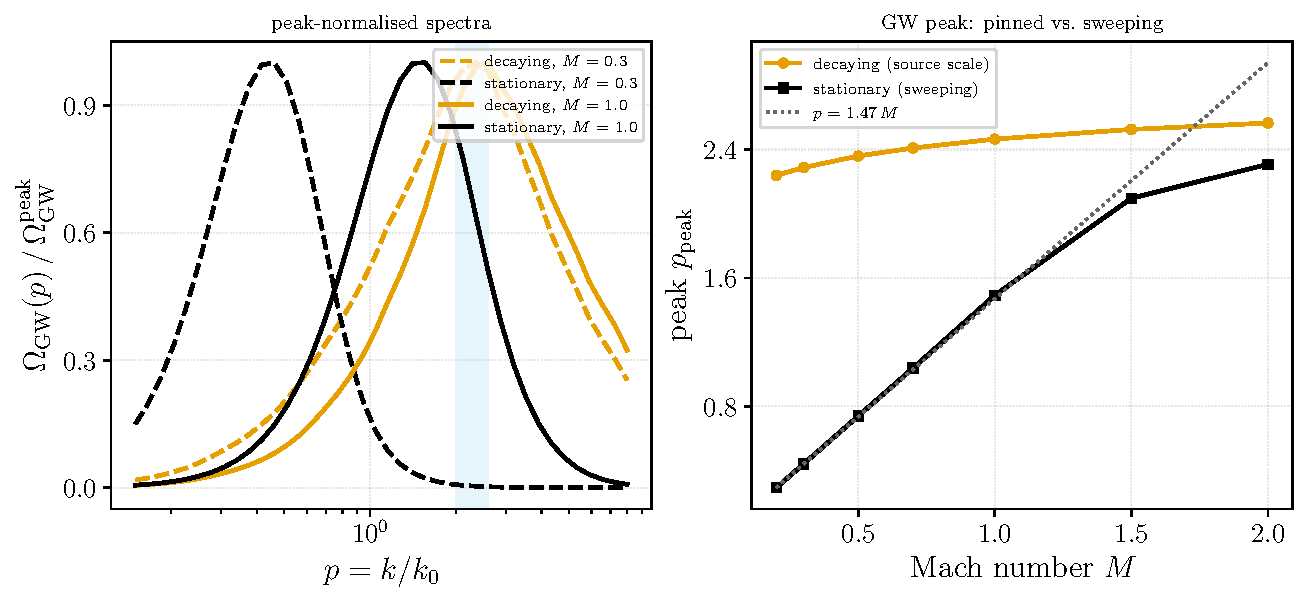
\includegraphics[width=\columnwidth]{fullspatial_decay_peak}
  \caption{The decaying source pins the GW peak at the source scale, in contrast to
  the stationary sweeping peak. (a)~Peak-normalised spectra
  $\Omega_{\rm GW}(p)=p^3H_{ijij}(p,p;M,R)$ ($R=10^4$) for the decaying
  (power-law, orange) and stationary (Gaussian, black) kernels at $M=0.3$ (dashed)
  and $M=1$ (solid): the decaying peaks fall in the source-scale band
  $p\simeq2$--$2.6$ (shaded) for both $M$, whereas the stationary peaks shift with
  $M$. (b)~Peak location versus $M$: the decaying peak is flat at
  $p_{\rm peak}\simeq2.4$ [Eq.~\eqref{eq:decay-peak}], while the stationary peak
  follows $p_{\rm peak}=1.47\,M$ (dotted) until it saturates only as $M\to1$
  (the luminal limit).
  Computed with the full-spatial kernel via the FT-of-product
  Eq.~\eqref{eq:ft-of-product}; generated by
  \texttt{Notebooks/fullspatial\_decay.py}.}
  \label{fig:fullspatial_decay}
\end{figure}

\begin{figure}[ht]
  \centering
  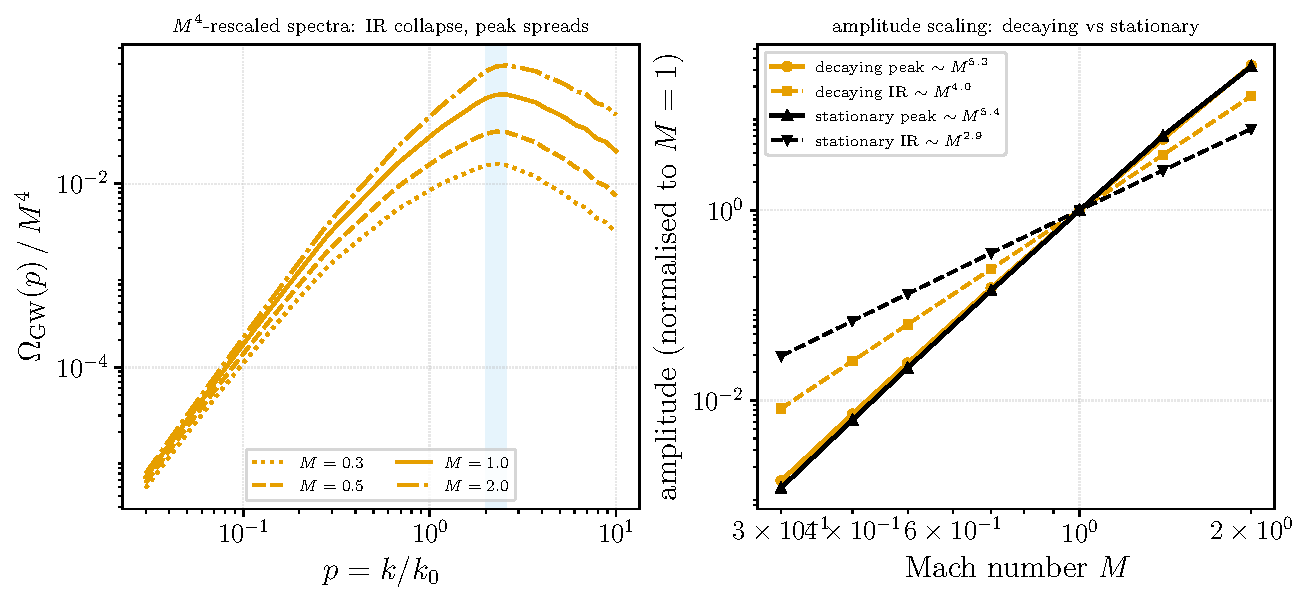
\includegraphics[width=\columnwidth]{decaying_amplitude}
  \caption{Mach scaling of the full-spatial decaying GW amplitude, from the exact
  factorisation $\Omega_{\rm GW}=M^4 p^3\Psi(p,p/M)$ [Eq.~\eqref{eq:decay-amplitude}].
  (a)~$M^4$-rescaled spectra $\Omega_{\rm GW}(p)/M^4$ for $M=0.3$--$2$ ($R=10^4$):
  the curves collapse in the infrared---confirming the $M^4$ prefactor---and spread
  upward through the source-scale band (shaded), the peak amplitude growing faster
  than $M^4$. (b)~Amplitude versus $M$, normalised at $M=1$, with fitted power laws:
  the decaying infrared amplitude scales as $M^{4.0}$ (one power above the stationary
  $M^{2.9}$), while the source-pinned peak amplitude steepens to $M^{5.3}$. Generated
  by \texttt{Notebooks/decaying\_amplitude.py}.}
  \label{fig:decaying_amplitude}
\end{figure}

\subsection{Confrontation with the Roper Pol simulation}
\label{sec:roperpol-compare}

We now test the two pictures against the relativistic MHD turbulence simulation of
Roper Pol et al.~\cite{2019RoperPol} (run ini2), whose fluid and GW spectra (their
Fig.~1) we digitize directly from the published figure by pixel extraction---not by
eyeballed point-reading. The fluid spectrum $\Omega_{\rm M}/k$ shows the expected
Batchelor infrared $k^4$ joined to a Kolmogorov $k^{-5/3}$ inertial range, peaking at
$k_0\simeq673$ in the simulation's units; integrating it gives a turbulent energy
fraction $\Omega_{\rm M}=\int(\Omega_{\rm M}/k)\,dk\simeq1.8\times10^{-3}$, i.e.\ a
deeply subsonic effective Mach number $M\simeq\sqrt{\Omega_{\rm M}}\sim0.05$. Two
features of the simulated GW spectrum discriminate between the sweeping and
source-scale pictures.

\paragraph{Spectral shape.} Figure~\ref{fig:roperpol_comparison} overlays our analytic
$\Omega_{\rm GW}/k=p^2H_{ijij}(p,p)$ for both temporal models on the digitized data.
Each prediction's amplitude is fixed not by a free fit but by the measured energy
fraction---scaled so that its total GW energy equals the simulated
$\Omega_{\rm GW}=(\mathcal H_\ast/k_0)\,\Omega_{\rm M}^2$. Normalised this way the three
curves coincide near the peak, and the simulated ultraviolet slope ($\simeq k^{-11/3}$,
the value reported in \cite{2019RoperPol}) lies \emph{between} the two kernels: the
stationary Gaussian-sweeping kernel is too steep ($\simeq k^{-5.5}$, essentially
$M$-independent across the subsonic range) while the decaying power-law kernel is too
shallow ($\simeq k^{-2.6}$). The physical decorrelation is intermediate between the
rapidly-decorrelating (stationary) and slowly-decorrelating (decaying) limits; neither
idealization alone reproduces the inertial-range slope.

\paragraph{Peak location.} The sharper discriminant is the peak. In the
$\Omega_{\rm GW}=d\rho_{\rm GW}/d\ln k$ convention the simulated GW peak sits at
$k_{\rm peak}\simeq1.84\,k_0$---\emph{above} the source scale, near $2k_0$, the ``twice
the source scale'' value expected when the quadratic stress autocorrelates a source
peaked at $k_0$. Figure~\ref{fig:gw_peak_vs_mach} plots the GW peak against $M$ for both
kernels together with the time-resolved simulation track: because the run is
\emph{decaying}, its Mach number falls with time, and the measured peak stays
pinned at the source scale ($\simeq2.4\,k_0$) as $M(t)$ sweeps down rather than
sliding along the sweeping law---a direct, time-domain discriminant between the
two pictures. The decaying kernel pins the peak at
$p_{\rm peak}\simeq2.4$ for every $M$ and passes through the simulation point; the
stationary sweeping kernel instead gives $p_{\rm peak}\simeq1.47\,M$, which at the
simulation's Mach lies at $\simeq0.07\,k_0$, more than an order of magnitude below both
the source scale and the data. This conclusion is robust to the uncertain effective
Mach: across the \emph{entire} subsonic range $M<1$ the sweeping peak never reaches
$k_0$, whereas the simulated peak---like the decaying kernel---lies above it. The
simulated GW spectrum therefore peaks where the decaying, source-scale picture predicts,
not where the stationary sweeping picture does.

\paragraph{Amplitude and efficiency.} The overall amplitude is a genuine efficiency, not a
free normalisation: the saturated GW energy scales quadratically with the source energy,
$\Omega_{\rm GW}\propto\Omega_{\rm M}^2$, times the square of the dominant length scale, so
that on dimensional grounds $\Omega_{\rm GW}\sim\Omega_{\rm M}^2(\mathcal H_\ast/k_0)^2$ up to
an $\mathcal O(1)$--$\mathcal O(10^2)$ prefactor that depends on the driving. From the run
\texttt{ini2} spectra we measure a dimensionless efficiency
$\Omega_{\rm GW}/\Omega_{\rm M}^2\simeq(2$--$6)\times10^{-5}$ (Fig.~\ref{fig:roperpol_timeseries}b),
consistent with the digitized late-time value $1.7\times10^{-5}$ used to normalise
Fig.~\ref{fig:roperpol_comparison}. Roper Pol et al.\ find the efficiency itself depends
strongly on the driving---forced acoustic and forced magnetic turbulence radiate
$\sim\!200\times$ and $\sim\!10\times$ more than an initially imposed, freely decaying field of
the same energy---and that LISA detectability of electroweak-scale turbulence needs
$\sim0.1$--$10\%$ of the plasma energy in motions or magnetic fields \cite{2019RoperPol}. This
is why the amplitude is set by an energy fraction and a length scale, and why a decaying source
(our and their \texttt{ini2} case) is the least efficient of the drivings.

\paragraph{Steady oscillatory state.} A caveat on what ``the'' spectrum means here. After the
magnetic source decays, GW \emph{production} stops but the modes do not: each GW mode free-rings
at its frequency, so the spectrum shown (theirs and ours) is a \emph{late-time time-average}
over at least one oscillation period, once the energy fluctuates about a steady mean rather than
growing. Our reanalysis makes this concrete
(Fig.~\ref{fig:roperpol_timeseries}b): $\Omega_{\rm GW,tot}$ becomes steady to $\pm4\%$ for
$t>1.15$ while $\Omega_{\rm M,tot}$ is still falling. The stationary and decaying kernels of
this paper both target this time-averaged steady state, not an instantaneous snapshot.

\paragraph{Viscosity.} The simulations run at magnetic Prandtl number $\nu/\eta=1$ and at the
smallest viscosity the resolution allows---far above the physical value---so their Reynolds
number is modest. In our kernels this enters only as the inertial-range width
$R=(k_d/k_0)^{4/3}$, which sets the dissipation cutoff $k_d$ and hence the upper end of the
$k^{-11/3}$ tail; it does \emph{not} set the tail's slope, which is the Kolmogorov inertial-range
value. Consistently, the decaying peak we compute drifts only from $2.40$ to $2.60$ as $R$ runs
over $10^3$--$10^5$ (a dissipation-set peak would scale as $R^{3/4}$), confirming that the peak
and the infrared are viscosity-insensitive and that viscosity is a purely ultraviolet,
dissipation-range effect on the GW spectrum.

\begin{figure}[ht]
  \centering
  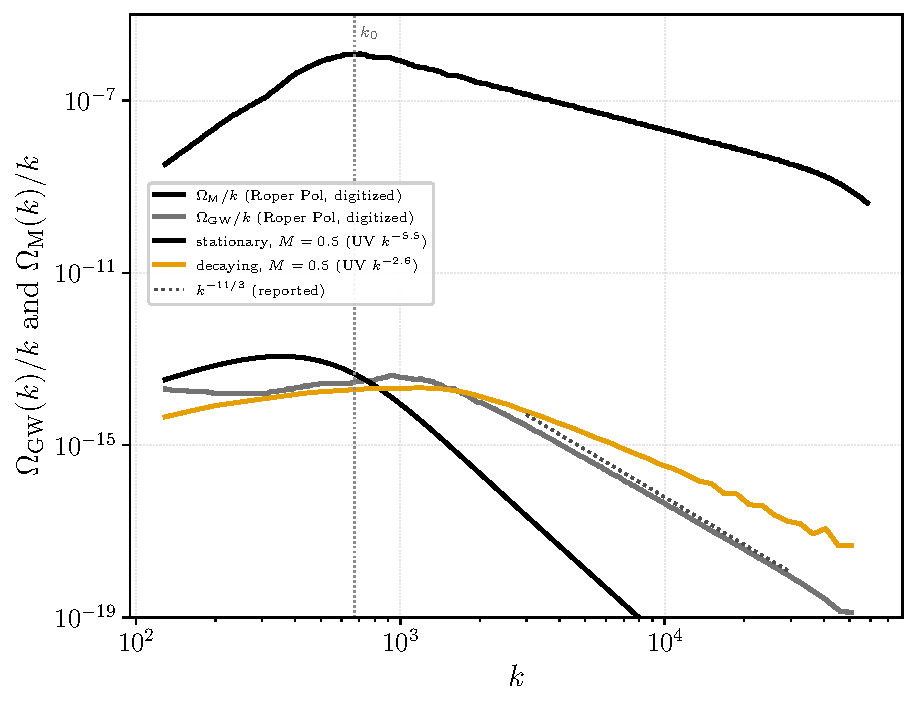
\includegraphics[width=\columnwidth]{roperpol_comparison}
  \caption{Analytic GW spectra confronted with the digitized Roper Pol et
  al.~\cite{2019RoperPol} simulation (their Fig.~1, run ini2; pixel-digitized, no
  fabricated points). Black/grey: digitized fluid $\Omega_{\rm M}/k$ and GW
  $\Omega_{\rm GW}/k$. Orange/thin black: our decaying and stationary
  $\Omega_{\rm GW}/k=p^2H_{ijij}(p,p)$ at $M=0.5$ (the ultraviolet slope is
  $M$-insensitive in the subsonic range), each scaled so its total GW energy matches
  the simulated $\Omega_{\rm GW}=(\mathcal H_\ast/k_0)\Omega_{\rm M}^2$
  (energy-fraction normalisation, no free fit). The simulated UV slope ($\sim k^{-11/3}$,
  dotted) falls between the too-steep stationary and too-shallow decaying kernels; the
  dotted vertical marks the source scale $k_0$. Generated by
  \texttt{Notebooks/roperpol\_comparison.py}.}
  \label{fig:roperpol_comparison}
\end{figure}

\begin{figure}[ht]
  \centering
  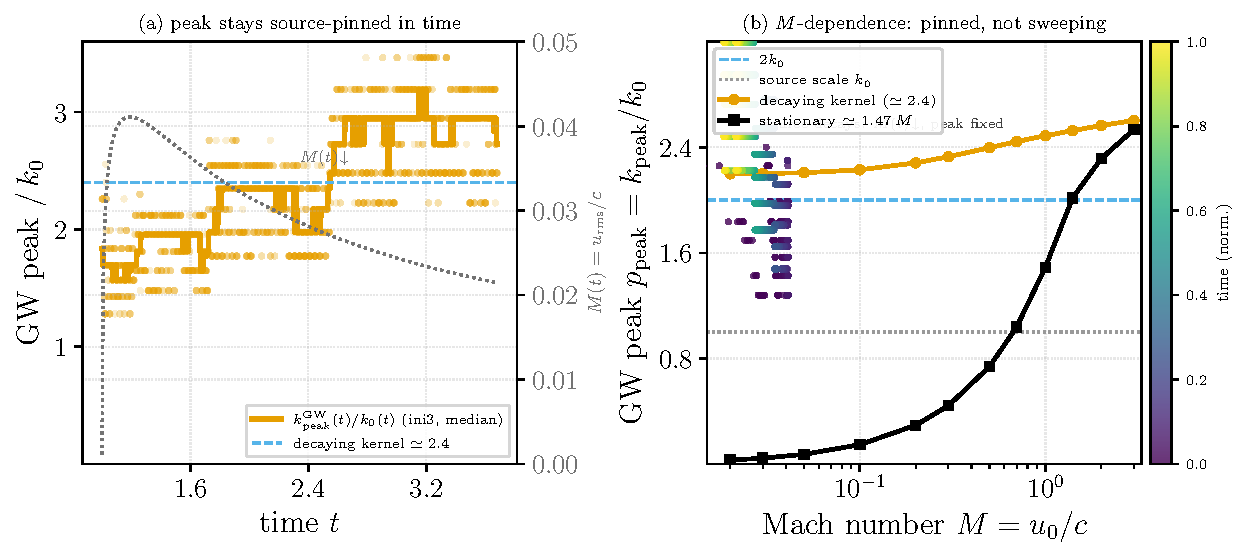
\includegraphics[width=\columnwidth]{gw_peak_vs_mach}
  \caption{The GW spectral peak $k_{\rm peak}/k_0$ (in the $\Omega_{\rm GW}=d\rho/d\ln k$
  convention) \emph{through time} and versus Mach number, from the public
  time-resolved data of the decaying runs \texttt{ini2}/\texttt{ini3}
  \cite{2019RoperPol} (Zenodo 10.5281/zenodo.3692072).
  \emph{(a)}~The peak-to-source ratio $k_{\rm peak}^{\rm GW}(t)/k_0(t)$ (points, with
  a running median) holds at the source-scale value $\simeq2.4$ (dashed) throughout
  the run, while the instantaneous Mach number $M(t)=u_{\rm rms}(t)/c$ (dotted, right
  axis) rises after switch-on and then \emph{decays}; the absolute peak $k_{\rm peak}$
  and $k_0$ both drift down together (helical inverse transfer), but their ratio is
  fixed. The scatter is the discrete-shell wavenumber resolution
  ($k_0$ at shells $\sim4$--$7$).
  \emph{(b)}~The same peak versus $M$: analytic decaying (source-scale, $\simeq2.4$)
  and stationary (sweeping, $\simeq1.47\,M$) kernels, with the simulation
  \emph{time-track} (points coloured by time) superposed. As the source decays the
  Mach number sweeps down through $M(t)\simeq0.04\to0.02$, yet the peak stays on the
  decaying branch at $\simeq2.4\,k_0$---roughly two orders of magnitude above the
  sweeping prediction ($1.47M\sim0.03$) at the same $M$. The time evolution therefore
  discriminates the two pictures directly: a sweeping peak would slide \emph{down} the
  black curve as $M(t)$ falls, whereas the simulated peak does not move.
  Generated by \texttt{Notebooks/gw\_peak\_vs\_mach.py}.}
  \label{fig:gw_peak_vs_mach}
\end{figure}

\section{The principal simulation--analytic discrepancy}
\label{sec:principal-discrepancy}

Setting the two analytic treatments in the literature---the stationary Kraichnan--K41
model of Gogoberidze et al.~\cite{2007Gogoberidze} and the helical inverse-cascade model
of Kahniashvili et al.~\cite{2008Kahniashvili}---beside the direct simulations of
Roper Pol et al.~\cite{2019RoperPol} isolates one discrepancy that is both physically
significant and shared by \emph{every} analytic estimate, the kernels of this paper
included. It concerns not the location of the peak (Sec.~\ref{sec:peak-location}) but the
slope of the spectrum \emph{below} the peak.

\paragraph{Three temporal pictures, three peaks.} The analytic works differ in how they
model the source's unequal-time correlation, and that choice fixes their spectra. Both
\cite{2007Gogoberidze} and the direct-cascade stage of \cite{2008Kahniashvili} adopt a
Gaussian decorrelation $f(\tau)=\exp(-\tfrac{\pi}{4}\eta_k^2\tau^2)$ with the eddy-turnover
rate $\eta_k\propto\varepsilon^{1/3}k^{2/3}$, which radiates predominantly at the turnover
frequency and places the GW peak near $\omega\sim Mk_0$, below the source scale for subsonic
turbulence. Kahniashvili et al.\ add a second, dominant contribution from the helical
\emph{inverse} cascade: because magnetic helicity is conserved the energy-carrying eddy
grows, and requiring its cascade time to reach the Hubble time drives the dominant peak down
to the Hubble frequency $f_H\simeq1.6\times10^{-5}\,$Hz, essentially independent of the
cascade model. The simulations \cite{2019RoperPol} make no closure assumption---the source
is freely decaying MHD turbulence---and find the GW peak at $k_{\rm GW}\simeq2k_0$, twice the
field scale, the elementary consequence of the source being the \emph{quadratic} stress
$T_{ij}\sim B_iB_j$ whose spectrum peaks at twice the field peak. These three pictures place
the GW peak at $Mk_0$, at $f_H$, and at $2k_0$ respectively---spanning orders of magnitude
(Table~\ref{tab:three-works}); the $2k_0$ result is the one borne out in
Sec.~\ref{sec:roperpol-compare}.

\paragraph{The discrepancy: $k^3$ versus $k$.} Beneath the peak the disagreement is sharper
and universal. Every \emph{quasi-stationary} analytic treatment---the aeroacoustic
Gaussian-closure framework of \cite{2007Gogoberidze,2008Kahniashvili} and both the stationary
and decaying single-emission-epoch kernels of this paper---gives the \emph{causal} infrared
slope
\begin{equation}
  \Omega_{\rm GW}(k)\;\propto\;k^3 \qquad (k<k_{\rm peak}),
  \label{eq:ir-causal}
\end{equation}
which follows from the analyticity of the equal-time stress correlator at $k\to0$. The
simulations instead find the far shallower
\begin{equation}
  \Omega_{\rm GW}(k)\;\propto\;k^1 \qquad (k<k_{\rm peak}),
  \label{eq:ir-sim}
\end{equation}
i.e.\ a \emph{flat} $\Omega_{\rm GW}(k)/k$. Roper Pol et al.\ single this out as their central
new result---``the subinertial power law $\Omega_{\rm GW}\sim k$ is a novel result from our
simulations that was not obtained in previous analytical estimates''---their Table~II
contrasting the analytic infrared slope $3$ with the simulated slope $1$ for the \emph{same}
magnetic spectrum $\Omega_{\rm M}\propto k^5$. Our own digitization of their Fig.~1
(Sec.~\ref{sec:roperpol-compare}) confirms it: the measured GW infrared slope is
$\simeq k^{+1.3}$, not $k^3$ [Fig.~\ref{fig:roperpol_comparison}].

\paragraph{Why it is significant.} The discrepancy is two infrared powers of $k$, and it
flips the sign of the strain slope: $h_c(f)\propto f^{+1/2}$ in the analytic estimates versus
$f^{-1/2}$ in the simulations. Because the peak sits near the high-frequency end of the
accessible band, this shallower-than-causal slope governs the \emph{entire} sub-peak
range---most of the observational band for an electroweak-scale source---so it changes the
predicted low-frequency power, and hence the detectability, in the opposite direction to what
the causal estimates assume.

\paragraph{What finite duration can and cannot do.} The causal $k^3$ of
Eq.~\eqref{eq:ir-causal} is the strict $k\to0$ asymptote and is unavoidable: the equal-time
stress of a spatially compact source is analytic (white) at $k\to0$, and our quasi-stationary
kernels reproduce it (measured infrared slope $2.93$ over $p=10^{-3}$--$10^{-2}$). Could the
\emph{finite duration} of the source nonetheless open a shallower band above this asymptote?
Carrying the unequal-time integration over a finite emission window $[0,T_{\rm em}]$ replaces
the stationary frequency factor by the finite-duration kernel
\begin{equation}
  \int_0^{T_{\rm em}}\!\!\!\int_0^{T_{\rm em}}\!\! dt_1\,dt_2\;e^{i\omega(t_1-t_2)}
  \;\longrightarrow\;\frac{4\sin^2(\omega T_{\rm em}/2)}{\omega^2}
  \;\xrightarrow[\;\rm ens.\,avg\;]{\;\omega T_{\rm em}\gg1\;}\;\frac{2}{\omega^2},
  \label{eq:duration-kernel}
\end{equation}
which tends to $T_{\rm em}^2$ (a constant, giving $k^3$) for $\omega T_{\rm em}\ll1$ but to
$2/\omega^2$ (giving $k^1$) for $\omega T_{\rm em}\gg1$---\emph{provided the source stays
coherent across the window}. A source that is both coherent and sustained over
$[0,T_{\rm em}]$ would thus carry a $k^1$ sub-peak band; this is the regime in which a source
treated as statistically stationary over a finite duration reproduces the simulated slope.

\paragraph{Freely decaying turbulence does not realise it.} Self-similar decaying turbulence
fails the coherent-\emph{and}-sustained condition. Its correlation time is the eddy-turnover
(sweeping) time $\tau_c(k)=1/(\varepsilon^{1/3}k^{2/3})\propto1/(Mk^{2/3})$, fixed by the
velocity and \emph{independent} of the decay time; Kolmogorov consistency
($\varepsilon\sim u^3/L\sim u^2/\tau_{\rm st}$) ties the decay time to the outer-scale eddy
turnover, $\tau_{\rm st}\sim L/u$, so the dimensionless decay rate
$\varepsilon_0=\tau_{\rm eddy}/\tau_{\rm st}$ is of order unity, not a free parameter. As the
flow decays the eddy time grows, but the source amplitude falls faster
($\Phi_{\rm eq}\propto(1+t/\tau_{\rm st})^{-34/21}$ per leg), so the eddies turn coherent only
\emph{after} they have decayed away: the growing coherence is cancelled by the decaying
amplitude, and the coherent, sustained window required for $k^1$ is never reached for sub-peak
modes. We verify this with a first-principles full-spatial self-similar kernel---the geometry
of Sec.~\ref{sec:decaying-peak} with the temporal factor replaced by the genuine slow-time
double-time integral over $[0,T_{\rm em}]$, which reduces to the quasi-stationary kernel as
$T_{\rm em}\to\infty$ (cross-check ratio $\to1$). Its infrared slope is causal ($\simeq2.5$,
steepening to $3$ as $p\to0$) and essentially \emph{independent of the decay rate}---$2.53$,
$2.57$, $2.51$ for $\varepsilon_0=0,\,1,\,4$ [Fig.~\ref{fig:ir_resolution}]. The finite
duration of a decaying source does not flatten the infrared.

\paragraph{Roper Pol's own explanation, and a time-domain reconciliation.}
Before attributing the $k^1$ to physics missing from our kernels, it is worth taking
seriously the explanation given by \cite{2019RoperPol} themselves, which is both simpler
and---as we verify below---correct. They observe that the GW source is the \emph{quadratic}
magnetic stress $\sim B_iB_j$, and that the spectrum of $B^2$ ``can never be steeper than
that of white noise'': a causal (Batchelor) magnetic field with $E_M\propto k^4$ produces a
stress spectrum that flattens to $E_T\propto k^2$ at large scales, and the GW spectrum
inherits this white-noise ceiling rather than the naive causal $k^3$. This is the same
convolution mechanism that makes our own white-noise model
(Sec.~\ref{sec:white}, $E\propto k^2$) analytic in the infrared, read one power of $k$
shallower.

Crucially, \cite{2019RoperPol} add that the causal $k^3$ is not absent but \emph{transient}:
a flat spectrum reaching arbitrarily large scales would be acausal, so at the very largest
scales and earliest times the spectrum grows as $k^3$ before saturating to the flat $k^1$
plateau, and this transition ``is much shorter than the time it takes for the GW spectrum to
become stationary.'' We confirm this directly by reanalysing the public time-resolved spectra
of their run \texttt{ini2} (Fig.~\ref{fig:roperpol_timeseries}; data from
\cite{2019RoperPol} via Zenodo). At source switch-on the infrared slope is the causal
$\Omega_{\rm GW}\sim k^{3}$ (measured $k^{3.3}$ at $t=1.00$), and within $\Delta t\sim0.02$
it flattens to the saturated $\Omega_{\rm GW}\sim k^{1}$ shown in the paper's Fig.~1. The
total GW energy then fluctuates about a constant mean---the ``steady oscillatory state'' of
the freely ringing GW field---while the magnetic energy keeps decaying; and the magnetic
peak $k_0(t)$ migrates to smaller $k$, the signature of the helical inverse transfer.

\paragraph{What the discrepancy points to.} This reframes the tension considerably. The
causal $k^3$ of our quasi-stationary and self-similar kernels is not contradicted by the
simulation: it is the early-time transient, and the discrepancy with the simulated $k^1$ is a
comparison of an \emph{asymptotic} analytic slope with a \emph{time-saturated} simulated one
(the same axis mismatch anticipated for the finite-window band, Sec.~\ref{sec:cps-reproduction}).
Two ingredients set the saturated slope---the white-noise ceiling of the quadratic stress, and
the sustained coherence of the inverse-transferred magnetic field visible in
Fig.~\ref{fig:roperpol_timeseries}---neither of which is captured by a single-time
hydrodynamic kernel. The honest statement is therefore weaker than a genuine failure of
causality and stronger than a mere convention: our kernels give the correct transient
infrared, and reproducing the stationary $k^1$ requires following the source through its
saturation, a target for a dedicated time-dependent MHD calculation.

\begin{figure}[ht]
  \centering
  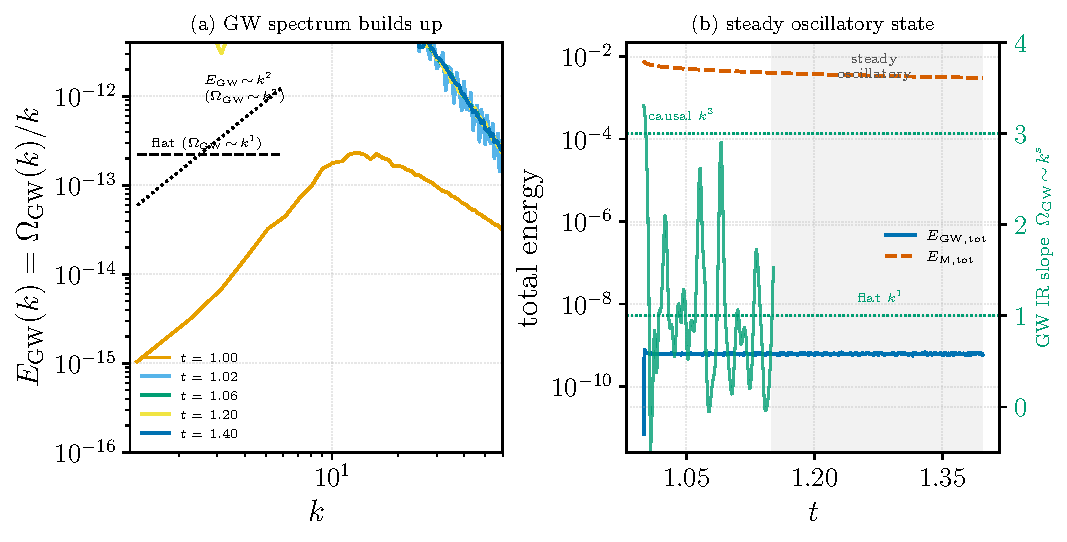
\includegraphics[width=\columnwidth]{roperpol_timeseries}
  \caption{Time-series reanalysis of the Roper Pol et al.~\cite{2019RoperPol} run
  \texttt{ini2} (public Pencil Code spectra, Zenodo 10.5281/zenodo.3692072), the run of their
  Fig.~1. \emph{(a)}~The GW energy spectrum $E_{\rm GW}=\Omega_{\rm GW}/k$ at successive times:
  at switch-on ($t\simeq1.0$) the infrared follows the causal $E_{\rm GW}\sim k^2$
  ($\Omega_{\rm GW}\sim k^3$) and within $\Delta t\sim0.02$ saturates to the flat plateau
  ($\Omega_{\rm GW}\sim k^1$) of their Fig.~1. \emph{(b)}~Total energies versus time: the GW
  energy rises while the source acts, then fluctuates about a steady mean (grey band; the
  ``steady oscillatory state''), while the magnetic energy keeps decaying; the right axis (green)
  shows the measured GW infrared slope crossing from the causal $k^3$ to the saturated $k^1$.
  Generated by \texttt{Notebooks/roperpol\_timeseries.py}, which auto-downloads the data.}
  \label{fig:roperpol_timeseries}
\end{figure}

\begin{figure}[ht]
  \centering
  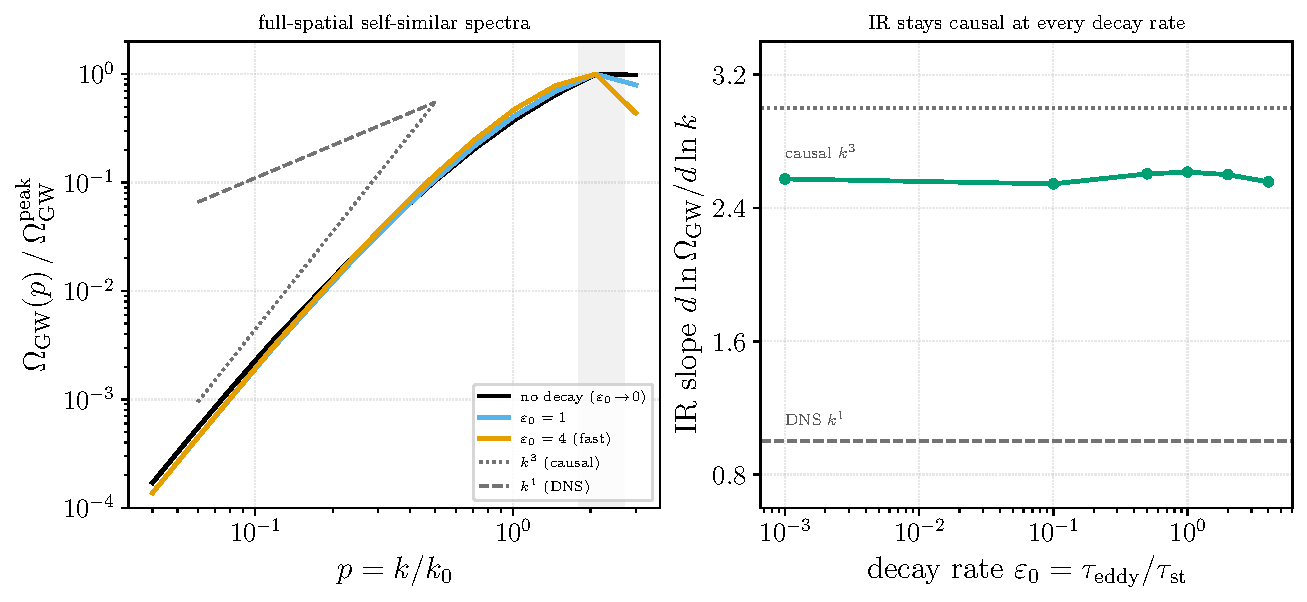
\includegraphics[width=\columnwidth]{fullspatial_selfsimilar_exact}
  \caption{The finite duration of a \emph{decaying} source does not flatten the infrared.
  \emph{Left:} GW spectra from the first-principles full-spatial self-similar kernel
  ($T_{\rm em}=40\,\tau_{e0}$, $M=1$) at three decay rates; the infrared slopes overlap on the
  causal $k^3$ guide (dotted) rather than the $k^1$ guide (dashed), and share the source-scale
  peak (shaded). \emph{Right:} the infrared slope versus the decay rate
  $\varepsilon_0=\tau_{\rm eddy}/\tau_{\rm st}$ stays at the causal value ($\simeq2.5$--$3$)
  for every $\varepsilon_0$, never approaching the simulated $k^1$; the physically realised
  self-similar decay sits at $\varepsilon_0\sim1$. Generated by
  \texttt{Notebooks/fullspatial\_selfsimilar\_exact.py}.}
  \label{fig:ir_resolution}
\end{figure}

\begin{table*}[ht]
  \centering
  \begin{tabular}{l l l l l}
    \hline\hline
    treatment & temporal decorrelation & GW peak & infrared $\Omega_{\rm GW}$ & high-$k$ $\Omega_{\rm GW}$ \\
    \hline
    Gogoberidze 2007 \cite{2007Gogoberidze} & Gaussian, $\eta_k\propto k^{2/3}$  & $\sim M k_0$  & $k^3$ & steep ($\sim k^{-7/2}$) \\
    Kahniashvili 2008 \cite{2008Kahniashvili} & Gaussian $+$ helical inverse cascade & $\to f_H$ (Hubble scale) & $k^3$  & Kolmogorov input \\
    this paper  & Gaussian / power-law / self-similar decay & $1.47Mk_0$ / $2.4k_0$ & $k^3$ (causal)  & $k^{-5}$ / $k^{-8/3}$ \\
    Roper Pol 2020 \cite{2019RoperPol} & freely decaying & $2k_0$ & $k^1$ & $k^{-8/3}$ \\
    \hline\hline
  \end{tabular}
  \caption{Temporal-decorrelation assumption, GW spectral peak, and spectral slopes for the
  three literature treatments and the kernels of this paper. The peak frequency spans orders
  of magnitude across the three works; the infrared slope is the discrepancy that is
  universal across \emph{every} analytic treatment---the quasi-stationary estimates
  \emph{and} the first-principles self-similar decaying kernel of this paper all give the
  causal $k^3$ (Fig.~\ref{fig:ir_resolution})---yet is contradicted by the simulation
  ($k^1$). Restoring the finite duration of a freely decaying source does \emph{not} flatten
  the infrared: the growing eddy coherence is cancelled by the faster amplitude decay, so the
  hydrodynamic infrared stays causal for every decay rate. The tension is therefore genuine
  and localizes to physics absent from this hydrodynamic description (Sec.~\ref{sec:principal-discrepancy}).
  The infrared slope is not quoted explicitly by
  \cite{2008Kahniashvili} but is the generic causal value of their aeroacoustic
  Gaussian-closure framework. Slopes are in the $\Omega_{\rm GW}=d\rho_{\rm GW}/d\ln k$
  convention.}
  \label{tab:three-works}
\end{table*}

\subsection{Reproduction of the universal infrared theorem}
\label{sec:cps-reproduction}

The causal $k^{3}$ invoked repeatedly above is not a property of our kernels but a
theorem. Cai, Pi and Sasaki~\cite{2020CaiPiSasaki} prove that
$\Omega_{\rm GW}\propto k^{3}$ in the infrared for any source satisfying
\begin{enumerate}\itemsep0pt
  \item[(I)] $0<\int d\ell\,[\text{source spectra}]^{2}<\infty$ (finiteness);
  \item[(II)] $k$ lies below \emph{every} scale associated with the source---its peak
    $k_{*}$, its spectral width $\Delta k$, \emph{and} the inverse duration
    $\Delta t_{s}^{-1}=(a_{*}\Delta\eta_{s})^{-1}$;
  \item[(III)] the modes re-enter the horizon during radiation domination.
\end{enumerate}
The exponent itself is pure counting: at horizon crossing of $1/k_{*}$ there are
$N=(k_{*}/k)^{3}$ causally disconnected patches, so Poisson statistics give
$\langle h_{k}h_{k}\rangle=N^{-1}|h_{*}|^{2}=(k/k_{*})^{3}|h_{*}|^{2}$, and the $k^{3}$
follows from the dimensionality of space alone, independently of the later evolution.

This matters here because \emph{both} of the exceptions they identify are realised by
models in this paper, so the theorem is an external check rather than a restatement of
our own kernels. We therefore reproduce it directly, from scratch and independently of
Sec.~\ref{sec:monochromatic-white} (Fig.~\ref{fig:cps-reproduction}).

\paragraph{Spectral width, and why a monochromatic source gives $k^{2}$.}
The anisotropic stress is the convolution of two source shells, which in one dimension
carries an explicit pole,
\begin{equation}
  \Pi(k)=\frac{2\pi}{k}\int\!dp\,p\,P(p)\!\int_{|k-p|}^{k+p}\!\!dq\,q\,P(q).
  \label{eq:stress-convolution-1d}
\end{equation}
For a source of finite width the inner interval shrinks as $2k$ when $k\to0$, cancelling
the $1/k$ and leaving $\Pi(0)$ finite, so $\Omega_{\rm GW}\propto k^{3}$. For a
$\delta$-shell the inner integral does not shrink; the pole survives, and
$\Omega_{\rm GW}\propto k^{3}\cdot k^{-1}=k^{2}$. Numerically, a shell of log-width
$\sigma$ gives slope $3.000$ for $k\ll\sigma$ and $2.000$ in the unscreened band
$\sigma\ll k\ll k_{*}$ (measured for $\sigma=10^{-2}$ and $10^{-3}$), while an exact
$\delta$-shell gives $2.000$ over the whole infrared---a zero-width source has no lower
scale, which is precisely the violation of condition~(II). This is the same $1/p$ pole
that appears in our monochromatic kernel as $\mathcal{K}_{0}(p)/p$, and it is why both
panels of Fig.~\ref{fig:spectrum_delta_k_pair} show slope $\mathbf{2}$ rather than
$\mathbf{3}$: the monochromatic models are Cai--Pi--Sasaki's $\delta$-function exception,
not an anomaly of our temporal treatment.

\paragraph{Duration, and the intermediate $k^{1}$ band.}
Condition~(II) also bounds $k$ by the inverse duration. For a source coherent over a
window $\Delta\eta$ the temporal factor is
\begin{equation}
  \Bigl|\int_{0}^{\Delta\eta}\!d\eta\,e^{ik\eta}\Bigr|^{2}
  =\frac{4\sin^{2}(k\Delta\eta/2)}{k^{2}}
  \;\longrightarrow\;
  \begin{cases}
    \Delta\eta^{2}, & k\Delta\eta\ll1,\\[2pt]
    2/k^{2}, & k\Delta\eta\gg1\ \text{(oscillation-averaged)},
  \end{cases}
  \label{eq:window-factor}
\end{equation}
so the spectrum measures slope $+2.999$ below $1/\Delta\eta$ and exactly $+1.000$ above
it: the finite emission window removes two powers. The $k^{1}$ that appears at
intermediate wavenumbers is therefore not a violation of causality but condition~(II)
being read outside its domain---$k^{3}$ is the asymptotic law for $k\ll1/\Delta\eta$,
and $k^{1}$ is the finite-window band above it. (Cai--Pi--Sasaki quote $k^{9}$ above
$1/\Delta\eta$ for acoustic sources, where a coherent \emph{oscillating} source resonates
with the Green function; for an incoherent window such as ours the loss is two powers.)

\begin{figure}[ht]
  \centering
  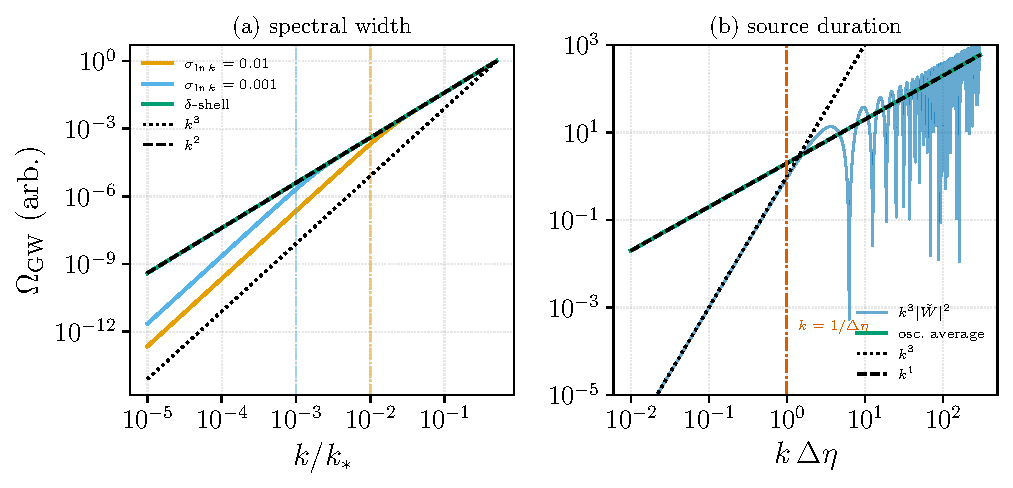
\includegraphics[width=\textwidth]{cai_pi_sasaki_reproduction}
  \caption{Independent reproduction of the two exceptions to the universal $k^{3}$
  infrared theorem of \cite{2020CaiPiSasaki}, computed from
  Eqs.~\eqref{eq:stress-convolution-1d} and \eqref{eq:window-factor} with no input from
  the kernels of this paper. \emph{(a)} Shells of log-width $\sigma_{\ln k}=10^{-2}$ and
  $10^{-3}$ (dash-dotted verticals mark $k=\sigma$) against an exact $\delta$-shell: the
  finite-width curves follow $k^{3}$ for $k\ll\sigma$ and $k^{2}$ in the band
  $\sigma\ll k\ll k_{*}$, while the $\delta$-shell follows $k^{2}$ throughout, having no
  lower scale. \emph{(b)} Finite emission window $\Delta\eta$: the spectrum follows
  $k^{3}$ below $k=1/\Delta\eta$ and, once the $\sin^{2}$ oscillations are averaged,
  $k^{1}$ above. Measured slopes are $3.000/2.000$ and $2.999/1.000$ respectively.
  Generated by \texttt{Notebooks/cai\_pi\_sasaki\_reproduction.py}.}
  \label{fig:cps-reproduction}
\end{figure}

\section{Monochromatic and White-Noise Spectra}
\label{sec:monochromatic-white}

We now consider two alternative models for the turbulence power spectrum and carry out the same GW-kernel derivation in each case. The first model replaces the Kolmogorov spectrum by a monochromatic (delta-function) distribution in wavenumber; the second takes the real-space two-point function to be spatially uncorrelated (delta function in $\br$), which corresponds to a flat (white-noise) spectrum in $k$-space. For each spatial model we work out both the Kraichnan stationary decorrelation and the decaying-turbulence temporal model, giving four cases in total.

The derivation follows the same sequence of steps as in Sec.~\ref{sec:kraichnan-k41}: (i) write $H_{ijij}$ as a double convolution in both $\kb$ and $\omega$, (ii) insert the spectral model, (iii) perform the tensor contractions to get $\mathcal{K}$, (iv) switch to spherical coordinates and the variable $u=|\kb-\kb_1|$, (v) evaluate or simplify the temporal integral, and (vi) introduce dimensionless variables.

\subsection{\texorpdfstring{Monochromatic energy spectrum $E(k)=E_0\delta(k-k_0)$}{Monochromatic energy spectrum E(k)=E0 delta(k-k0)}}
\label{sec:delta-k}

Set $E(k)=E_0\,\delta(k-k_0)$ so that $A(k) = E_0\,\delta(k-k_0)/(4\pi k^2)$ and the spectral tensor reads
\begin{equation}
  \tilde{F}_{ij}(\kb,\omega) = \frac{E_0\,\delta(k-k_0)}{4\pi k^2}\,P_{ij}(\khat)\,\tf(\omega),
  \qquad \int_0^\infty E(k)\,dk = E_0,
  \label{eq:Fij-delta-k}
\end{equation}
with $\tf(\omega)$ to be specified by the decorrelation model.

Starting from Eq.~\eqref{eq: H-with-P} in spherical coordinates, the radial integral collapses $k_1\to k_0$ via $\delta(k_1-k_0)$, fixing $u=\sqrt{k^2+k_0^2-2kk_0\mu}$. Trading $\mu$ for $u$ (azimuth contributes $2\pi$) and using $\delta(u-k_0)$ from $A(u)$ yields the closed-form spatial reduction
\begin{equation}
  2\pi\!\int_{-1}^{1}\!d\mu\,A(u) = \frac{E_0}{2k k_0^2}\,\Theta(2k_0-k),
  \label{eq:angular-delta}
\end{equation}
with the Heaviside factor enforcing the triangle inequality $p \equiv k/k_0 \leq 2$. The geometric kernel at $k_1=u=k_0$ evaluates to
\begin{equation}
  \mathcal{K}_0(p) \equiv \mathcal{K}(k,k_0,k_0) = \frac{14}{3} - \frac{p^2}{3} + \frac{p^4}{12}.
  \label{eq:K0}
\end{equation}
% FLAG: 4 pi error in the dimensional prefactor below.
% int d^3 k_1 A(k_1) A(u) K should give E_0^2 K_0(p) Theta(2-p) / (8 pi k k_0^2).
% Displayed form below has 1/2 in place of 1/(8 pi) — 4 pi too large. The error
% propagates through to Eq.~\eqref{eq:H-delta-Kraichnan} (overall 8 pi too
% large). The boxed mathfrak{H} is unaffected (shape only).
Substituting Eqs.~\eqref{eq:angular-delta}--\eqref{eq:K0} in Eq.~\eqref{eq: H-with-P},
\begin{equation}
  H_{ijij}(\kb,\omega)
  = \frac{E_0^2\,\Theta(2k_0-k)}{2(2\pi)^8\,k k_0^2}\;\mathcal{K}_0(p)\;I_\omega(\omega),
  \qquad
  I_\omega(\omega)\equiv\!\int\!d\omega_1\,\tf(\omega_1)\tf(\omega-\omega_1).
  \label{eq:H-delta-k}
\end{equation}
All spatial structure has been resolved in closed form; only the temporal convolution $I_\omega$ remains. Because both wavevectors are pinned to $k_0$ by the two $\delta$-functions, there is no leftover wavenumber integration: the only spatial constraint is the $M$-independent triangle inequality $\Theta(2-p)$. The Mach number therefore cannot reshape any spatial integration \emph{bounds} here; it enters solely through the temporal decorrelation rate at the fixed scale $k_0$, which we tie to $M$ via $\eta_{k_0}=\tfrac{M}{\sqrt{2\pi}}k_0$ (cf.\ Eq.~\eqref{eq:appA-dimless}). This contrasts with the white-noise case of Sec.~\ref{sec:white}, where $M$ does enter the surviving wavenumber integral.

\subsubsection{Kraichnan decorrelation}
\label{sec:delta-kraichnan}

For $\tf(\omega)=(2/\eta_0)e^{-\omega^2/\pi\eta_0^2}$ with $\eta_0\equiv\eta_{k_0}=M k_0/\sqrt{2\pi}$, the Gaussian convolution gives $I_\omega(\omega) = (2\sqrt{2}\pi/\eta_0)e^{-\omega^2/(2\pi\eta_0^2)}$. With $q\equiv\omega/k_0$ the exponent becomes $\omega^2/(2\pi\eta_0^2)=q^2/M^2$, so Eq.~\eqref{eq:H-delta-k} separates into a dimensional prefactor and the boxed dimensionless kernel
\begin{equation}
  H_{ijij}(\kb,\omega) = \frac{\sqrt{2}\,E_0^2}{(2\pi)^7\,k k_0^2\,\eta_0}\,\mathcal{K}_0(p)\,\Theta(2-p)\,e^{-q^2/M^2},
  \qquad
  \boxed{
  H[S_{\delta k},T_{\rm sw}](p,q;M)\;\equiv\;\mathfrak{H}^{(\delta k)}_{\rm Kraichnan}(p,q;M) = \frac{\mathcal{K}_0(p)}{p}\,\Theta(2-p)\,e^{-q^2/M^2}.
  }
  \label{eq:dimless-delta-Kraichnan}
\end{equation}
There is no remaining integral. The $p$-shape is fixed; $M$ acts only as the Gaussian width in $q$, so the GW spectrum peaks at $q\sim M$.

\subsubsection{Decay model}
\label{sec:delta-decay}

For decaying turbulence, $\tf(\omega)=\hat g(\omega\tau_1)$ with $\hat g(\bar q)=e^{-i\bar q}(-i\bar q)^{-1/3}\Gamma(\tfrac{1}{3},-i\bar q)$ and $\tau_1=1/\eta_0=\sqrt{2\pi}/(M k_0)$ the decay time at scale $k_0$. With $q=\omega/k_0$ the natural temporal argument is $\bar q\equiv\omega\tau_1=\sqrt{2\pi}\,q/M$; changing variables in Eq.~\eqref{eq:H-delta-k}, the temporal factor becomes $I_\omega=(1/\tau_1)\!\int dq_1\,\mathrm{Re}\bigl[\hat g(q_1)\hat g(\bar q-q_1)\bigr]$. The real part is essential and not cosmetic: the convolution is genuinely complex (its imaginary part exceeds its real part already at $\bar q\simeq1$), and it is the real part that carries the spectrum. The dimensionless result is
\begin{equation}
  \boxed{
  H[S_{\delta k},T_{\rm dec}](p,q;M)\;\equiv\;\mathfrak{H}^{(\delta k)}_{\rm decay}(p,q;M) = \frac{\mathcal{K}_0(p)}{p}\,\Theta(2-p)\,\int_{-\infty}^\infty\!dq_1\,\mathrm{Re}\bigl[\hat g(q_1)\,\hat g(\bar q-q_1)\bigr],
  \qquad \bar q=\frac{\sqrt{2\pi}\,q}{M}.
  }
  \label{eq:dimless-delta-decay}
\end{equation}
The spatial part is fully resolved by the two $\delta$-functions; only a 1-D frequency integral remains, and $M$ enters it solely through the rescaled frequency $\bar q$.

\paragraph{The frequency convolution in closed form.}
Contrary to what the singular appearance of $\hat g$ suggests, this convolution
\emph{does} have a closed form, and evaluating it as a written $q_1$ integral is
both unnecessary and numerically treacherous. The GW source is quadratic in the
velocity, so under quasi-normal closure the object the spectrum needs is the
transform of the \emph{squared} two-time correlation,
\begin{equation}
  \mathcal{C}(\bar q)\;\equiv\;\int_{-\infty}^{\infty}\!d\tau\,\cos(\bar q\tau)\,
  \bigl[(1+|\tau|)^{-2/3}\bigr]^{2}
  \;=\;2\,\mathrm{Re}\Bigl[e^{-i\bar q}(-i\bar q)^{1/3}\,
        \Gamma\bigl(-\tfrac13,-i\bar q\bigr)\Bigr],
  \label{eq:cosT-closed}
\end{equation}
which is the \emph{same} closed form as $\hat g$ with the power $2/3\to4/3$ --- squaring
the correlation simply shifts the exponent. Writing $h=f\Theta$ for the one-sided
correlation $f(s)=(1+s)^{-2/3}$, the convolution theorem gives $(\hat g*\hat g)(\bar q)=2\pi\,\mathcal{F}[h^{2}](\bar q)$,
whose real part halves into the one-sided cosine integral. Hence the exact identity
\begin{equation}
  \int_{-\infty}^{\infty}\!dq_1\,\mathrm{Re}\bigl[\hat g(q_1)\hat g(\bar q-q_1)\bigr]
  \;=\;\pi\,\mathcal{C}(\bar q).
  \label{eq:conv-equals-cosT}
\end{equation}
Two consequences are worth stating explicitly. First, the one-sided/two-sided
bookkeeping that distinguishes $\hat g$ from the two-sided kernel enters only as the
constant $\pi$: it carries \emph{no} shape information and therefore cannot bend a
spectral slope. Second, the limits of $\mathcal{C}$ are elementary,
\begin{equation}
  \mathcal{C}(0)=6,
  \qquad
  \mathcal{C}(\bar q)\xrightarrow[\bar q\to0]{}6-3\sqrt{3}\,\Gamma(\tfrac23)\,\bar q^{\,1/3},
  \qquad
  \mathcal{C}(\bar q)\xrightarrow[\bar q\to\infty]{}\frac{8}{3\bar q^{\,2}},
  \label{eq:cosT-limits}
\end{equation}
the last following from the cusp of $f^{2}$ at $\tau=0$. This $\bar q^{-2}$ ultraviolet
tail is the physically decisive one: it is a \emph{heavy power law}, in contrast to the
Gaussian cutoff of the stationary Kraichnan model, and it is what allows the decaying
GW spectrum to extend past the sweeping cutoff so that its peak is pinned at the source
scale (Sec.~\ref{sec:mach-discussion}).

\subsection{Real-space delta-function correlations}
\label{sec:white}

Take the spatial part of $R_{ij}$ to be a $\delta^{(3)}(\br)$, with velocity variance $v_0^2$ and temporal decorrelation $T(\eta_k,\tau)$:
\begin{equation}
  R_{ij}(\br,\tau) = v_0^2\,\delta^{(3)}(\br)\,P_{ij}\,T(\eta_k,\tau),
  \qquad
  \tilde F_{ij}(\kb,\omega) = v_0^2\,P_{ij}(\khat)\,\widetilde T(\eta_k,\omega),
  \label{eq:Fwhite}
\end{equation}
so $A(k)=v_0^2$ is $k$-independent (i.e.\ $E(k)\propto k^2$, ultraviolet-dominated); the integrals must be cut off between $k_0$ and $k_d$.

\paragraph{Physical relevance: an uncorrelated magnetic field.}
This model is not merely a mathematical limit. It is the natural description of a
\emph{spatially uncorrelated} source---a magnetic field with no correlation beyond a
microscopic scale, $\langle B_i(\br_1)B_j(\br_2)\rangle\propto\delta^{(3)}(\br_1-\br_2)$,
which is exactly the kind of field left by an uncorrelated causal process at a phase
transition. A natural question, and one the user of such a model should confront, is how a
source that is uncorrelated at large scales can radiate a \emph{correlated} gravitational-wave
signal there at all. The answer is that the GW source is not $B$ but the \emph{quadratic}
stress $T_{ij}\sim B_iB_j$, whose two-point function is a \emph{convolution} of two field
spectra [Eqs.~\eqref{eq: H-after-r}--\eqref{eq: H-convolution}]. The convolution of two
structureless (white) spectra is not white: as $k\to0$ its value tends to the finite constant
$\int\!d^3q\,P_B(q)^2$, so the stress---and hence the GW spectrum---is smooth and analytic in
the infrared even though the field is not. Large-scale correlation of the \emph{signal} is
manufactured by the quadratic coupling, and its correlation length is set by the convolution,
not by the (vanishing) correlation length of $B$. This is the same $1/p$ pole and shell--shell
convolution that governs the universal infrared theorem (Eq.~\eqref{eq:stress-convolution-1d}),
and it is why a causal (Batchelor $E_M\propto k^4$) magnetic field yields a GW spectrum whose
stress cannot be steeper than white noise---the mechanism \cite{2019RoperPol} invoke for the
flat plateau of their Fig.~1 (Sec.~\ref{sec:principal-discrepancy}).

Crucially, we adopt the same $k$-dependent sweeping rate as in Sec.~\ref{sec:kraichnan-k41}, $\eta_k=\tfrac{1}{\sqrt{2\pi}}\varepsilon^{1/3}k^{2/3}=\tfrac{M}{\sqrt{2\pi}}k_0^{1/3}k^{2/3}$, so that $\widetilde T$ depends on the wavenumber and the temporal factor no longer decouples from the spatial integral. With $A(k_1)=A(u)=v_0^2$ in Eq.~\eqref{eq: H-after-r} and dimensionless variables $z=k_1/k_0$, $y=u/k_0$, $p=k/k_0$, $q=\omega/k_0$, $R^{3/4}=k_d/k_0$,
\begin{equation}
  H_{ijij}(\kb,\omega) = \frac{v_0^4 k_0^2}{(2\pi)^7}\!\int_{1}^{R^{3/4}}\!\frac{z\,dz}{p}\!\int_{\max(|p-z|,1)}^{\min(p+z,R^{3/4})}\!y\,dy\,\widetilde{\mathcal K}(p,z,y)\,J(\omega;k_1,u),
  \qquad
  J(\omega;k_1,u)\equiv\!\int\!d\omega_1\,\widetilde T(\eta_{k_1},\omega_1)\widetilde T(\eta_u,\omega-\omega_1),
  \label{eq:H-white}
\end{equation}
where $\widetilde{\mathcal K}(p,z,y) = \mathcal K(k,k_1,u)|_{k_1=zk_0,u=yk_0}$ and the frequency factor $J$ now carries the $k_1,u$ dependence inherited from $\eta_{k_1},\eta_u$.

\subsubsection{Kraichnan decorrelation}

With $\widetilde T(\eta_k,\omega)=(2/\eta_k)e^{-\omega^2/\pi\eta_k^2}$ the convolution combines two Gaussians of \emph{different} widths $\eta_{k_1},\eta_u$; using $\int d\omega_1\,e^{-a\omega_1^2}e^{-b(\omega-\omega_1)^2}=\sqrt{\pi/(a+b)}\,e^{-ab\omega^2/(a+b)}$ with $a=1/\pi\eta_{k_1}^2$, $b=1/\pi\eta_u^2$, and $\eta_{k_1}^2+\eta_u^2=\tfrac{M^2}{2\pi}k_0^{2/3}(k_1^{4/3}+u^{4/3})$, the frequency factor becomes
\begin{equation}
  J(\omega;k_1,u) = \frac{4\pi\sqrt{2\pi}}{M k_0^{1/3}\sqrt{k_1^{4/3}+u^{4/3}}}\,
  \exp\!\Bigl(-\frac{2\,\omega^2}{M^2 k_0^{2/3}(k_1^{4/3}+u^{4/3})}\Bigr).
  \label{eq:J-white-Kraichnan}
\end{equation}
Inserting this into Eq.~\eqref{eq:H-white} and absorbing the constants into the dimensional prefactor gives the boxed dimensionless kernel
\begin{equation}
  \boxed{
  H[S_{\delta r},T_{\rm sw}](p,q;M,R)\;\equiv\;\mathfrak{H}^{(\delta r)}_{\rm Kraichnan}(p,q;M,R) = \!\int_{1}^{R^{3/4}}\!\frac{z\,dz}{p}\!\int_{\max(|p-z|,1)}^{\min(p+z,R^{3/4})}\!y\,dy\,\widetilde{\mathcal K}(p,z,y)\,(z^{4/3}+y^{4/3})^{-1/2}\,e^{-2q^2/[M^2(z^{4/3}+y^{4/3})]}.
  }
  \label{eq:dimless-white-Kraichnan}
\end{equation}
The exponential now acts as an $M$-dependent effective cutoff on the wavenumber integration: contributions require $z^{4/3}+y^{4/3}\gtrsim 2q^2/M^2$, so as $M$ grows the effective wavenumber support widens and the GW spectrum peak shifts. This is precisely the structure of the Gogoberidze exponent $\exp[-2\varepsilon^{-2/3}\omega^2/(k_1^{4/3}+u^{4/3})]$ in Eq.~\eqref{eq:Hijij-AppA}; the $k$-dependent sweeping rate, rather than a fixed $\eta_1$, is what makes $M$ control the integration support.

\subsubsection{Decay model}

For decaying turbulence $\widetilde T(\eta_k,\omega)=\hat g(\omega\tau_k)$ with the same $\hat g(q)=e^{-iq}(-iq)^{-1/3}\Gamma(\tfrac13,-iq)$ as Sec.~\ref{sec:delta-decay}, but now with the $k$-dependent decay time $\tau_k=1/\eta_k=\sqrt{2\pi}/(M k_0^{1/3}k^{2/3})$. The temporal factor is the convolution $J(\omega;k_1,u)=\int d\omega_1\,\mathrm{Re}\bigl[\hat g(\omega_1\tau_{k_1})\hat g((\omega-\omega_1)\tau_u)\bigr]$ which, because $\tau_{k_1},\tau_u$ depend on the wavenumbers, must remain \emph{inside} the spatial integral. Writing $\tilde J(q;z,y,M)$ for this convolution with the per-mode dimensionless frequencies fixed by $\tau_{k_1},\tau_u\propto 1/M$, the boxed result is
\begin{equation}
  \boxed{
  H[S_{\delta r},T_{\rm dec}](p,q;M,R)\;\equiv\;\mathfrak{H}^{(\delta r)}_{\rm decay}(p,q;M,R) = \!\int_{1}^{R^{3/4}}\!\frac{z\,dz}{p}\!\int_{\max(|p-z|,1)}^{\min(p+z,R^{3/4})}\!y\,dy\,\widetilde{\mathcal K}(p,z,y)\,\tilde J(q;z,y,M).
  }
  \label{eq:dimless-white-decay}
\end{equation}
The decay rates scale as $\eta_k\propto M k_0^{1/3}k^{2/3}$, so $M$ again sets the effective wavenumber support. Unlike the fixed-$\eta_0$ case, the three integrals no longer factorize: the $k$-dependence of the decay rate couples the frequency convolution to the wavenumber integration, mirroring the behavior of Eq.~\eqref{eq:Hijij-AppA}.

\paragraph{Reduction of the two-scale factor.}
The two-scale convolution $\tilde J$ admits no elementary closed form, but it reduces
exactly to a one-dimensional integral over the single-scale form
Eq.~\eqref{eq:cosT-closed}, and it is evaluated that way throughout. By the convolution
theorem it is first the transform of the time-domain \emph{product},
Eq.~\eqref{eq:ft-of-product}; a Feynman parameter then collapses the product of two
$-2/3$ powers onto a single $-4/3$ power,
\begin{equation}
  A^{-2/3}B^{-2/3}
  = \frac{\Gamma(4/3)}{\Gamma(2/3)^{2}}\int_{0}^{1}\!\frac{dt}{[t(1-t)]^{1/3}}\,
    \bigl[tA+(1-t)B\bigr]^{-4/3},
  \label{eq:feynman-param}
\end{equation}
so that, with $A=1+\tau/\tau_1$, $B=1+\tau/\tau_2$ and
$1/\tau_\ast(t)=t/\tau_1+(1-t)/\tau_2$,
\begin{equation}
  \int_{-\infty}^{\infty}\!d\omega_1\,
    \mathrm{Re}\bigl[\hat g(\omega_1\tau_1)\hat g((\omega-\omega_1)\tau_2)\bigr]
  = \frac{\pi}{\tau_1\tau_2}\,\frac{\Gamma(4/3)}{\Gamma(2/3)^{2}}
    \int_{0}^{1}\!\frac{dt}{[t(1-t)]^{1/3}}\,
    \tau_\ast(t)\,\mathcal{C}\bigl(\omega\,\tau_\ast(t)\bigr).
  \label{eq:two-scale-feynman}
\end{equation}
The $t$-integrand is smooth and non-oscillatory ($\mathcal{C}$ is positive and
monotonically decreasing), and its endpoint singularities are exactly the Gauss--Jacobi
weight, so a fixed $48$-node rule is converged to ten digits; at $\tau_1=\tau_2$ it
collapses back to Eq.~\eqref{eq:conv-equals-cosT}, since
$[\Gamma(4/3)/\Gamma(2/3)^{2}]\,B(2/3,2/3)=1$. This matters numerically as well as
formally: evaluated as a written oscillatory integral the amplitude varies on
$\tau_1,\tau_2$ while the cosine varies on $1/\omega$, and at small $\omega$ those scales
are separated by many decades, so standard oscillatory quadratures either fail outright
or return silently incorrect values. Eq.~\eqref{eq:two-scale-feynman} contains no
oscillatory quadrature at all.

\subsection*{Summary of the four dimensionless integrals}

\begin{center}
\begin{tabular}{lll}
\hline
Spectrum & Decorrelation & Dimensionless integral \\
\hline
$E_0\delta(k-k_0)$ & Kraichnan & Eq.~\eqref{eq:dimless-delta-Kraichnan}: closed form; $M$ in frequency scale only \\
$E_0\delta(k-k_0)$ & Decay & Eq.~\eqref{eq:dimless-delta-decay}: 1D frequency integral; $M$ in $\bar q$ \\
$\delta^{(3)}(\br)$ & Kraichnan & Eq.~\eqref{eq:dimless-white-Kraichnan}: 2D wavevector integral; $M$-cutoff in bounds \\
$\delta^{(3)}(\br)$ & Decay & Eq.~\eqref{eq:dimless-white-decay}: 2D wavevector $\times$ nested 1D frequency; $M$-cutoff \\
$E_0\delta(k-k_0)$ & Impulsive $\delta(\tau-\tau_s)$ & Eq.~\eqref{eq:dimless-impulsive}: closed form; no $M$ or $q$ dependence \\
\hline
\end{tabular}
\end{center}


\section{Impulsive ($\delta$-in-Time) Source}
\label{sec:impulsive}

We now consider a source that fires exactly once: the turbulent stress is active
only at a single conformal time $\tau=\tau_s$ but remains monochromatic in
wavenumber, $E(k)=E_0\,\delta(k-k_0)$. This idealisation approximates a
combustion front, a rapid phase transition, or any process whose active lifetime
is negligible compared with the GW oscillation period $2\pi/k$. Because the
temporal part of the UETC is an exact double $\delta$-function, the time
integrals in the master formula collapse \emph{without approximation}, yielding
a GW spectrum that is purely spatial in character and entirely free of
Mach-number or decorrelation-time parameters.

\subsection{Source model and UETC}
\label{sec:impulsive-uetc}

The stress tensor of the impulsive source factorises as
\begin{equation}
  \Pi^{\rm TT}_{ij}(\kb,\tau) = A^{\rm TT}_{ij}(\kb)\,\delta(\tau-\tau_s),
  \label{eq:impulsive-stress}
\end{equation}
where $A^{\rm TT}_{ij}(\kb)$ carries the spatial amplitude of the burst and is
independent of time. The two-point function of the TT stress defines the UETC
via
\begin{equation}
  \bigl\langle\Pi^{\rm TT}_{ij}(\kb,\tau_1)\,
  \Pi^{\rm TT\,*}_{ij}(\kb',\tau_2)\bigr\rangle
  = (2\pi)^3\,\delta^{(3)}(\kb-\kb')\,\Pi(k;\tau_1,\tau_2).
  \label{eq:uetc-def-impulsive}
\end{equation}
Inserting the ansatz \eqref{eq:impulsive-stress} and defining the spatial power
$P(k)$ through
$\langle A^{\rm TT}_{ij}(\kb)\,A^{\rm TT\,*}_{ij}(\kb')\rangle
=(2\pi)^3\delta^{(3)}(\kb-\kb')P(k)$, the UETC becomes
\begin{equation}
  \Pi(k;\tau_1,\tau_2) = P(k)\,\delta(\tau_1-\tau_s)\,\delta(\tau_2-\tau_s).
  \label{eq:uetc-impulsive}
\end{equation}
No decorrelation model ($\eta_k$, $\hat g$, or any finite coherence time) is
needed; the UETC is exact and requires no further closure assumption.

\subsection{Temporal integral and master formula}
\label{sec:impulsive-temporal}

The Isaacson GW energy density $\rho_{\rm GW}=\langle\dot h_{ij}\dot
h_{ij}\rangle/(32\pi G)$, together with the retarded solution
\begin{equation}
  \dot h_{ij}(\kb,\tau) = 16\pi G\!\int_{\tau_i}^{\tau}\!d\tau'\,
  \cos[k(\tau-\tau')]\,\Pi^{\rm TT}_{ij}(\kb,\tau'),
  \label{eq:impulsive-hdot}
\end{equation}
and time-averaging the fast-oscillation product
$\cos[k(\tau-\tau_1)]\cos[k(\tau-\tau_2)]\to\tfrac{1}{2}\cos[k(\tau_1-\tau_2)]$,
gives the master formula
\begin{equation}
  \frac{d\rho_{\rm GW}}{d\ln k}
  \simeq \frac{2G\,k^3}{\pi}
  \!\int\!d\tau_1\!\int\!d\tau_2\,
  \cos[k(\tau_1-\tau_2)]\,\Pi(k;\tau_1,\tau_2).
  \label{eq:master-impulsive}
\end{equation}
Substituting the impulsive UETC \eqref{eq:uetc-impulsive},
\begin{align}
  \frac{d\rho_{\rm GW}}{d\ln k}
  &\;=\; \frac{2G\,k^3}{\pi}
    \!\int\!d\tau_1\!\int\!d\tau_2\;
    \cos[k(\tau_1-\tau_2)]\;
    P(k)\,\delta(\tau_1-\tau_s)\,\delta(\tau_2-\tau_s)
    \nonumber\\
  &= \frac{2G\,k^3}{\pi}\,P(k)\,\cos[k(\tau_s-\tau_s)]
  \;=\; \frac{2G\,k^3}{\pi}\,P(k)\,\cos(0)
  \;=\; \frac{2G\,k^3}{\pi}\,P(k).
  \label{eq:impulsive-temporal}
\end{align}
The temporal factor is identically unity regardless of $k$, $k_0$, or $\tau_s$:
both $\delta$-functions collapse to set $\tau_1=\tau_2=\tau_s$, so the cosine
argument vanishes. No approximation is involved. The GW spectrum is therefore
determined entirely by the instantaneous spatial power $P(k)$ of the burst,
with no temporal modulation and no on-shell frequency integral.

\subsection{Spatial reduction for monochromatic $E(k)=E_0\,\delta(k-k_0)$}
\label{sec:impulsive-spatial}

We now compute $P(k)$ for the monochromatic energy spectrum. Adopting the
isotropic, incompressible velocity model
$F_{ij}(\kb)=A(k)P_{ij}(\khat)$ with $P_{ij}(\khat)=\delta_{ij}-\khat_i\khat_j$,
the spatial power of the TT-projected quadratic source reads
\begin{equation}
  P(k) = \frac{1}{(2\pi)^7}\!\int\!d^3k_1\,
  A(k_1)\,A(u)\,\mathcal{K}(k,k_1,u),
  \qquad \ub\equiv\kb-\kb_1,\quad u\equiv|\ub|,
  \label{eq:Pk-impulsive}
\end{equation}
with the geometric kernel
\begin{equation}
  \mathcal{K}(k,k_1,u) = \frac{27}{6}
  +\frac{k^4}{12k_1^2u^2}+\frac{k_1^2}{12u^2}+\frac{u^2}{12k_1^2}
  -\frac{k^2}{6u^2}-\frac{k^2}{6k_1^2}.
  \label{eq:K-impulsive}
\end{equation}
For the monochromatic spectrum $E(k)=E_0\,\delta(k-k_0)$, the amplitude is
$A(k)=E_0\,\delta(k-k_0)/(4\pi k^2)$. Going to spherical coordinates
$d^3k_1=k_1^2\,dk_1\,d\phi\,d\mu$ with $\mu=\khat\cdot\khat_1$, the azimuthal
integral gives $2\pi$; trading $\mu$ for
$u=\sqrt{k^2+k_1^2-2kk_1\mu}$\,(so $u\,du=kk_1\,d\mu$),
\begin{equation}
  P(k) = \frac{1}{(2\pi)^6}\!\int_0^\infty\!\frac{k_1\,dk_1}{k}
  \!\int_{|k-k_1|}^{k+k_1}\!u\,du\;
  A(k_1)\,A(u)\,\mathcal{K}(k,k_1,u).
  \label{eq:Pk-spherical}
\end{equation}
Inserting $A(k_1)=E_0\delta(k_1-k_0)/(4\pi k_1^2)$, the $k_1$ integral
collapses to $k_1=k_0$; inserting $A(u)=E_0\delta(u-k_0)/(4\pi u^2)$, the $u$
integral collapses to $u=k_0$, which is inside the range $[|k-k_0|,k+k_0]$
only when $k\leq 2k_0$, i.e.\ $p\leq 2$. The angular residue from
$\delta(u-k_0)$ is $1/(du/d\mu)|_{u=k_0}=u/(kk_1)|_{u=k_0}=k_0/(kk_0)=1/k$,
so the two-dimensional integration reduces to
\begin{equation}
  \int_0^\infty\!\frac{k_1\,dk_1}{k}\!
  \int_{|k-k_1|}^{k+k_1}\!u\,du\;
  \frac{E_0\,\delta(k_1-k_0)}{4\pi k_1^2}\cdot
  \frac{E_0\,\delta(u-k_0)}{4\pi u^2}
  = \frac{E_0^2}{16\pi^2}\cdot\frac{1}{k_0^2}\cdot\frac{1}{k}\,\Theta(2k_0-k).
  \label{eq:angular-collapse}
\end{equation}
With both momenta pinned at $k_0$, the geometric kernel evaluates to
\begin{align}
  \mathcal{K}(k,k_0,k_0)
  &= \frac{27}{6}
    +\frac{k^4}{12k_0^4}+\frac{k_0^2}{12k_0^2}+\frac{k_0^2}{12k_0^2}
    -\frac{k^2}{6k_0^2}-\frac{k^2}{6k_0^2}
    \nonumber\\
  &= \frac{27}{6}+\frac{p^4}{12}+\frac{1}{12}+\frac{1}{12}
    -\frac{p^2}{6}-\frac{p^2}{6}
    \nonumber\\
  &= \frac{27+1+1}{6}+\frac{p^4}{12}-\frac{p^2}{3}
  \;=\; \frac{14}{3}-\frac{p^2}{3}+\frac{p^4}{12}
  \;\equiv\; \mathcal{K}_0(p).
  \label{eq:K0-impulsive}
\end{align}
Substituting \eqref{eq:angular-collapse} and \eqref{eq:K0-impulsive} into
\eqref{eq:Pk-spherical} gives
\begin{equation}
  P(k) = \frac{E_0^2\,\mathcal{K}_0(p)}{(2\pi)^6\cdot 16\pi^2\,k\,k_0^2}\,\Theta(2-p).
  \label{eq:Pk-result}
\end{equation}
Inserting into \eqref{eq:impulsive-temporal} and collecting the dimensional
prefactor into an overall constant, we read off the dimensionless kernel
\begin{equation}
  \boxed{
  \mathfrak{H}^{(\delta\tau,\delta k)}(p) = \frac{\mathcal{K}_0(p)}{p}\,\Theta(2-p),
  \qquad
  \mathcal{K}_0(p)=\frac{14}{3}-\frac{p^2}{3}+\frac{p^4}{12}.
  }
  \label{eq:dimless-impulsive}
\end{equation}
There is no remaining integral, no frequency argument $q$, and no Mach number
$M$: the kernel is a single algebraic expression in $p$. In $p$-shape it
coincides with the Kraichnan monochromatic kernel of
Sec.~\ref{sec:kraichnan-k41} evaluated at $q=0$ — setting $q\to0$ in
$e^{-q^2/M^2}$ trivially reproduces \eqref{eq:dimless-impulsive} — because the
impulsive source assigns equal weight to every on-shell frequency.

\subsection{GW spectrum: peak, IR and UV slopes}
\label{sec:impulsive-result}

Using $\Omega_{\rm GW}(p)\propto p^3\,\mathfrak{H}^{(\delta\tau,\delta k)}(p)$,
\begin{equation}
  \Omega_{\rm GW}(p) \;\propto\; p^2\,\mathcal{K}_0(p)\,\Theta(2-p).
  \label{eq:omega-impulsive}
\end{equation}

\paragraph{Infrared slope.}
As $p\to0$, $\mathcal{K}_0(p)=\tfrac{14}{3}+O(p^2)$ is constant, so
\begin{equation}
  \Omega_{\rm GW}(p) \;\xrightarrow{p\to0}\; \frac{14}{3}\,p^2.
\end{equation}
The infrared slope is $p^2$, not the causal $p^3$ of spatially extended
sources. The extra power of $1/p$ in $\mathfrak{H}$ traces back to the angular
residue in \eqref{eq:angular-collapse}: pinning both loop momenta to $k_0$ means
the phase-space measure for small $k$ grows as $k$ rather than $k^2$, which
demotes $k^3\to k^2$.

\paragraph{Peak.}
Define $f(p)\equiv p^2\,\mathcal{K}_0(p)=\tfrac{14}{3}\,p^2-\tfrac{p^4}{3}+\tfrac{p^6}{12}$.
Its derivative is
\begin{equation}
  f'(p) = p\!\left(\frac{28}{3} - \frac{4}{3}\,p^2 + \frac{p^4}{2}\right).
\end{equation}
Setting the bracket to zero requires $3p^4-8p^2+56=0$, a quadratic in $p^2$
with discriminant $\Delta=64-4\cdot3\cdot56=-608<0$: no real roots. Since the
bracket is $56/3>0$ at $p=0$ and $72>0$ at $p=2$, and has no roots on $(0,2)$,
$f'(p)>0$ throughout the support. The spectrum is strictly increasing and peaks
at the triangle-inequality cutoff,
\begin{equation}
  p_{\rm peak} = 2 \qquad\Longrightarrow\qquad k_{\rm GW}^{\rm peak} = 2k_0.
  \label{eq:impulsive-peak}
\end{equation}
Geometrically, the maximum GW wavenumber from two modes both at $k_0$ is
$k_0+k_0=2k_0$; the monotone kernel drives all power to this kinematic limit.

\paragraph{Ultraviolet.}
The Heaviside factor $\Theta(2-p)$ enforces an exact hard cutoff: $\Omega_{\rm
GW}(p)\equiv0$ for $p>2$. There is no UV power-law tail, in contrast to the
smooth Gaussian (Kraichnan) or power-law (decay) falloffs of the stationary
models.

\subsection{Post-burst free propagation}
\label{sec:impulsive-propagation}

For $\tau>\tau_s$ the source is off. The retarded Green's function gives
\begin{equation}
  h_{ij}(\kb,\tau)
  = \frac{16\pi G}{k}\!\int_{\tau_i}^{\tau}\!d\tau'\,
    \sin[k(\tau-\tau')]\,\Pi^{\rm TT}_{ij}(\kb,\tau').
  \label{eq:greens-impulsive}
\end{equation}
Substituting $\Pi^{\rm TT}_{ij}(\kb,\tau')=A^{\rm TT}_{ij}(\kb)\,\delta(\tau'-\tau_s)$,
\begin{equation}
  h_{ij}(\kb,\tau) = \frac{16\pi G}{k}\,\sin[k(\tau-\tau_s)]\,A^{\rm TT}_{ij}(\kb),
  \qquad \tau>\tau_s,
  \label{eq:impulsive-h}
\end{equation}
with time derivative
$\dot h_{ij}(\kb,\tau)=16\pi G\cos[k(\tau-\tau_s)]\,A^{\rm TT}_{ij}(\kb)$.
The Isaacson energy density
\begin{equation}
  \rho_{\rm GW} = \frac{\langle\dot h_{ij}\dot h_{ij}\rangle}{32\pi G}
  = \frac{(16\pi G)^2}{32\pi G}\cos^2[k(\tau-\tau_s)]\,P(k)
  \;\xrightarrow{\langle\cos^2\rangle=1/2}\;
  \frac{(16\pi G)\,k^3}{2\pi}\,P(k)\,\frac{d\ln k}{1},
  \label{eq:rho-impulsive}
\end{equation}
after integrating over $k$-shells, recovers the frozen spectrum
\eqref{eq:omega-impulsive} without further time evolution. Each mode oscillates
on-shell at $\omega=k$ with amplitude set at $\tau_s$; the GW background
decouples from the source permanently and carries a spectrum that never changes.

\section{Impulsive source in real space}
\label{sec:impulsive-realspace}

We keep every space integral in configuration space and transform in time alone. The
GW spectrum comes out as a single frequency $\omega$ acting on a purely spatial stress
correlator. With $a=1$,
\begin{equation}
  \Box\,h_{ij}=16\pi G\,S_{ij},\quad \Box=\partial_t^2-\nabla^2;
  \qquad
  \dot h_{ij}(\br,t)=4G\!\int\! d^3r'\,\frac{\dot S_{ij}(\br',t-|\br-\br'|)}{|\br-\br'|}.
  \label{eq:rs2-hdot}
\end{equation}
Following the standard turbulence--GW formalism \cite{2002Kosowsky,2007Gogoberidze},
introduce the unequal-time GW correlator at lag $\tau$ and its temporal transform,
\begin{equation}
  L(\br,\tau)\equiv\frac{1}{32\pi G}\bigl\langle\dot h_{ij}(\br,t)\,\dot h_{ij}(\br,t+\tau)\bigr\rangle,
  \qquad \rho_{\rm GW}(\br)=L(\br,0),
  \label{eq:rs2-L}
\end{equation}
\begin{equation}
  I(\br,\omega)\equiv\frac{1}{2\pi}\!\int\! d\tau\,e^{i\omega\tau}\,L(\br,\tau),
  \qquad \rho_{\rm GW}(\br)=\int\! d\omega\,I(\br,\omega),
  \label{eq:rs2-I}
\end{equation}
so $I(\br,\omega)$ is the spectral energy density of the radiation and
$d\rho_{\rm GW}/d\ln\omega=\omega\,I(\br,\omega)$ (at $\omega>0$). Inserting the
retarded field \eqref{eq:rs2-hdot} twice ($(4G)^2/32\pi G=G/2\pi$),
\begin{equation}
  L(\br,\tau)=\frac{G}{2\pi}\!\int\!
  \frac{d^3r_1\,d^3r_2}{|\br-\br_1|\,|\br-\br_2|}\,
  \bigl\langle\dot S_{ij}(\br_1,t')\,\dot S_{ij}(\br_2,t'')\bigr\rangle,
  \quad t'=t-|\br-\br_1|,\ \ t''=t+\tau-|\br-\br_2|.
  \label{eq:rs2-Lret}
\end{equation}
For turbulence the stress obeys the identity \cite{2007Gogoberidze}
\begin{equation}
  \bigl\langle\dot S_{ij}(\br_1,t')\,\dot S_{ij}(\br_2,t'')\bigr\rangle
  =-\partial_\tau^2\,\bigl\langle S_{ij}(\br_1,t')\,S_{ij}(\br_2,t'')\bigr\rangle,
  \label{eq:rs2-id}
\end{equation}
so under the transform \eqref{eq:rs2-I} the two time-derivatives integrate by parts in
$\tau$ to a factor $\omega^2$,
\begin{equation}
  I(\br,\omega)=\frac{G\,\omega^2}{(2\pi)^2}\!\int\!
  \frac{d^3r_1\,d^3r_2}{|\br-\br_1|\,|\br-\br_2|}\!\int\! d\tau\,e^{i\omega\tau}\,
  \bigl\langle S_{ij}(\br_1,t')\,S_{ij}(\br_2,t'')\bigr\rangle.
  \label{eq:rs2-Iw}
\end{equation}
A single burst $S_{ij}=\mathcal{S}_{ij}(\br)\,\delta(t-t_0)$ gives
$\langle S_{ij}(\br_1,t')S_{ij}(\br_2,t'')\rangle=\Sigma(\br_1,\br_2)\,\delta(t'-t_0)\,\delta(t''-t_0)$
with $\Sigma(\br_1,\br_2)=\langle\mathcal{S}_{ij}(\br_1)\mathcal{S}_{ij}(\br_2)\rangle$;
the $\delta$'s fix the retarded shells (so $t_0$ sets only the shell radius, not the
spectral shape), the $\tau$-integral leaves the phase
$e^{-i\omega(|\br-\br_1|-|\br-\br_2|)}$, and with $\br=0$ ($|\br-\br_a|=r_a$), the
isotropic correlator $\Sigma(r)$ ($r=|\br_1-\br_2|$), and the angular average
$\langle e^{i\boldsymbol{\omega}\cdot\br}\rangle=\sin(\omega r)/(\omega r)$,
\begin{equation}
  \boxed{\;
  \frac{d\rho_{\rm GW}}{d\ln\omega}
  =8G\,\omega^2\!\int_0^\infty\!dr\,r\,\sin(\omega r)\,\Sigma(r).\;}
  \label{eq:rs2-spectrum}
\end{equation}
The leading $\omega^2$ is exactly the two time-derivatives of the quadrupole source,
converted by the identity \eqref{eq:rs2-id}.

\subsection{The peak is set by the source, not by \texorpdfstring{$t_0$}{t0}}
\label{sec:rs2-peak}

The firing time enters \eqref{eq:rs2-Iw} only through the $\delta$'s, which fix the
radiating shell but leave no $t_0$ in the real spectrum \eqref{eq:rs2-spectrum}:
\emph{the spectrum is independent of $t_0$}. An instantaneous burst nonetheless radiates a broadband, structured spectrum,
fixed entirely by the spatial stress correlator
$\langle\mathcal{S}_{ij}(\br_1)\mathcal{S}_{ij}(\br_2)\rangle$. Let $\ell$ be its
coherence length (the correlator decays for $|\br_1-\br_2|\gtrsim\ell$). The
retardation phase $\cos[\omega(r_1-r_2)]$ stays coherent across that volume while
$\omega\ell\lesssim1$ and averages away above it, so the radial integral is white in
the infrared and the causal rise $d\rho_{\rm GW}/d\ln\omega\propto\omega^3$ turns over
at
\begin{equation}
  \boxed{\;
  \omega_{\rm peak}\simeq\frac{1}{\ell}
  \quad(\text{independent of }t_0),
  \qquad f_{\rm peak}=\frac{\omega_{\rm peak}}{2\pi}\simeq\frac{1}{2\pi\ell}.\;}
  \label{eq:rs2-fpeak}
\end{equation}
The peak GW frequency is the inverse coherence length of the burst, with no reference
to when it fired.

\subsection{Burst of finite duration \texorpdfstring{$\Delta t$}{Dt}}
\label{sec:burst}
\label{sec:rs2-duration}

Now let the stress switch on over a finite interval rather than an instant,
$S_{ij}(\br,t)=\mathcal{S}_{ij}(\br)\,g(t-t_0)$, with $g$ a temporal profile of width
$\Delta t$ (the instantaneous burst is $\Delta t\to0$, $g\to\delta$). The source
correlator in \eqref{eq:rs2-Iw} now carries $g(t'-t_0)\,g(t''-t_0)$ instead of the two
$\delta$'s, so the $\tau$-transform multiplies the spectrum by the single temporal
filter $|\tilde g(\omega)|^2$, $\tilde g(\omega)=\int\!dt\,g(t)e^{i\omega t}$,
\begin{equation}
  \boxed{\;
  \frac{d\rho_{\rm GW}}{d\ln\omega}
  =8G\,\omega^2\,|\tilde g(\omega)|^2\!
  \int_0^\infty\!dr\,r\,\sin(\omega r)\,\Sigma(r).\;}
  \label{eq:rs2-spectrum-dt}
\end{equation}
The factor $|\tilde g(\omega)|^2$ is flat for $\omega\Delta t\lesssim1$ and rolls off
above --- a low-pass at $\omega\sim1/\Delta t$. The spectrum now carries two scales,
the spatial coherence ($\omega\sim1/\ell$) and the duration ($\omega\sim1/\Delta t$),
and peaks at the lower of the two,
\begin{equation}
  \boxed{\;
  \omega_{\rm peak}\simeq\min\!\Bigl(\frac{1}{\ell},\,\frac{1}{\Delta t}\Bigr).\;}
  \label{eq:rs2-fpeak-dt}
\end{equation}
A slow burst ($\Delta t\gtrsim\ell$) is duration-limited,
$\omega_{\rm peak}\simeq1/\Delta t$; a fast burst ($\Delta t\lesssim\ell$) recovers the
instantaneous, coherence-limited peak $\omega_{\rm peak}\simeq1/\ell$ of
\eqref{eq:rs2-fpeak}.

\iffalse  % proof-of-concept figure (commented out)
\begin{figure*}[ht]
  \centering
  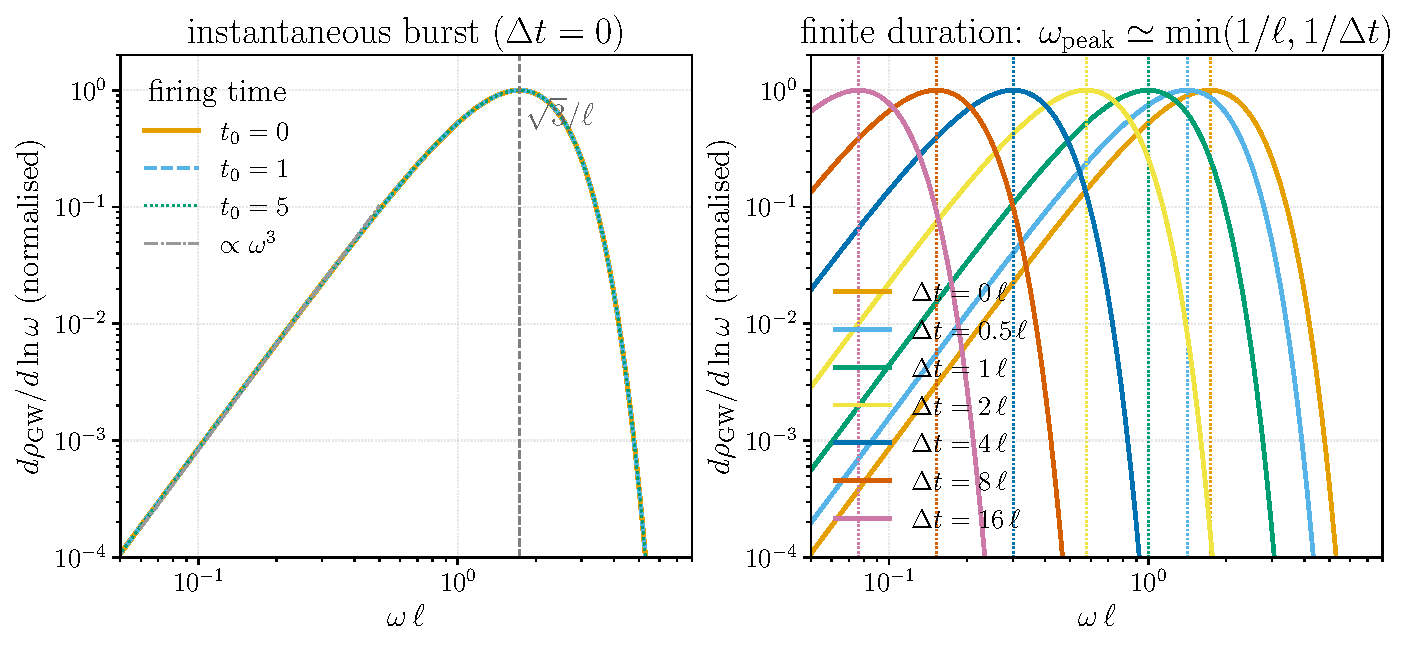
\includegraphics[width=0.92\textwidth]{impulsive_realspace_spectrum}
  \caption{Impulsive-source GW spectrum of Sec.~\ref{sec:impulsive-realspace}.
  \emph{Plotted quantity.} The curves are the GW energy density per logarithmic
  frequency, Eq.~\eqref{eq:rs2-spectrum} with the duration filter
  $|\tilde g(\omega)|^2$ of Eq.~\eqref{eq:rs2-spectrum-dt},
  $d\rho_{\rm GW}/d\ln\omega=8G\,\omega^2\!\int_0^\infty\! dr\,r\sin(\omega r)\,
  \Sigma(r)\,|\tilde g(\omega)|^2$.
  \emph{Source model.} The TT-projected stress two-point function is taken isotropic
  and Gaussian in real space,
  $\Sigma(r)=\langle\mathcal{S}_{ij}(\br_1)\mathcal{S}_{ij}(\br_2)\rangle
  =e^{-r^2/2\ell^2}$ with $|\br_1-\br_2|=r$ and coherence length $\ell$ --- a
  single-scale stand-in for the contracted correlator
  $R_{aa}R_{bb}+\tfrac13R_{ab}R_{ab}$ (the absolute amplitude is irrelevant: every
  curve is normalised to unit peak). Its radial transform
  $P(\omega)=(4\pi/\omega)\!\int_0^\infty\! r\sin(\omega r)\Sigma\,dr
  =(2\pi)^{3/2}\ell^3 e^{-\omega^2\ell^2/2}$ is used in closed form (verified against
  the numerical radial quadrature to $\sim\!10^{-15}$ relative).
  \emph{Temporal profile.} The burst window is Gaussian of width $\Delta t$, giving
  the on-shell temporal filter $|\tilde g(\omega)|^2=e^{-\omega^2\Delta t^2}$;
  $\Delta t=0$ is the instantaneous $\delta(t-t_0)$ limit ($|\tilde g|^2=1$, white in
  source frequency). \emph{Units.} $G=1$, $\ell=1$; the abscissa is $\omega\ell$.
  \emph{Left:} instantaneous burst ($\Delta t=0$) for firing times
  $t_0=0,1,5$ --- the three curves coincide exactly, since $t_0$ enters only as the
  phase $e^{i\omega t_0}$ that cancels in the modulus (Eq.~\eqref{eq:rs2-spectrum});
  the dash--dotted line is the causal $\omega^3$ infrared law and the dashed vertical
  marks the peak $\omega_{\rm peak}=\sqrt{3}/\ell$.
  \emph{Right:} finite duration $\Delta t/\ell=0,0.5,1,2,4,8,16$; dotted verticals are
  the analytic peaks $\omega_{\rm peak}=\sqrt{3}/\sqrt{\ell^2+2\Delta t^2}$, sliding
  from the coherence-limited $\sqrt3/\ell$ (fast burst) to the duration-limited
  $\sqrt{3/2}/\Delta t$ (slow burst), i.e.\ $\omega_{\rm peak}\simeq\min(1/\ell,1/\Delta t)$.
  Generated by \texttt{Notebooks/impulsive\_realspace\_spectrum.py}.}
  \label{fig:impulsive-realspace}
\end{figure*}
\fi

\subsection{Single-scale limit: deriving the quadrupole factor of two}
\label{sec:rs2-monochromatic}

The peak tracks whatever scale the source correlations carry; the cleanest limit is a
fluid coherent at a single length scale $\ell_0$. Here the factor of two relating the
GW scale to the fluid scale is not an assumption --- it follows from the source being
the \emph{quadratic} Reynolds stress $\mathcal{S}_{ij}=w\,v_iv_j$, through Wick's
theorem. For a Gaussian velocity field the connected stress two-point function is
quadratic in the velocity correlator
$R_{ab}(\br)=\langle v_a(\br_1)v_b(\br_2)\rangle$ (the disconnected pairing is the
constant mean stress $\langle\mathcal{S}_{ij}\rangle^2$ and does not radiate):
\begin{equation}
  \Sigma(\br)=\bigl\langle\mathcal{S}_{ij}(\br_1)\mathcal{S}_{ij}(\br_2)\bigr\rangle_{\rm c}
  = w^2\Bigl[R_{aa}(\br)R_{bb}(\br)+\tfrac13 R_{ab}(\br)R_{ab}(\br)\Bigr]
  \;\propto\; R(\br)^2,
  \label{eq:rs2-wick}
\end{equation}
the TT-contracted form of Eq.~\eqref{eq: main}; the key feature is that $\Sigma$ is the
\emph{square} of the velocity correlator. A fluid coherent at the single scale $\ell_0$
has a velocity correlator that oscillates on that scale: for the isotropic single-scale
field the trace is $R_{aa}(r)\propto\sin(r/\ell_0)/(r/\ell_0)$.%
\footnote{This is the standard spectral-tensor result for homogeneous isotropic
turbulence \cite{Batchelor1953,Pope2000,MoninYaglom1975,1959Kraichnan}. Incompressibility
fixes the velocity correlator's tensor structure, leaving its radial part set by a
single scalar; the trace transforms as
$R_{aa}(r)=2\int_0^\infty E(k)\,\frac{\sin kr}{kr}\,dk$ with $E$ the energy spectrum, so
a fluid carrying a single scale ($E$ concentrated at one $1/\ell_0$) gives
$R_{aa}(r)\propto\sin(r/\ell_0)/(r/\ell_0)$ and $R_{aa}(0)=\langle v^2\rangle$.
Physically $\sin(r/\ell_0)/(r/\ell_0)$ is the directional average of a plane wave over
the sphere of fixed scale --- the correlation of a random field built from equal-size
eddies pointing every way: it first vanishes at $r=\pi\ell_0$ (points half a wavelength
apart are anti-correlated) and decays as $\ell_0/r$ as the phases wash out. The same
angular reduction underlies the GW-from-turbulence kernels
\cite{2002Kosowsky,2007Gogoberidze}.}
Squaring \emph{halves the scale},
\begin{equation}
  R(r)^2\;\propto\;\frac{\sin^2(r/\ell_0)}{(r/\ell_0)^2}
  =\frac{1-\cos(2r/\ell_0)}{2\,(r/\ell_0)^2},
  \label{eq:rs2-square}
\end{equation}
so the radiating part of $\Sigma(r)$ oscillates on the halved scale $\ell_0/2$ (the
constant term is the non-radiating mean). The GW frequency is the inverse of the scale
it samples, so the spectrum
$d\rho_{\rm GW}/d\ln\omega\propto\omega^3 P(\omega)|\tilde g(\omega)|^2$ collapses to a
single line at
\begin{equation}
  \boxed{\;
  \omega_{\rm GW}=\frac{2}{\ell_0}
  \qquad\bigl(\ell_{\rm GW}=\tfrac12\,\ell_0\bigr).\;}
  \label{eq:rs2-mono-peak}
\end{equation}
The factor of two is thus \emph{derived}: a quadratic (quadrupole) source $v_iv_j$
radiates on half the scale --- twice the frequency --- of the field that drives it,
Eq.~\eqref{eq:rs2-square} being that halving written as the identity
$\sin^2\theta=\tfrac12(1-\cos2\theta)$. There is no infrared $\omega^3$ rise and no
ultraviolet falloff: the $\omega^3$ phase space and the duration filter
$|\tilde g(\omega)|^2$ fix only the line's height, so $\omega_{\rm GW}$ is independent
of both the firing time $t_0$ and the duration $\Delta t$. This is the
configuration-space image of the GW peak at half the source scale found for the
monochromatic source in Eq.~\eqref{eq:impulsive-peak}: two velocity features of scale
$\ell_0$ overlap to produce stress structure on the scale $\ell_0/2$.
(A strictly single-scale field in
fact fills all scales $\ge\ell_0/2$ --- the autoconvolution in Eq.~\eqref{eq:rs2-wick}
--- piling up at the $\ell_0/2$ edge as in Sec.~\ref{sec:impulsive}; the $\delta$-line
keeps only the halved scale.)

\iffalse  % proof-of-concept figure (commented out)
\begin{figure*}[ht]
  \centering
  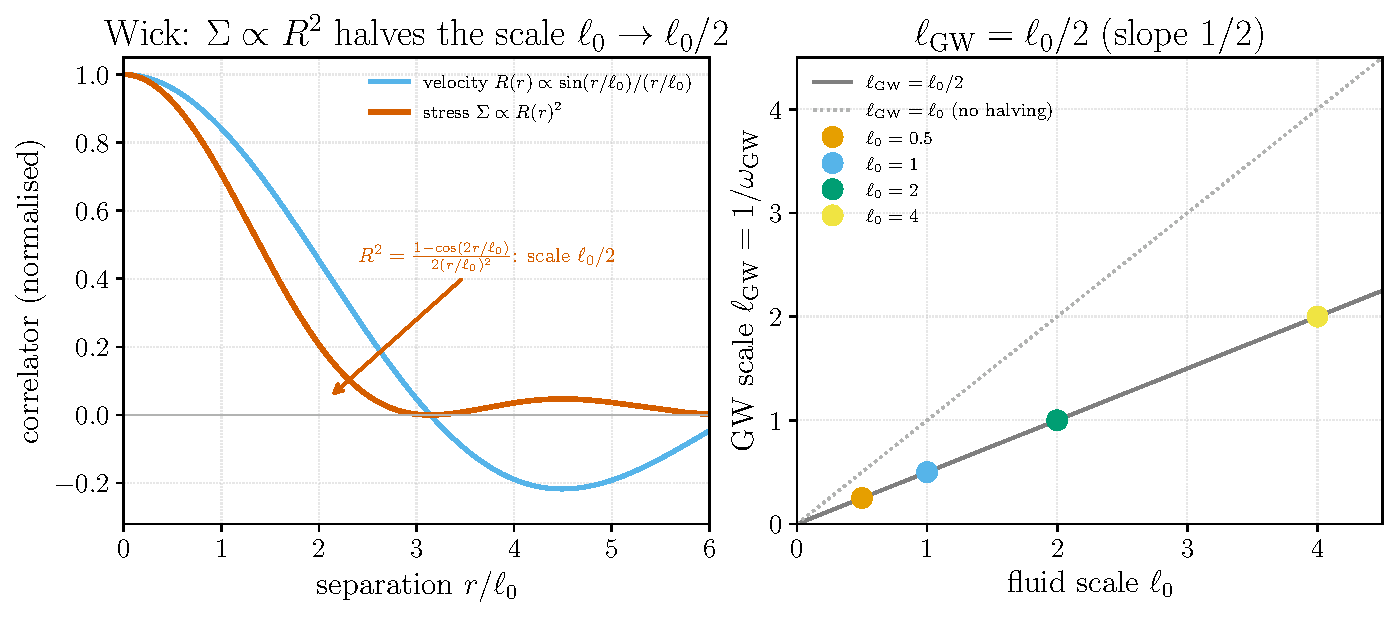
\includegraphics[width=0.92\textwidth]{impulsive_monochromatic_source}
  \caption{Single-scale toy of Sec.~\ref{sec:rs2-monochromatic}: the quadrupole factor
  of two, derived in the length-scale picture. \emph{Left:} the derivation itself
  (Eqs.~\eqref{eq:rs2-wick}--\eqref{eq:rs2-square}). A fluid coherent at one scale
  $\ell_0$ has the velocity correlator $R(r)\propto\sin(r/\ell_0)/(r/\ell_0)$ (blue);
  because the GW source is the quadratic Reynolds stress $\mathcal{S}_{ij}\sim v_iv_j$,
  the radiating stress correlator is its square $\Sigma\propto R(r)^2$ (orange), which
  by $\sin^2=\tfrac12(1-\cos2\,\cdot)$ oscillates on the \emph{halved} scale
  $\ell_0/2$. \emph{Right:} the resulting GW scale is exactly half the fluid scale,
  $\ell_{\rm GW}=\ell_0/2$ (solid, slope $1/2$; points $\ell_0=0.5,1,2,4$), versus the
  unhalved $\ell_{\rm GW}=\ell_0$ (dotted) --- equivalently $\omega_{\rm GW}=2/\ell_0$
  (Eq.~\eqref{eq:rs2-mono-peak}). The line carries no causal $\omega^3$ rise and no
  ultraviolet decay, and its position is independent of the firing time $t_0$ and
  duration $\Delta t$. Generated by
  \texttt{Notebooks/impulsive\_monochromatic\_source.py}.}
  \label{fig:impulsive-monochromatic}
\end{figure*}
\fi

\section{\texorpdfstring{Numerical results: $f_{\rm peak}^{\rm GW}(\tau_\ast, M_0)$}{Numerical results: f\_peak\^GW(tau, M0)}}
\label{sec:fpeak-numerical}

We scan the peak GW frequency
$f_{\rm peak}^{\rm GW}=\operatorname{argmax}_\omega[\omega\,\Omega_{\rm GW}(\omega)]/2\pi$
over the $(\tau_\ast,M_0)$ plane for a delta-shell decaying source evolved with
the BK2016 self-similar closure and time-integrated over the emission window
(\texttt{Notebooks/f\_peak\_vs\_tau\_mach.py}). Two temporal-correlation kernels
are compared through their dimensionless transform
$\mathcal{G}(q)=\widehat{R^2}(q)$: the random-phase BK2016 form (Model A) and the
coherent eddy (Model B).

Across all four self-similar classes the ratio
$f_{\rm peak}^{A}/f_{\rm peak}^{B}$ is \emph{independent of} $(\tau_\ast,M_0)$:
the self-similar closure makes both the eddy frequency $\omega_e$ and the
sweeping rate $\eta_0$ scale as $(1+T/\tau_\ast)^{-1}$, so the two kernels inherit
the same overall frequency scaling and differ only in their fixed dimensionless
peak position. The model difference therefore collapses to a single per-class
constant (Fig.~\ref{fig:f_peak_model_ratio}): $f_A/f_B\simeq0.37,\,0.36$ for the
HD (Loitsiansky, Saffman) classes and $0.83,\,0.78$ for the MHD (nonhelical,
helical) classes -- Model A always peaks lower. The large HD offset comes from
the side-peak of the coherent kernel at the eddy frequency ($q\simeq\pm2$, the
$\cos\sigma$ oscillation of $R_B$), which wins the $\omega\,\Omega_{\rm GW}$
argmax for the steep-decay HD classes but nearly coincides with the broad
Model-A peak for MHD. Because the per-model maps differ only by this constant, we
display the ratio rather than the eight individual heatmaps.

\begin{figure*}[ht]
  \centering
  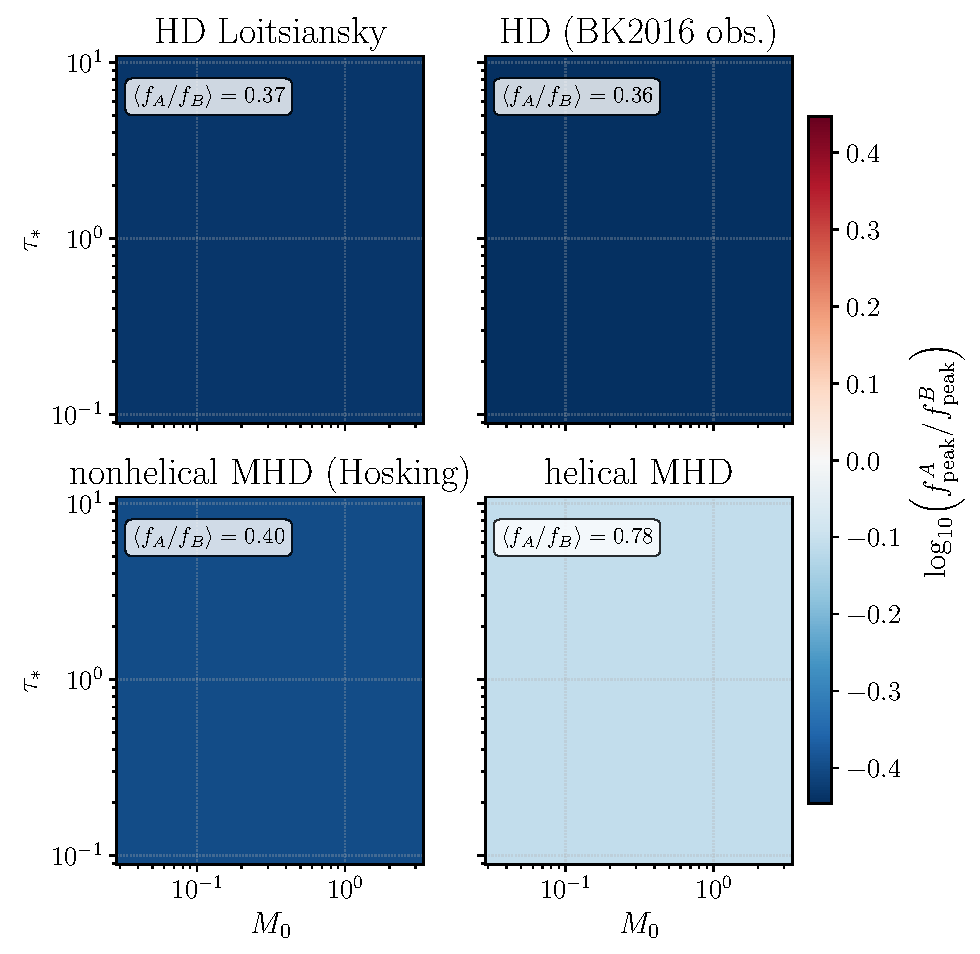
\includegraphics[width=\textwidth]{f_peak_model_difference}
  \caption{Model A/B ratio of the peak GW frequency,
  $\log_{10}(f_{\rm peak}^{A}/f_{\rm peak}^{B})$, on the $(\tau_\ast,M_0)$ plane
  for the four BK2016 self-similar decay classes (HD Loitsiansky $q=2/7$,
  $\beta=4$; HD Saffman $q=1/3$, $\beta=3$; nonhelical MHD $q=1/2$, $\beta=1$;
  helical MHD $q=2/3$, $\beta=0$). Each panel is flat: the ratio is independent
  of $(\tau_\ast,M_0)$, fixed only by the kernel shapes, with the per-class value
  $\langle f_A/f_B\rangle$ annotated. Model A (random-phase) peaks below Model B
  (coherent eddy) everywhere; the HD classes show the larger offset.}
  \label{fig:f_peak_model_ratio}
\end{figure*}


\section{Differences among the models}
\label{sec:model-differences}

With every kernel of Table~\ref{tab:model-grid} in hand we can now say precisely
what distinguishes them, and---more usefully---which of the two axes of
Sec.~\ref{sec:model-space} each difference belongs to. The summary is
Table~\ref{tab:model-differences}; the reasoning follows. Throughout,
$\Omega_{\rm GW}(p)\propto p^{3}H[S,T](p,p)$ and all numbers are measured by
\texttt{Notebooks/model\_grid\_survey.py} at $M=1$, $R=10^{4}$.

\paragraph{The infrared belongs to the spatial axis alone.}
Every kernel with a spatially extended source gives the causal $k^{3}$, and
every kernel with a monochromatic source gives $k^{2}$, \emph{irrespective of
the temporal model}: we measure $3.00$ for $H[S_{\rm K41},T_{\rm sw}]$ and
$2.97$ for $H[S_{\rm K41},T_{\rm dec}]$, against $2.00$ and $1.97$ for the two
$\delta k$ kernels and $2.00$ for the impulsive one. This is not a coincidence
of our kernels but the universal theorem of Sec.~\ref{sec:cps-reproduction}: the
infrared is fixed by whether the source spectrum has finite width, and a
$\delta$-function source violates that hypothesis by exactly one power through
the $1/p$ pole of $\mathcal{K}_{0}(p)/p$. The temporal factor cannot contribute,
because as $p\to0$ it tends to a constant---$\pi\,\mathcal{C}(0)=6\pi$ for
$T_{\rm dec}$ by Eq.~\eqref{eq:cosT-limits}, unity for $T_{\rm sw}$---and a
constant carries no slope. \emph{Corollary:} no choice of UETC can be tuned to
reproduce the simulated $k^{1}$ of Sec.~\ref{sec:principal-discrepancy}. That
tension is not resolvable on the temporal axis, which is precisely why it
survives every treatment in Table~\ref{tab:three-works}.

\paragraph{The ultraviolet belongs to the temporal axis alone.}
Here the roles reverse, and the discriminant is sharp: it is whether the UETC
has a \emph{cusp} at zero lag. By Eq.~\eqref{eq:cusp-tail} the temporal factor
falls as $-2f'(0^{+})/\omega^{2}$, so
\begin{itemize}\itemsep0pt
  \item $T_{\rm sw}$ (Gaussian, $f'(0^{+})=0$): no cusp, and the cutoff is
    super-exponential. Fitting a power law to it is meaningless---the apparent
    ``slope'' merely records where the fit window was placed, which is why
    $H[S_{\delta r},T_{\rm sw}]$ returns $-46.6$ and
    $H[S_{\rm K41},T_{\rm sw}]$ returns $-4.75$ on the same window.
  \item $T_{\rm dec}$ (power law, $f'(0^{+})=-4/3$): a genuine heavy tail
    $\propto\omega^{-2}$, with the coefficient $8/3$ of
    Eq.~\eqref{eq:cosT-limits}. The measured GW slope is mildly $M$-dependent
    ($-1.65$ at $M=0.05$ rising to $-1.28$ at the formal $M=3$) because the tail
    sets in only above $q\sim M$.
  \item $T_{\rm imp}$, $T_{\rm burst}$: white and window-modulated respectively,
    the latter carrying the $\sin^{2}$ factor of Eq.~\eqref{eq:window-factor}.
\end{itemize}
This single dichotomy---cusp or no cusp---is what the caveat of
Sec.~\ref{sec:decaying-peak} turns on, and it is worth emphasising that it is
\emph{not} a matter of degree: the two behaviours differ by fourteen orders of
magnitude by $q=4$.

\paragraph{The peak is where the two axes compete.}
The peak is the one property neither axis owns outright, which is why it has
been the most contested quantity in the literature. With $T_{\rm sw}$ the
spectrum is cut off at the sweeping frequency and the peak sits at
$p\simeq1.47M$ (measured $1.53$ at $M=1$), \emph{below} the source scale for
subsonic turbulence. With $T_{\rm dec}$ the heavy tail survives past that
cutoff, and the peak is instead pinned by the spatial structure at
$p\simeq2.3$, essentially independent of $M$ (measured $2.32$ for
$M\le1$, drifting to $2.79$ by the formal $M=3$). The two temporal models therefore
disagree about the peak by a factor $\sim1/M$, which for the subsonic
simulations is an order of magnitude---this is exactly the
Gogoberidze-versus-Roper~Pol tension of Sec.~\ref{sec:peak-location}. Note that
the $\delta k$ and $\delta r$ kernels have no dynamical peak at all: the former
is truncated at $p=2$ by the triangle inequality, and the latter, having
$E\propto k^{2}$, is ultraviolet-dominated and simply rises to the dissipation
cutoff. Their tabulated ``peaks'' are cutoffs, not physics.

\paragraph{Positivity is a property of the temporal axis, and not automatic.}
The temporal factor must be non-negative at every frequency, since it is the
power spectrum of a real correlation; a UETC that fails this yields negative
gravitational-wave energy. This is not a hypothetical failure mode---it is the
defect that led Caprini et al.\ to discard a Gaussian straining-time model in
favour of a top-hat, and that motivates the positive-definite Gibbs kernel of
\cite{2022Auclair}. Both temporal models used here are safe, and for
$T_{\rm dec}$ provably so: $(1+s)^{-4/3}$ is completely monotone, hence by
Bernstein's theorem a superposition of decaying exponentials, whose cosine
transforms $2a/(a^{2}+\omega^{2})$ are individually positive; products of
completely monotone functions are completely monotone, so the two-scale factor
Eq.~\eqref{eq:two-scale-feynman} inherits the property. We verify
$\mathcal{C}>0$ over $10^{-8}<q<10^{4}$.

\subsection{The Mach exponent of the peak as a regime diagnostic}
\label{sec:mach-exponent}

The peak's dependence on the Mach number deserves separating out, because it is
the one place where the two temporal models make a \emph{qualitatively}
different prediction rather than a quantitatively different one. Measuring
$d\ln p_{\rm peak}/d\ln M$ at fixed $k_0$ over $M\in[0.1,1.6]$ (the upper end
formal, $M>1$ being superluminal, but included to pin the exponent) gives
\begin{center}
\begin{tabular}{lc}
\hline
Temporal model & $d\ln p_{\rm peak}/d\ln M$ \\
\hline
$T_{\rm sw}$ (Kraichnan sweeping) & $+0.974$ \\
$T_{\rm dec}$ (BK2016 power law)  & $+0.048$ \\
$T_{\rm imp}$ ($\delta$-in-time)  & $\phantom{+}0.000$ \\
\hline
\end{tabular}
\end{center}
a clean split between unity and zero. The mechanism is transparent: $T_{\rm sw}$
multiplies the spectrum by $e^{-q^{2}/M^{2}}$, a cutoff at $q\sim M$, so the peak
simply tracks that cutoff; $T_{\rm dec}$ and $T_{\rm imp}$ impose no such
frequency scale, so the peak falls back on the spatial structure. Strikingly,
the integrated energy is nearly \emph{blind} to this distinction---we measure
$E_{\rm tot}\propto M^{5.8}$ and $M^{5.6}$ for the two---so it is the peak, not
the amplitude, that carries the information.

\paragraph{What is and is not new here.} Both halves of this contrast are
already in the literature, and neither is ours. Gogoberidze et al.\
\cite{2007Gogoberidze} state that the peak frequency scales linearly with the
characteristic velocity, i.e.\ $f_{\rm peak}\propto Mk_{0}$---our stationary row,
of which the coefficient $1.47$ of Sec.~\ref{sec:peak-location} is a
quantitative refinement. Auclair et al.\ \cite{2022Auclair} find instead that the
peak is pinned to the integral scale independently of the velocity---our
decaying and impulsive rows. What appears not to have been said is that the two
sit on a single axis and that the exponent itself is therefore a diagnostic:
\cite{2022Auclair} in particular does not contrast the velocity dependence
between decorrelating and coherent sources.

\paragraph{What the diagnostic actually diagnoses.} It is tempting to read the
table as evidence for the power-law UETC specifically, and that reading is
wrong. The impulsive kernel contains no $M$ anywhere, so its exponent is
identically zero while having no heavy tail, no power law, and indeed no
temporal structure at all; and \cite{2022Auclair} obtain a velocity-independent
peak while using Kraichnan \emph{sweeping}, because in a freely decaying flow the
integral scale itself evolves. Velocity-independence of the peak is therefore a
property of a whole class of sources, not a signature of
Eq.~\eqref{eq:cosT-closed}. The exponent answers ``does the temporal factor
impose a cutoff at $q\sim M$?''---not ``which UETC is it?''. Read that way it is
a genuine diagnostic; read as support for the decaying model in particular it
proves much less than it appears to, and the peak-based argument of
Sec.~\ref{sec:decaying-peak} should be weighted accordingly.

\paragraph{The aeroacoustic precedent.} That the Mach scaling is regime-dependent
is classical, and the relevant distinction is precisely a temporal one.
Lighthill's eighth-power law \cite{Lighthill1952} ($P\propto U^{8}$, fixed
velocity and geometry) and Proudman's \cite{Proudman1952}
($P\propto\rho\varepsilon M^{5}$, isotropic turbulence at fixed dissipation
rate) differ in what is held fixed---the same ambiguity that flips our own peak
scaling between $1.47M$ at fixed $k_{0}$ and $1.47/M^{2}$ at fixed $\varepsilon$.
More pointedly, Proudman's $M^{5}$ rests on \emph{neglecting retarded-time
differences}, replacing the retarded covariance of the stress by the simultaneous
one---that is, on treating the source as temporally coherent---and Lilley
\cite{Lilley1994} later rederived the result retaining them. The coherent versus
decorrelating axis that separates our two rows is thus the Proudman--Lilley
question transposed into a cosmological setting, and our integrated
$M^{5.6}$--$M^{5.8}$ sits near Proudman's $M^{5}$. The contribution here is not
the existence of a regime dependence but its sharpening into a spectral
observable: an exponent one reads off the peak rather than off the total power.
(The two integrated exponents are approximate; the stationary kernel emits
convergence warnings over this sweep.)

\paragraph{Analytic structure.} Finally, the models differ in what must actually
be computed, and the reduction is larger than the usual presentation suggests.
The decaying kernels are conventionally written as frequency convolutions of the
singular $\hat g$, which is both expensive and numerically treacherous; by
Eqs.~\eqref{eq:conv-equals-cosT} and \eqref{eq:two-scale-feynman} the
single-scale case is closed-form and the two-scale case is a single smooth
Gauss--Jacobi quadrature over the closed form. The decaying kernels are
therefore no harder than the Gaussian ones.

\begin{table*}[ht]
  \centering
  \begin{tabular}{lccccl}
  \hline
  Kernel & IR slope & Peak $p$ & UV & Positive & Literature counterpart \\
  \hline
  $H[S_{\rm K41},T_{\rm sw}]$   & $3.00$ & $1.47M$ & super-exp & yes & Gogoberidze et al.~\cite{2007Gogoberidze} \\
  $H[S_{\rm K41},T_{\rm dec}]$  & $2.97$ & $2.32$ & $\omega^{-2}$ & yes & Roper Pol et al.~\cite{2019RoperPol} (peak) \\
  $H[S_{\delta k},T_{\rm sw}]$  & $2.00$ & cutoff & none & yes & --- \\
  $H[S_{\delta k},T_{\rm dec}]$ & $1.97$ & cutoff & none & yes & --- \\
  $H[S_{\delta r},T_{\rm sw}]$  & $3.00$ & cutoff & super-exp & yes & --- \\
  $H[S_{\delta r},T_{\rm dec}]$ & $2.97$ & cutoff & $\omega^{-2}$ & yes & --- \\
  $H[S_{\delta k},T_{\rm imp}]$ & $2.00$ & cutoff & none & yes & --- \\
  \hline
  \end{tabular}
  \caption{Systematic comparison of the kernels of Table~\ref{tab:model-grid},
  measured at $M=1$, $R=10^{4}$ on the diagonal $q=p$ by
  \texttt{Notebooks/model\_grid\_survey.py}. The infrared slope tracks the
  \emph{spatial} axis only ($3$ for extended sources, $2$ for monochromatic
  ones, per Sec.~\ref{sec:cps-reproduction}); the ultraviolet tracks the
  \emph{temporal} axis only (a power-law tail iff the UETC has a cusp at zero
  lag, Eq.~\eqref{eq:cusp-tail}); only the peak depends on both. ``cutoff''
  denotes models with no dynamical peak---the $\delta k$ kernels are truncated
  at $p=2$ by the triangle inequality and the $\delta r$ kernels are
  ultraviolet-dominated. ``super-exp'' denotes a Gaussian cutoff, for which no
  power-law slope exists.}
  \label{tab:model-differences}
\end{table*}

\section{Spectrum survey for all derived models}
\label{sec:spectrum-survey}

In this section we plot, on a common convention, the dimensionless GW
energy-density spectrum
\begin{equation}
  \Omega_{\rm GW}(p) \;\propto\; p^{3}\,H(p,p),
  \qquad p = k_{\rm GW}/k_0,
\end{equation}
along the sound-cone diagonal $q = p$ for every model derived in this paper,
in the uniform notation $H[S,T]$ of Sec.~\ref{sec:model-space}. The $p^{2}$
factor relative to the characteristic strain $h_c^{2}(p) = p\,H(p,p)$ is the
phase-space measure $d^{3}k$; together with causality and a source of finite
spectral width it predicts $\Omega_{\rm GW}\sim p^{3}$ in the IR, followed by a
peak and a decay in the UV. A dotted grey line shows the $p^{3}$ reference.

These plots are the graphical form of Table~\ref{tab:model-differences}, and
should be read with its two organising facts in mind: the infrared slope is
fixed by the \emph{spatial} model alone and the ultraviolet by the
\emph{temporal} model alone. In particular the monochromatic panels sit at
$p^{2}$ rather than $p^{3}$ not because of anything in their temporal treatment
but because a zero-width source carries a $1/p$ pole,
$\mathcal{K}_{0}(p)/p$, which is exactly the $\delta$-function exception to the
universal infrared theorem reproduced in Sec.~\ref{sec:cps-reproduction}. The
build log of \texttt{Notebooks/all\_spectra.py} flags cases whose IR slope
departs from $3$ by more than $\pm0.5$; the monochromatic models are expected
to be flagged, and are not anomalies.

\begin{figure}[ht]
  \centering
  \begin{minipage}{0.48\columnwidth}
    \centering
    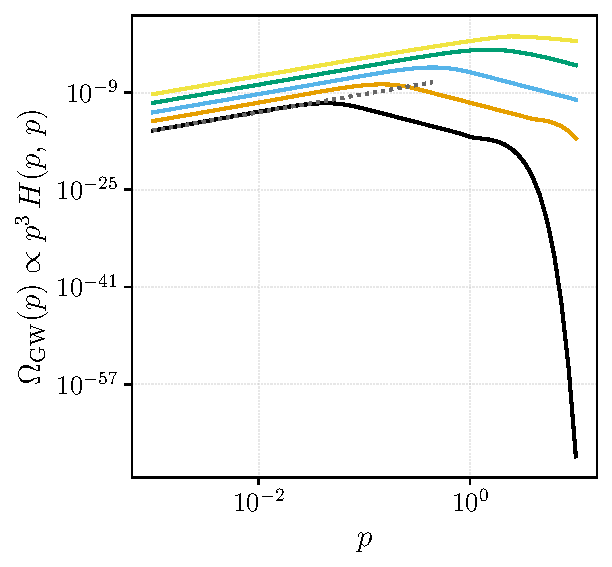
\includegraphics[width=\textwidth]{spectrum_kraichnan_kolmogorov}\\
    \textit{(a) full $H_{pq}$}
  \end{minipage}\hfill
  \begin{minipage}{0.48\columnwidth}
    \centering
    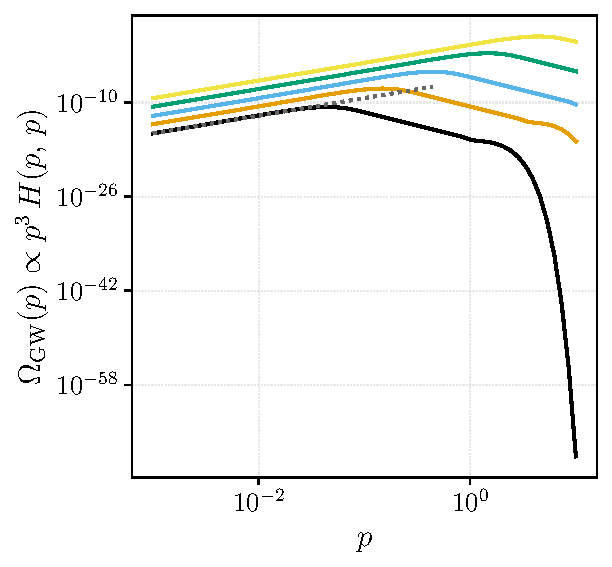
\includegraphics[width=\textwidth]{spectrum_aeroacoustic_limit}\\
    \textit{(b) $p\to 0$ limit}
  \end{minipage}
  \caption{Kraichnan decorrelation + Kolmogorov spectrum.  Five curves per
  panel correspond to $M = 0.03,\, 0.1,\, 0.3,\, 1.0,\, 3.0$ at $R=10^{4}$.
  Panel (a) is the full numerical $H_{pq}$ (Sec.~\ref{sec:kraichnan-k41}); panel (b) is the
  aeroacoustic $p\to 0$ limit (Kahniashvili et al.\ 2008).  Both give the
  universal IR slope $\Omega_{\rm GW}\propto p^{3}$.}
  \label{fig:spectrum_kolmogorov_kraichnan_pair}
\end{figure}

\begin{figure}[ht]
  \centering
  \begin{minipage}{0.48\columnwidth}
    \centering
    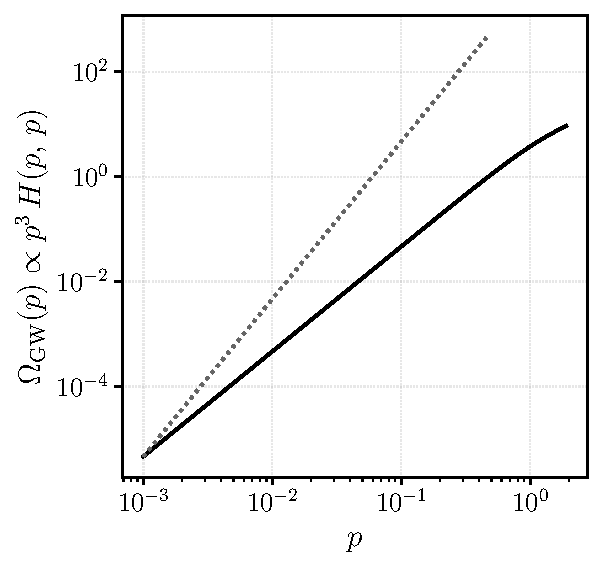
\includegraphics[width=\textwidth]{spectrum_delta_k_kraichnan}\\
    \textit{(a) Kraichnan}
  \end{minipage}\hfill
  \begin{minipage}{0.48\columnwidth}
    \centering
    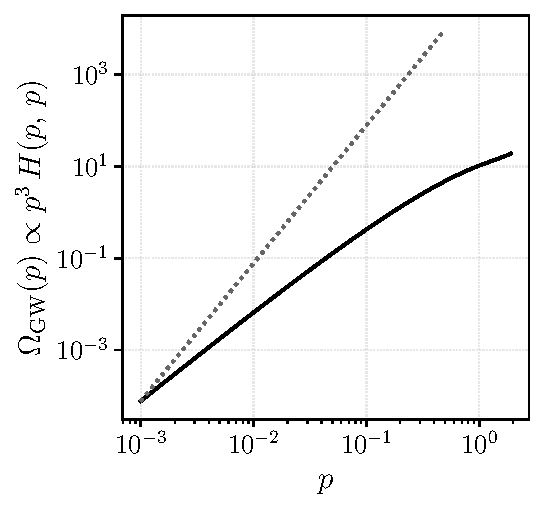
\includegraphics[width=\textwidth]{spectrum_delta_k_decay}\\
    \textit{(b) Decay}
  \end{minipage}
  \caption{Monochromatic spectrum $E(k)=E_{0}\delta(k-k_{0})$ (no free
  parameters at the dimensionless level).  Panel (a): Kraichnan
  decorrelation, closed form $\Omega_{\rm GW}(p)\propto
  p^{3}\,K_{0}(p)/p\,\Theta(2-p)\,e^{-p^{2}/(2\pi)}$ with IR slope
  $\mathbf{2}$ (flagged: $1/p$ pole from the monochromatic source removes
  one power of $p$ from the universal scaling).  Panel (b): decay temporal
  factor, Eq.~\eqref{eq:conv-equals-cosT}, IR slope $\mathbf{2}$ --- the
  \emph{same} slope as panel (a), as it must be, since the temporal factor
  tends to the constant $\pi\,\mathcal{C}(0)$ as $p\to0$ and so cannot alter
  the infrared scaling.}
  \label{fig:spectrum_delta_k_pair}
\end{figure}

\begin{figure}[ht]
  \centering
  \begin{minipage}{0.48\columnwidth}
    \centering
    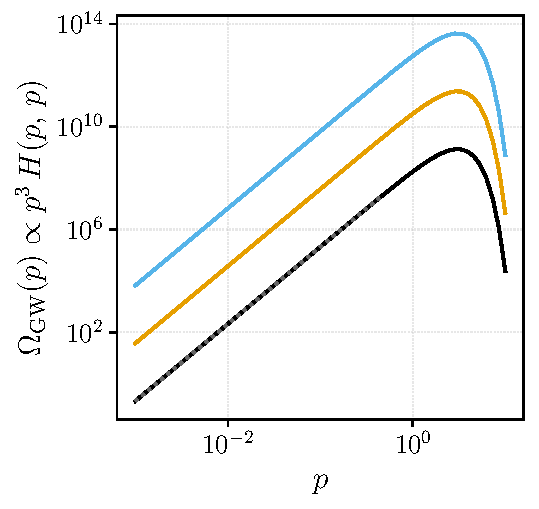
\includegraphics[width=\textwidth]{spectrum_white_kraichnan}\\
    \textit{(a) Kraichnan}
  \end{minipage}\hfill
  \begin{minipage}{0.48\columnwidth}
    \centering
    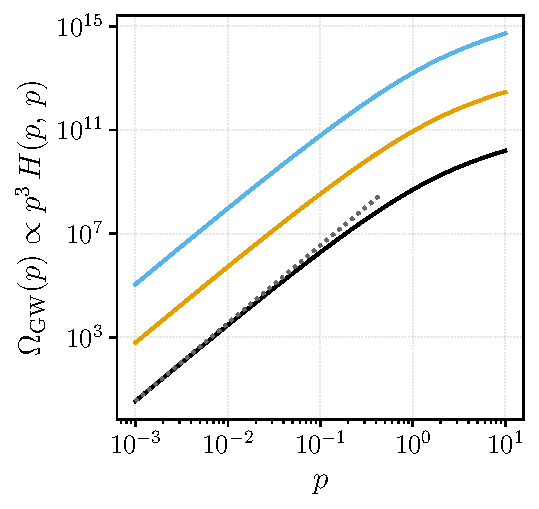
\includegraphics[width=\textwidth]{spectrum_white_decay}\\
    \textit{(b) Decay}
  \end{minipage}
  \caption{White-noise real-space correlations
  $R_{ij}\propto\delta^{(3)}(\br)$.  Three curves per panel correspond to
  $R = 10^{3},\, 10^{4},\, 10^{5}$.  Panel (a): Kraichnan decorrelation,
  matches the universal IR slope $\mathbf{3}$.  Panel (b): decay temporal
  model, IR slope $\mathbf{3}$ as well, for all three $R$ --- the decaying
  and Kraichnan models share the universal causal infrared, the temporal
  factor affecting only the amplitude and the ultraviolet tail.}
  \label{fig:spectrum_white_pair}
\end{figure}


\subsection{All nine kernels side by side}
\label{sec:kernel-grid}

Figure~\ref{fig:kernel_comparison_grid} places every entry of
Table~\ref{tab:model-grid} on one figure, at matched parameters, with the
abscissa in units of the initial-power peak $k_0$ throughout. The comparison is
organised by a single control common to all nine panels, the source coherence
time in units of the light-crossing time of the source scale,
\begin{equation}
  \hat\tau \;\equiv\; \tau_c\,k_0 ,
  \qquad
  \omega\tau_c\big|_{\omega=k}=p\,\hat\tau ,
  \label{eq:that}
\end{equation}
so that the dimensionless temporal argument of every kernel is the same
function $p\hat\tau$ of the plotted abscissa. For the sweeping models
$\tau_c=\tau_{k_0}=\sqrt{2\pi}/(Mk_0)$, i.e.\ $M=\sqrt{2\pi}/\hat\tau$; for the
finite burst $\tau_c=\Delta t$, giving the low-pass $|\tilde
g|^2=e^{-p^2\hat\tau^2}$ of Eq.~\eqref{eq:rs2-spectrum-dt}. The stationary and
time-independent kernels ($T_{\rm sw}$, $T_{\rm imp}$) carry a single line at
$\hat\tau=1$; the time-dependent ones ($T_{\rm dec}$, $T_{\rm burst}$) are shown
at $\hat\tau=0.01,0.1,1,10,100$.

Three things are visible at a glance, and each is the graphical form of a
statement made analytically above.

\emph{The infrared is set by the spatial model alone.} Every $S_{\rm K41}$,
$S_{\rm full}$ and $S_{\delta r}$ panel sits on $p^{3}$ ($2.91$--$3.00$
measured) regardless of which temporal model multiplies it and regardless of
$\hat\tau$, while every $S_{\delta k}$ panel sits on $p^{2}$ ($1.91$--$2.00$).
The one power of difference is the $1/p$ pole of $\mathcal{K}_0(p)/p$ carried by
a zero-width source, the $\delta$-function exception to the universal infrared
theorem of Sec.~\ref{sec:cps-reproduction}. Changing $\hat\tau$ by four decades
moves the infrared amplitude but never its slope, which is
Eq.~\eqref{AR:IR} restated: as $p\to0$ the temporal factor tends to a constant
[$\mathcal{C}(0)=6$, Eq.~\eqref{A:Climits}] and cannot alter the infrared
scaling.

\emph{The ultraviolet is set by the temporal model alone.} Only the three
$T_{\rm dec}$ panels have a power-law tail, inherited from the
$\bar q^{-2}$ cusp tail of Eq.~\eqref{eq:cosT-limits}; the sweeping and burst
kernels cut off as Gaussians, for which a fitted log-log slope is a property of
the fitting window and not of the model, and is therefore reported as
``Gaussian'' rather than as a number. The monochromatic panels terminate
at $p=2$ on the triangle inequality $\Theta(2-p)$ instead.

\emph{The peak responds to both, and in opposite ways.} At $\hat\tau=1$ the
peaks cluster at $p_{\rm pk}=2.0$--$3.2$, i.e.\ at the source scale. Lengthening
the coherence time drives them apart: the $T_{\rm burst}$ peak slides down as
$p_{\rm pk}\simeq1/\hat\tau$, the duration-limited branch of
Eq.~\eqref{eq:rs2-fpeak-dt}, whereas the $T_{\rm dec}$ peaks stay pinned near
the source scale because the heavy $\bar q^{-2}$ tail keeps supplying power at
$\omega=k$ (Sec.~\ref{sec:decaying-peak}). $H[S_{\delta r},T_{\rm dec}]$ has no
peak at all in the plotted range: a white spatial source is ultraviolet
dominated by construction ($E\propto k^{2}$) and its maximum is set by the
dissipation cutoff $R^{3/4}$, not by any dynamical scale, which is why the
panel is labelled UV-limited rather than assigned a peak.

\begin{figure}[ht]
  \centering
  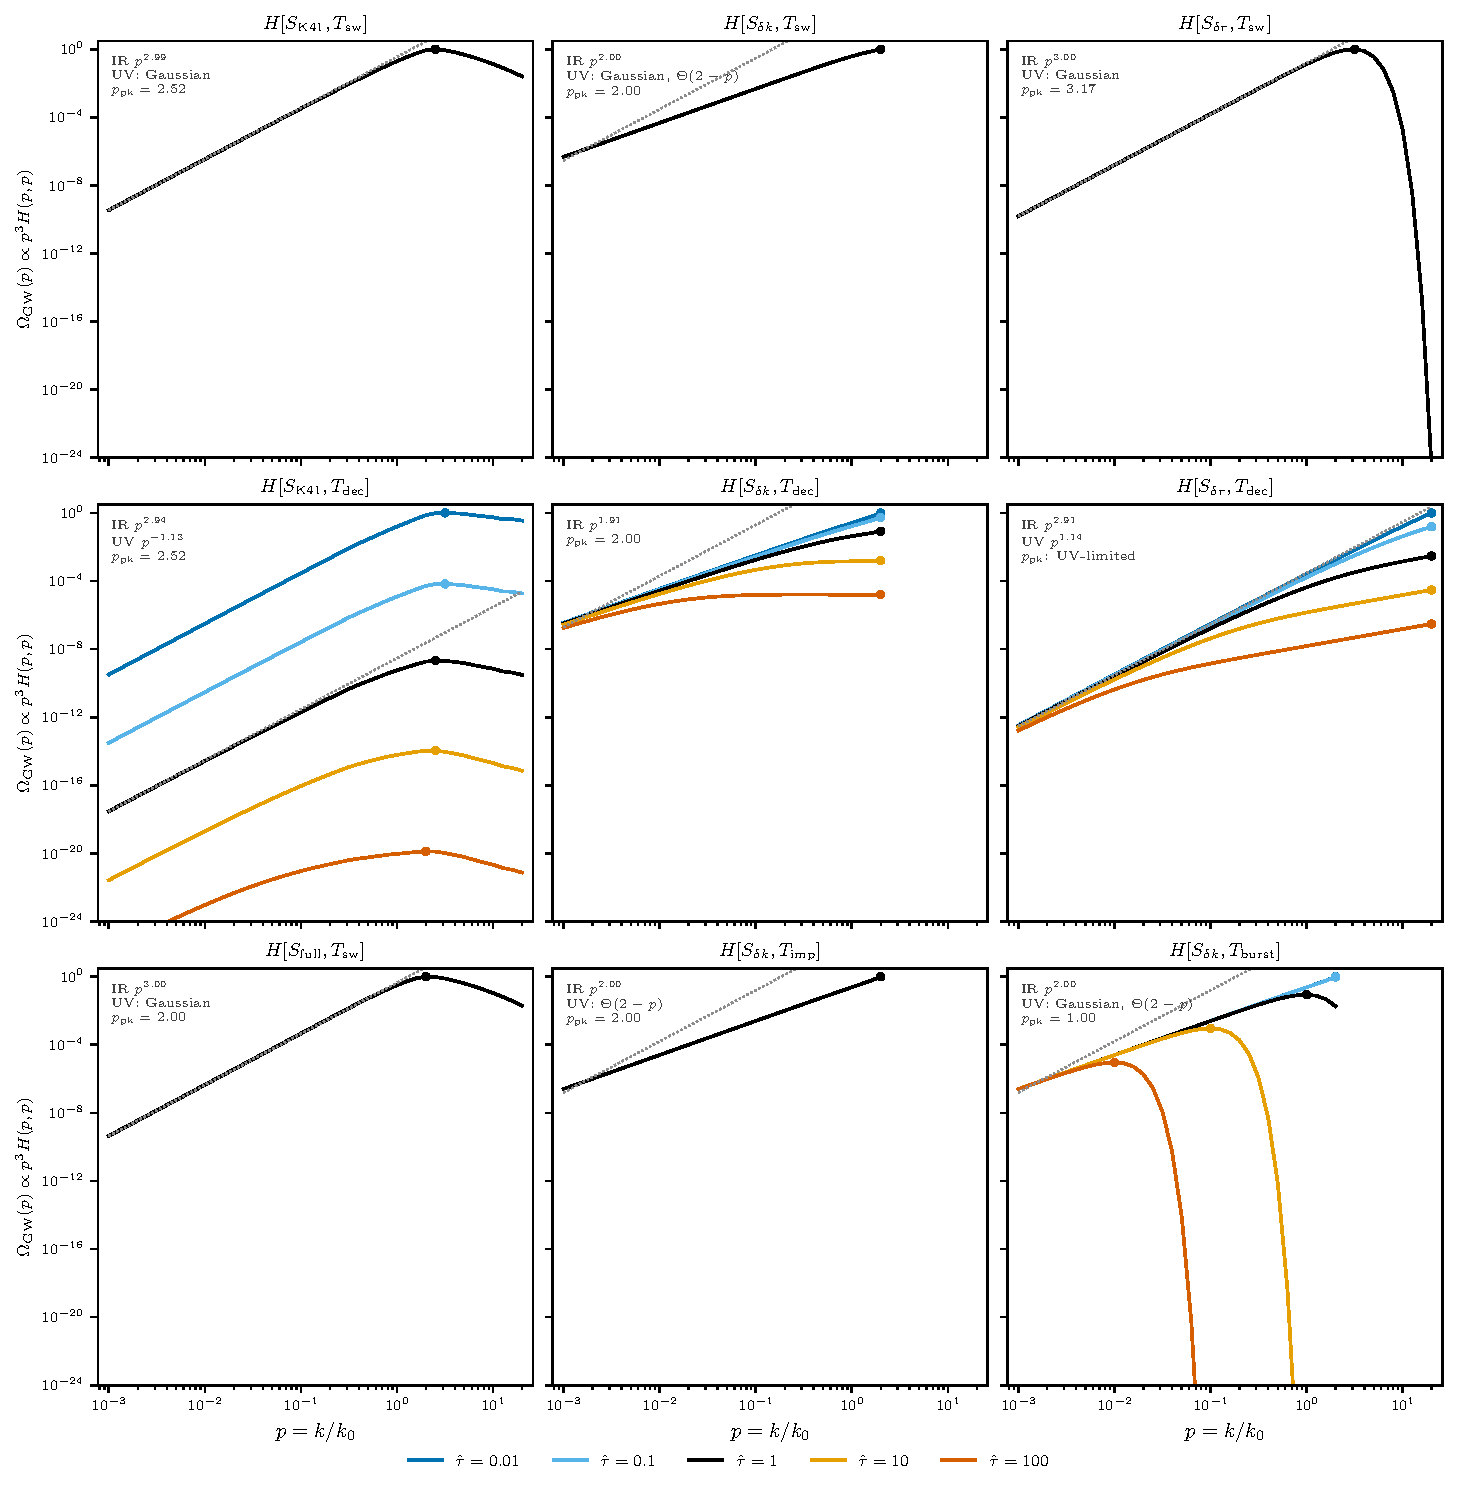
\includegraphics[width=\columnwidth]{kernel_comparison_grid}
  \caption{The nine kernels of Table~\ref{tab:model-grid} at matched
  parameters, $\Omega_{\rm GW}(p)\propto p^{3}H[S,T](p,p)$ on the sound-cone
  diagonal, $p=k/k_0$, at $R=10^{4}$ (and $R_{\rm IR}=10^{2}$ with a Batchelor
  infrared band for $S_{\rm full}$). Rows group the temporal model: sweeping
  (top), decaying (middle), and the full-spectrum, impulsive and burst cases
  (bottom). Curves are indexed by $\hat\tau=\tau_ck_0$ of Eq.~\eqref{eq:that};
  stationary and time-independent kernels carry the single reference line
  $\hat\tau=1$ (equivalently $M=\sqrt{2\pi}=2.51$ for the sweeping panels), the
  time-dependent ones the five values $\hat\tau=0.01,0.1,1,10,100$
  (equivalently $M=251,25.1,2.51,0.251,0.0251$; the small-$\hat\tau$ members are
  formal extrapolations past the luminal limit, retained as in
  Fig.~\ref{fig:stationary_mach_peak} to expose the scaling). Each panel is
  normalised by its own maximum over all its curves, since the boxed kernels
  drop different dimensional prefactors and absolute amplitudes are not
  comparable between panels; within a panel the $\hat\tau$ dependence of the
  amplitude is preserved. All nine panels share identical axes, set from the
  data so that the peak of every curve is on scale: the floor lies four decades
  below the faintest peak (the $\hat\tau=100$ member of
  $H[S_{\rm K41},T_{\rm dec}]$, suppressed as $M^{4}$ by
  Eq.~\eqref{eq:decay-amplitude}), which costs $24$ decades of ordinate. The
  deep dives of the Gaussian-cutoff kernels leave the frame by design and
  carry no information: the $\hat\tau=100$ burst reaches $10^{-277}$ before the
  triangle inequality terminates it. Dots mark peaks, the dotted grey line is
  the causal $p^{3}$ reference, and the annotations give the measured infrared
  slope, the ultraviolet behaviour and the peak of the $\hat\tau=1$ curve.
  Generated by \texttt{Notebooks/kernel\_comparison\_grid.py}.}
  \label{fig:kernel_comparison_grid}
\end{figure}

\clearpage
\appendix
\section{Table of symbols}
\label{sec:symbols}

\begingroup
\renewcommand{\arraystretch}{1.25}
\begin{longtable}{@{}p{0.15\textwidth} p{0.63\textwidth} p{0.18\textwidth}@{}}
\caption{Symbols used in this paper. Glyphs flagged \textbf{[MULTI]} carry more
than one meaning depending on the case and are disambiguated in place.}
\label{tab:variables}\\
\hline\hline
Symbol & Definition & Introduced \\
\hline
\endfirsthead
\hline\hline
Symbol & Definition & Introduced \\
\hline
\endhead
\hline
\endfoot
\hline\hline
\endlastfoot

\multicolumn{3}{@{}l}{\emph{Gravitational-wave field and source}}\\
$h_{ij}$              & Transverse--traceless metric (strain) perturbation & \eqref{eq:metric-tt}\\
$h_c(p)$              & Characteristic strain, $h_c^2(p)=p\,H(p,p)$ & \eqref{eq:omega-diag}\\
$\Pi_{ij}^{\rm TT}$   & TT part of the anisotropic (Reynolds) stress source & \eqref{eq:source-tt}\\
$\Lambda_{ij,lm}$     & TT projection operator, $P_{il}P_{jm}-\tfrac12P_{ij}P_{lm}$ & \eqref{eq:source-tt}\\
$P_{ij}$              & Transverse projector, $\delta_{ij}-\hat k_i\hat k_j$ & \eqref{eq:source-tt}\\
$T_{lm}$              & Reynolds stress, $T_{lm}=w\,v_lv_m$ & \eqref{eq:source-tt}\\
$w$                   & Enthalpy density, $w=\bar\rho+\bar p$ & \eqref{eq:source-tt}\\
$v_i$                 & Turbulent (incompressible) velocity field & \eqref{eq:source-tt}\\
$\rho_{\rm GW}$       & GW energy density (Isaacson), $\langle\dot h_{ij}\dot h_{ij}\rangle/32\pi G$ & \eqref{AR:L}\\
$\Pi(k;\tau_1,\tau_2)$ & Unequal-time correlator (UETC) of the TT stress & \eqref{eq:uetc}\\
$\widetilde\Pi(k,\omega)$ & Temporal transform of the UETC, $=H_{ijij}$ for a stationary source & \eqref{A:stationary}\\
$G$                   & Newton's gravitational constant & \eqref{eq:gw-wave}\\
$c$                   & Speed of light; set to $1$ only when evaluating numerically & \eqref{eq:appA-dimless}\\
$\Omega_{\rm GW}(p)$  & GW energy spectrum, $d\rho_{\rm GW}/d\ln k$ (dimensionless) & \eqref{eq:omega-diag}\\
$\Omega_{\rm M}$      & Magnetic (source) energy fraction; $M\simeq\sqrt{\Omega_{\rm M}}$ & \eqref{eq:omega-over-k}\\
$\Omega_K$            & Kinetic-energy fraction of the source & Sec.~\ref{sec:framework-shape}\\
$H_{ijij}(\kb,\omega)$ & Contracted source spatio-temporal correlator (the GW kernel) & \eqref{eq: main}\\
$H[S,T](p,q;M,R)$     & The kernel labelled by its (spatial, temporal) model pair & \eqref{eq:kernel-notation}\\
$A^{\rm TT}_{ij}(\kb)$ & Spatial amplitude of an impulsive burst & \eqref{eq:impulsive-stress}\\
$P(k)$                & Spatial power of the burst amplitude & \eqref{eq:Pk-impulsive}\\
$T_{\rm src}$         & Source duration (statistically stationary case) & \eqref{A:stationary}\\
$T_{\rm em}$          & Finite emission window of the self-similar source & \eqref{eq:duration-kernel}\\

\multicolumn{3}{@{}l}{\emph{Model grid (Sec.~\ref{sec:model-space})}}\\
$S_{\rm K41}$         & Kolmogorov inertial range, $E(k)\propto k^{-5/3}$ on $k_0<k<k_d$ & Sec.~\ref{sec:kraichnan-k41}\\
$S_{\delta k}$        & Monochromatic spatial source, $E(k)=E_0\delta(k-k_0)$ & \eqref{eq:Fij-delta-k}\\
$S_{\delta r}$        & Real-space white noise, $R_{ij}\propto\delta^{(3)}(\br)$, i.e.\ $E(k)\propto k^2$ & \eqref{eq:Fwhite}\\
$S_{\rm full}$        & Batchelor/Saffman infrared band joined to the Kolmogorov range & \eqref{eq:full-input-spectrum}\\
$T_{\rm sw}$          & Kraichnan sweeping: Gaussian in the time difference & \eqref{eq:Fij-iso}\\
$T_{\rm dec}$         & BK2016 decaying turbulence: power law $(1+|\tau|/\tau_k)^{-2/3}$ & \eqref{A:decf}\\
$T_{\rm imp}$         & Impulsive, $\delta$-correlated in time & \eqref{eq:impulsive-stress}\\
$T_{\rm burst}$       & Source of finite duration $\Delta t$ & \eqref{eq:rs2-spectrum-dt}\\

\multicolumn{3}{@{}l}{\emph{Background / cosmology}}\\
$a(\tau)$             & FLRW scale factor & \eqref{eq:metric-tt}\\
$\tau$\;[MULTI]       & Conformal time.\quad\textbf{[also:} time lag $\tau=\tau_1-\tau_2$ in UETCs/decorrelation\textbf{]} & \eqref{eq:metric-tt}\\
$\Delta\tau$          & Time lag $\tau_1-\tau_2$ in the master integral & \eqref{eq:master}\\
$H_\ast$, $\mathcal{H}_\ast$ & Hubble rate at GW production (physical, conformal) & \eqref{eq:fH}\\
$f_H$                 & Hubble frequency today, $f_H=H_\ast(a_\ast/a_0)$ & \eqref{eq:fH}\\
$f$, $f_0$            & Observed GW frequency; stirring-scale frequency, $f=f_0\,p$ & \eqref{eq:f0}\\
$\gamma$              & Largest-eddy size in Hubble radii, $\gamma\equiv l_0H_\ast$; $\hat k_0=2\pi/\gamma$ & \eqref{eq:f0}\\
$\hat\omega$, $\hat k$ & Frequency/wavenumber in Hubble units, $\hat\omega=\omega/H_\ast$ & \eqref{eq:fH}\\

\multicolumn{3}{@{}l}{\emph{Spatial turbulence spectrum}}\\
$F_{ij}(\kb,\tau)$    & Spectral (Fourier) two-point velocity correlator & \eqref{eq:Fij-iso}\\
$A(k)$                & Spectral amplitude, $A(k)=E(k)/4\pi k^2$ & \eqref{eq:Fij-iso}\\
$E(k)$, $E_k$         & Kinetic energy spectrum; $E_k=C_k\varepsilon^{2/3}k^{-5/3}$ (Kolmogorov) & \eqref{eq: g-def}\\
$E_0$                 & Total energy of the monochromatic source, $\int_0^\infty\!E(k)\,dk=E_0$ & \eqref{eq:Fij-delta-k}\\
$v_0^2$               & Velocity variance of the white-noise source & \eqref{eq:Fwhite}\\
$C_k$                 & Kolmogorov constant & \eqref{eq:Fij-iso}\\
$\varepsilon$         & Turbulent energy dissipation (cascade) rate; $\varepsilon=c^3M^3k_0$ & \eqref{eq:Fij-iso}\\
$\mathcal{K}(k,k_1,u)$ & Geometric (tensor-contraction) kernel & \eqref{eq: K-kernel}\\
$\widetilde{\mathcal{K}}$ & $\mathcal{K}$ in dimensionless arguments (homogeneous of degree zero) & \eqref{eq: H-compact}\\
$\mathcal{K}_0(p)$    & Monochromatic geometric kernel, $\tfrac{14}{3}-\tfrac{p^2}{3}+\tfrac{p^4}{12}$ & \eqref{eq:K0}\\
$\Theta$              & Heaviside step (triangle-inequality constraint $p\le2$) & \eqref{eq:angular-delta}\\
$\mathcal{S}_{ij}(\br)$ & Spatial profile of the real-space burst source & \eqref{A:rsburst}\\
$\ell$                & Spatial coherence length of $\Sigma(r)$ & \eqref{eq:rs2-fpeak-dt}\\

\multicolumn{3}{@{}l}{\emph{Real-space lane} (App.~\ref{sec:chain-realspace})}\\
$G_{\rm ret}$          & Retarded Green function, $\delta(t-t'-|\xb-\xb'|)/4\pi|\xb-\xb'|$ & \eqref{AR:green}\\
$\n$                   & Local propagation direction, $\n=(\xb-\xb')/|\xb-\xb'|$; the TT projection is taken along it & \eqref{AR:TT}\\
$R_{ij}(\br,\tau)$     & Real-space two-point velocity correlator, $\langle v_i(\mathbf{y},t)v_j(\mathbf{y}+\br,t+\tau)\rangle$ & \eqref{AR:Rij}\\
$R_L$, $R_N$           & Longitudinal / transverse correlation functions; $R_N=R_L+\tfrac r2\pa_rR_L$ (incompressible) & \eqref{AR:isotropic}\\
$R_{ijij}(\br,\tau)$   & Contracted real-space source correlator, $R_{ii}R_{jj}+\tfrac13R_{ij}R_{ij}=\tfrac{14}{3}R_N^2+4R_NR_L+\tfrac43R_L^2$ & \eqref{AR:contract}\\
$\Sigma(r,\tau)$       & Real-space TT-stress correlator, $\Sigma=w^2R_{ijij}$ & \eqref{AR:Sigma}\\
$\widehat\Sigma(r,\omega)$ & Temporal transform of $\Sigma$ at fixed separation $r$ (space stays real) & \eqref{AR:temporal}\\
$\widetilde\Sigma(k,\omega)$ & Spatial transform of $\widehat\Sigma$; $\widetilde\Sigma(k,k)=T_{\rm src}\widetilde\Pi(k,k)$ & \eqref{A:bridge-ft}\\
$L(\xb,\tau)$          & Unequal-time GW correlator, $\langle\dot h_{ij}(\xb,t)\dot h_{ij}(\xb,t+\tau)\rangle/32\pi G$ & \eqref{AR:L}\\
$I(\xb,\omega)$        & Spectral energy density, $(2\pi)^{-1}\!\int\!d\tau\,e^{i\omega\tau}L$; $d\rho_{\rm GW}/d\ln\omega=\omega I$ & \eqref{AR:I}\\

\multicolumn{3}{@{}l}{\emph{Wavenumbers}}\\
$k$                   & GW / Fourier wavenumber magnitude & \eqref{eq: main}\\
$k_0$, $k_\ast$       & Outer (integral / stirring) scale wavenumber & \eqref{eq:Hijij-AppA}\\
$k_d$                 & Dissipation-scale wavenumber, $k_d/k_0=R^{3/4}$ & \eqref{eq:appA-dimless}\\
$k_1$                 & First source wavevector magnitude & \eqref{eq: H-after-r}\\
$u$                   & Second source wavevector magnitude, $u=|\kb-\kb_1|$ & \eqref{A:udef}\\
$\mu$                 & Cosine of the source angle, $\hat\kb\cdot\hat\kb_1$ & \eqref{A:spherical}\\
$k_{\rm peak}$, $p_{\rm peak}$ & Wavenumber of the GW spectral peak & Sec.~\ref{sec:peak-location}\\
$\omega_{\rm peak}$   & Peak frequency of the real-space burst spectrum & \eqref{eq:rs2-fpeak-dt}\\

\multicolumn{3}{@{}l}{\emph{Temporal / decorrelation model}}\\
$f(\eta_k,\tau)$      & Temporal decorrelation function; Kraichnan $\exp(-\tfrac{\pi}{4}\eta_k^2\tau^2)$ & \eqref{eq:Fij-iso}\\
$\tf(\eta_k,\omega)$  & Frequency transform of $f$; Kraichnan $(2/\eta_k)\exp(-\omega^2/\pi\eta_k^2)$ & \eqref{eq: g-def}\\
$\eta_k$              & Kraichnan eddy/sweeping rate, $\tfrac{1}{\sqrt{2\pi}}\varepsilon^{1/3}k^{2/3}$ & \eqref{eq:Fij-iso}\\
$\eta_0$              & Sweeping rate at the outer scale, $\eta_0\equiv\eta_{k_0}=Mk_0/\sqrt{2\pi}$ & \eqref{eq:dimless-delta-Kraichnan}\\
$g(k,\omega)$         & Combined spectral$\,\times\,$temporal factor, $A(k)\tf(\eta_k,\omega)$ & \eqref{eq: g-def}\\
$\tau_k$              & Sweeping/eddy decorrelation time, $1/\eta_k=\sqrt{2\pi}/(Mk_0^{1/3}k^{2/3})$ & \eqref{A:decf}\\
$\tau_1,\tau_2$\;[MULTI] & The two legs' decorrelation times, $\sqrt{x}/M$, $\sqrt{y}/M$.\quad\textbf{[also:} the two integration times $\tau_1,\tau_2$ of the master formula \eqref{eq:master}\textbf{]} & \eqref{A:decf}\\
$\tau_\ast(t)$        & Feynman-combined time, $1/\tau_\ast=t/\tau_1+(1-t)/\tau_2$ & \eqref{A:taustar}\\
$\tau_s$, $t_0$       & Epoch of the impulsive burst & \eqref{eq:impulsive-stress}\\
$\Delta t$            & Duration of a finite burst; $g\to\delta$ as $\Delta t\to0$ & \eqref{eq:rs2-spectrum-dt}\\
$g(t)$, $\tilde g(\omega)$\;[MULTI] & Burst temporal profile and its transform.\quad\textbf{[distinct from} $g(k,\omega)$ \textbf{and} $\hat g$\textbf{]} & \eqref{A:rsg}\\
$\hat g(\bar q)$      & Decaying-turbulence temporal kernel, $e^{-i\bar q}(-i\bar q)^{-1/3}\Gamma(\tfrac13,-i\bar q)$ & \eqref{A:ghat}\\
$\mathcal{C}(\bar q)$ & Transform of the \emph{squared} decorrelation; $\mathcal{C}(0)=6$, tail $8/3\bar q^2$ & \eqref{eq:cosT-closed}\\
$I_\omega(\omega)$    & Temporal convolution for the monochromatic source & \eqref{eq:H-delta-k}\\
$J$, $\tilde J$       & Temporal convolution retained inside the white-noise spatial integral & \eqref{eq:H-white}\\

\multicolumn{3}{@{}l}{\emph{Dimensionless variables} (note the heavy reuse of $p,q,s,\Omega,x,\Phi$)}\\
$p$                   & Dimensionless wavenumber, $p=k/k_0$ & \eqref{eq:omega-diag}\\
$q$\;[MULTI]          & Dimensionless frequency $q=\omega/(c\,k_0)$; on-shell $q=p$.\quad\textbf{[also:} $q=k_1/k$ in \eqref{eq: H-compact}\textbf{]} & \eqref{eq:omega-diag}\\
$\bar q$              & Rescaled frequency of the decay kernel, $\bar q=\omega\tau_1=\sqrt{2\pi}\,q/M$ & \eqref{eq:dimless-delta-decay}\\
$q_1$, $\omega_1$     & Convolution frequency (integration variable) & \eqref{eq: H-convolution}\\
$s$                   & $s=u/k$ & \eqref{eq: H-compact}\\
$\Omega$\;[MULTI]     & Dimensionless frequency $\omega/(\varepsilon^{1/3}k^{2/3})$.\quad\textbf{[distinct from} $\Omega_{\rm GW},\Omega_{\rm M},\Omega_K$\textbf{]} & \eqref{eq: H-compact}\\
$\Omega_1$            & $\omega_1/(\varepsilon^{1/3}k^{2/3})$ & \eqref{eq: H-compact}\\
$\Phi$\;[MULTI]       & Gaussian envelope of the scaling form \eqref{A:Phi}.\quad\textbf{[also:} $\Phi_{\rm eq}$ = equal-time velocity spectral correlator\textbf{]} & \eqref{eq: H-compact}\\
$\mathfrak{H}(\Omega)$ & Dimensionless scaling function of the K41 kernel & \eqref{eq: H-compact}\\
$x$\;[MULTI]          & Substitution variable $(k_1/k_0)^{-4/3}$.\quad\textbf{[also:} comoving coordinate $x^i$ in \eqref{eq:metric-tt}\textbf{]} & \eqref{eq:appA-dimless}\\
$y$\;[MULTI]          & Substitution variable $(u/k_0)^{-4/3}$.\quad\textbf{[also:} $y=u/k_0$ in the white-noise model \eqref{eq:H-white}\textbf{]} & \eqref{eq:appA-dimless}\\
$z$                   & $z=k_1/k_0$ (white-noise model) & \eqref{eq:H-white}\\
$t$\;[MULTI]          & Feynman parameter on $[0,1]$.\quad\textbf{[also:} cosmic/simulation time\textbf{]} & \eqref{eq:feynman-param}\\
$M$                   & Outer-scale turbulent Mach number, $M=u_0/c=(\varepsilon/k_0)^{1/3}/c$ & \eqref{eq:appA-dimless}\\
$u_0$                 & Outer-scale eddy velocity; $u_0=Mc$, luminal ceiling $u_0=c$ & \eqref{eq:appA-dimless}\\
$R$                   & Reynolds-like inertial-range width, $k_d/k_0=R^{3/4}$ & \eqref{eq:appA-dimless}\\
$\xi$                 & Sweeping collapse variable, $\xi\equiv p/M=k/(Mk_0)$ & \eqref{eq:peak-ansatz}\\
$\Psi(p,p/M)$         & $M$-independent rescaled spatial integral, $\Omega_{\rm GW}=M^4p^3\Psi$ & \eqref{eq:decay-amplitude}\\
$y_{\min},y_{\max}$   & Triangle-inequality bounds of the $y$ integration & \eqref{eq:appA-y-bounds}\\

\multicolumn{3}{@{}l}{\emph{Decaying-turbulence (self-similar) parameters}}\\
$\tau_c(k)$           & Source correlation time at wavenumber $k$, $1/(\varepsilon^{1/3}k^{2/3})$ & Sec.~\ref{sec:principal-discrepancy}\\
$\tau_{\rm st}$       & Self-similar decay time, $\tau_{\rm st}\sim L/u$ & Sec.~\ref{sec:principal-discrepancy}\\
$\tau_{\rm eddy}$     & Outer-scale eddy turnover time & Sec.~\ref{sec:principal-discrepancy}\\
$\varepsilon_0$       & Dimensionless decay rate, $\varepsilon_0=\tau_{\rm eddy}/\tau_{\rm st}=O(1)$ & Sec.~\ref{sec:principal-discrepancy}\\
$\Phi_{\rm eq}(k,t)$  & Equal-time velocity spectral correlator, $\propto(1+t/\tau_{\rm st})^{-34/21}$ & Sec.~\ref{sec:principal-discrepancy}\\

\end{longtable}
\endgroup

\section{Consolidated derivation chain}
\label{sec:chain}

\subsection{Framework in real space}
\label{sec:chain-realspace}

\begin{equation}
  ds^2=a^2(\tau)\bigl[-d\tau^2+(\delta_{ij}+h_{ij})dx^idx^j\bigr],
  \qquad \pa_ih_{ij}=h_{ii}=0,
  \qquad a\to1
  \label{AR:metric}
\end{equation}
\begin{equation}
  \Box\,h_{ij}(\xb,t)=16\pi G\,\Pi^{\rm TT}_{ij}(\xb,t),
  \qquad \Box=\pa_t^2-\nabla^2
  \label{AR:wave}
\end{equation}
\begin{equation}
  \Box\,G_{\rm ret}(\xb-\xb',t-t')=-\delta^{(3)}(\xb-\xb')\,\delta(t-t'),
  \qquad
  G_{\rm ret}=\frac{\delta\bigl(t-t'-|\xb-\xb'|\bigr)}{4\pi|\xb-\xb'|}
  \label{AR:green}
\end{equation}
\begin{equation}
  h_{ij}(\xb,t)=4G\!\int\!d^3x'\,
  \frac{\Pi^{\rm TT}_{ij}\bigl(\xb',\,t-|\xb-\xb'|\bigr)}{|\xb-\xb'|},
  \qquad
  \dot h_{ij}(\xb,t)=4G\!\int\!d^3x'\,
  \frac{\dot\Pi^{\rm TT}_{ij}\bigl(\xb',\,t-|\xb-\xb'|\bigr)}{|\xb-\xb'|}
  \label{AR:hdot}
\end{equation}
\begin{equation}
  \n=\frac{\xb-\xb'}{|\xb-\xb'|},
  \qquad
  P_{ij}(\n)=\delta_{ij}-\n_i\n_j,
  \qquad
  \Lambda_{ij,lm}(\n)=P_{il}P_{jm}-\tfrac12P_{ij}P_{lm},
  \qquad
  \Pi^{\rm TT}_{ij}=\Lambda_{ij,lm}(\n)\,T_{lm},
  \qquad
  T_{lm}=w\,v_lv_m
  \label{AR:TT}
\end{equation}
\begin{equation}
  R_{ij}(\br,\tau)\equiv\bigl\langle v_i(\mathbf{y},t)\,v_j(\mathbf{y}+\br,t+\tau)\bigr\rangle
  \qquad\text{(homogeneous: independent of }\mathbf{y}\text{)}
  \label{AR:Rij}
\end{equation}
\begin{equation}
  R_{ij}(\br,\tau)=R_N(r,\tau)\,\delta_{ij}
  +\bigl[R_L(r,\tau)-R_N(r,\tau)\bigr]\,\rhat_i\rhat_j,
  \qquad \rhat=\br/r,\quad r=|\br|
  \label{AR:isotropic}
\end{equation}
\begin{equation}
  \pa_iR_{ij}=0
  \;\Longrightarrow\;
  R_N=R_L+\frac{r}{2}\frac{\pa R_L}{\pa r},
  \qquad
  R_L(0,0)=R_N(0,0)=\tfrac13\langle v^2\rangle,
  \qquad
  R_{ii}(0,0)=\langle v^2\rangle
  \label{AR:kh}
\end{equation}
\begin{equation}
  \bigl\langle v_iv_jv_kv_l\bigr\rangle
  =\langle v_iv_j\rangle\langle v_kv_l\rangle
  +\langle v_iv_k\rangle\langle v_jv_l\rangle
  +\langle v_iv_l\rangle\langle v_jv_k\rangle
  \label{AR:wick}
\end{equation}
\begin{equation}
  \Lambda_{ij,lm}\Lambda_{ij,l'm'}\otimes\eqref{AR:wick}
  \;\Longrightarrow\;
  R_{ijij}(\br,\tau)\equiv
  R_{ii}(\br,\tau)R_{jj}(\br,\tau)+\tfrac13R_{ij}(\br,\tau)R_{ij}(\br,\tau)
  \label{AR:contract}
\end{equation}
\begin{align}
  R_{ii}&=2R_N+R_L,
  \qquad
  R_{ij}R_{ij}=2R_N^2+R_L^2
  \nonumber\\
  R_{ijij}(r,\tau)&=(2R_N+R_L)^2+\tfrac13\bigl(2R_N^2+R_L^2\bigr)
   =\tfrac{14}{3}R_N^2+4R_NR_L+\tfrac43R_L^2
  \label{AR:Rijij}
\end{align}
\begin{equation}
  r\to0,\ \tau\to0:\qquad
  R_{ijij}\to\tfrac{10}{9}\langle v^2\rangle^2
  \label{AR:Rijij0}
\end{equation}
\begin{equation}
  \Sigma(r,\tau)\equiv w^2\,R_{ijij}(r,\tau)
  =\bigl\langle\Pi^{\rm TT}_{ij}(\mathbf{y},t)\,\Pi^{\rm TT}_{ij}(\mathbf{y}+\br,t+\tau)\bigr\rangle
  \label{AR:Sigma}
\end{equation}
\begin{equation}
  \rho_{\rm GW}(\xb)=\frac{\bigl\langle\dot h_{ij}\dot h_{ij}\bigr\rangle}{32\pi G},
  \qquad
  L(\xb,\tau)\equiv\frac{1}{32\pi G}
  \bigl\langle\dot h_{ij}(\xb,t)\,\dot h_{ij}(\xb,t+\tau)\bigr\rangle,
  \qquad
  \rho_{\rm GW}(\xb)=L(\xb,0)
  \label{AR:L}
\end{equation}
\begin{equation}
  \frac{(4G)^2}{32\pi G}=\frac{G}{2\pi}:
  \qquad
  L(\xb,\tau)=\frac{G}{2\pi}\!\int\!\!\int\!
  \frac{d^3x_1\,d^3x_2}{|\xb-\xb_1|\,|\xb-\xb_2|}\,
  \bigl\langle\dot\Pi^{\rm TT}_{ij}(\xb_1,t_1)\,\dot\Pi^{\rm TT}_{ij}(\xb_2,t_2)\bigr\rangle,
  \quad
  \begin{aligned}
    t_1&=t-|\xb-\xb_1|\\
    t_2&=t+\tau-|\xb-\xb_2|
  \end{aligned}
  \label{AR:Lret}
\end{equation}
\begin{equation}
  \bigl\langle\dot\Pi^{\rm TT}_{ij}(\xb_1,t_1)\dot\Pi^{\rm TT}_{ij}(\xb_2,t_2)\bigr\rangle
  =-\pa_\tau^2\,\bigl\langle\Pi^{\rm TT}_{ij}(\xb_1,t_1)\Pi^{\rm TT}_{ij}(\xb_2,t_2)\bigr\rangle
  =-\pa_\tau^2\,\Sigma\bigl(|\xb_1-\xb_2|,\;t_2-t_1\bigr)
  \label{AR:ddot}
\end{equation}
\begin{equation}
  I(\xb,\omega)\equiv\frac{1}{2\pi}\!\int\!d\tau\,e^{i\omega\tau}L(\xb,\tau),
  \qquad
  \rho_{\rm GW}(\xb)=\!\int\!d\omega\,I(\xb,\omega),
  \qquad
  \frac{d\rho_{\rm GW}}{d\ln\omega}=\omega\,I(\xb,\omega)
  \label{AR:I}
\end{equation}
\begin{equation}
  \int\!d\tau\,e^{i\omega\tau}\bigl(-\pa_\tau^2\bigr)(\cdot)=\omega^2\!\int\!d\tau\,e^{i\omega\tau}(\cdot)
  \label{AR:byparts}
\end{equation}
\begin{equation}
  I(\xb,\omega)=\frac{G\,\omega^2}{(2\pi)^2}\!\int\!\!\int\!
  \frac{d^3x_1\,d^3x_2}{|\xb-\xb_1|\,|\xb-\xb_2|}
  \!\int\!d\tau\,e^{i\omega\tau}\,
  \Sigma\bigl(|\xb_1-\xb_2|,\;t_2-t_1\bigr)
  \label{AR:Iw}
\end{equation}
\begin{equation}
  \xb=0,\quad x_a=|\xb_a|,\quad \br=\xb_1-\xb_2,\quad r=|\br|:
  \qquad
  t_2-t_1=\tau-(x_2-x_1)
  \label{AR:shells}
\end{equation}
\begin{equation}
  \widehat\Sigma(r,\omega)\equiv\!\int\!ds\,e^{i\omega s}\,\Sigma(r,s)
  \;\Longrightarrow\;
  \int\!d\tau\,e^{i\omega\tau}\Sigma\bigl(r,\tau-(x_2-x_1)\bigr)
  =e^{i\omega(x_2-x_1)}\,\widehat\Sigma(r,\omega)
  \label{AR:temporal}
\end{equation}
\begin{equation}
  x_2-x_1\;\longrightarrow\;-\,\n\cdot\br,
  \qquad
  \bigl\langle e^{-i\omega\,\n\cdot\br}\bigr\rangle_{\n}
  =\frac{\sin(\omega r)}{\omega r}
  \label{AR:angular}
\end{equation}
\begin{equation}
  \boxed{\;
  \frac{d\rho_{\rm GW}}{d\ln\omega}
  =8G\,\omega^2\!\int_0^{\infty}\!\!dr\;r\,\sin(\omega r)\,\widehat\Sigma(r,\omega)\;}
  \label{AR:master}
\end{equation}
\begin{equation}
  \Sigma(r,s)=\Sigma(r)\,\delta(s)
  \;\Longrightarrow\;
  \widehat\Sigma(r,\omega)=\Sigma(r)
  \;\Longrightarrow\;
  \eqref{AR:master}=\eqref{A:rsspectrum}
  \label{AR:impulsive}
\end{equation}
\begin{equation}
  \Sigma(r,s)=\Sigma(r)\,g_{\rm c}(s),\quad \tilde g_{\rm c}=|\tilde g|^2
  \;\Longrightarrow\;
  \eqref{AR:master}=\eqref{A:rsspectrumdt}
  \label{AR:burst}
\end{equation}
\begin{equation}
  \omega r\ll1:\ \sin(\omega r)\to\omega r
  \;\Longrightarrow\;
  \frac{d\rho_{\rm GW}}{d\ln\omega}\to
  8G\,\omega^3\!\int_0^{\infty}\!\!dr\,r^2\,\widehat\Sigma(r,0)
  \;\propto\;\omega^3
  \label{AR:IR}
\end{equation}

\subsection{From the real-space lane to the spectral kernel}
\label{sec:chain-bridge}

\begin{equation}
  \widetilde\Sigma(k,\omega)\equiv\!\int\!d^3r\,e^{-i\kb\cdot\br}\,\widehat\Sigma(r,\omega),
  \qquad
  \int\!d\Omega_{\rhat}\,e^{-ikr\cos\theta}=\frac{4\pi\sin(kr)}{kr}
  \;\Longrightarrow\;
  \widetilde\Sigma(k,\omega)=\frac{4\pi}{k}\!\int_0^{\infty}\!\!dr\,r\sin(kr)\,\widehat\Sigma(r,\omega)
  \label{A:bridge-ft}
\end{equation}
\begin{equation}
  \int_0^{\infty}\!\!dr\,r\sin(\omega r)\,\widehat\Sigma(r,\omega)
  =\frac{\omega}{4\pi}\,\widetilde\Sigma(\omega,\omega)
  \label{A:bridge-radial}
\end{equation}
\begin{equation}
  \eqref{AR:master}
  \;\Longrightarrow\;
  \frac{d\rho_{\rm GW}}{d\ln\omega}
  =8G\omega^2\cdot\frac{\omega}{4\pi}\widetilde\Sigma(\omega,\omega)
  =\frac{2G}{\pi}\,\omega^3\,\widetilde\Sigma(\omega,\omega)
  \label{A:bridge-master}
\end{equation}
\begin{equation}
  \widetilde\Sigma(k,\omega)=w^2\,\widetilde{R_{ijij}}(k,\omega),
  \qquad
  H_{ijij}(\kb,\omega)\equiv\frac{1}{(2\pi)^4}\!\int\!d\tau\,d^3\bxi\;
  e^{i\omega\tau-i\kb\cdot\bxi}\,R_{ijij}(\bxi,\tau)
  \label{A:bridge-H}
\end{equation}
\begin{equation}
  \frac{d\rho_{\rm GW}}{d\ln k}\propto k^3H_{ijij}(\kb,\omega)\big|_{\omega=k}
  \;\Longrightarrow\;
  \Omgw(p)\propto p^3H(p,p),
  \qquad p=\frac{k}{k_0},\quad q=\frac{\omega}{c\,k_0},
  \qquad h_c^2(p)=p\,H(p,p)
  \label{A:diagonal}
\end{equation}

\medskip
\noindent\emph{Equivalent spectral route (independent check of the coefficient).}

\begin{equation}
  h_{ij}''(\kb,\tau)+k^2h_{ij}(\kb,\tau)=16\pi G\,\Pi^{\rm TT}_{ij}(\kb,\tau)
  \label{A:osc}
\end{equation}
\begin{equation}
  h_{ij}(\kb,\tau)=\frac{16\pi G}{k}\!\int_{\tau_i}^{\tau}\!\!d\tau'\,\sin[k(\tau-\tau')]\,\Pi^{\rm TT}_{ij}(\kb,\tau'),
  \qquad
  \dot h_{ij}(\kb,\tau)=16\pi G\!\int_{\tau_i}^{\tau}\!\!d\tau'\,\cos[k(\tau-\tau')]\,\Pi^{\rm TT}_{ij}(\kb,\tau')
  \label{A:green}
\end{equation}
\begin{equation}
  \bigl\langle\Pi^{\rm TT}_{ij}(\kb,\tau_1)\Pi^{{\rm TT}*}_{ij}(\kb',\tau_2)\bigr\rangle
  =(2\pi)^3\delta^{(3)}(\kb-\kb')\,\Pi(k;\tau_1,\tau_2)
  \label{A:uetc}
\end{equation}
\begin{equation}
  \cos[k(\tau-\tau_1)]\cos[k(\tau-\tau_2)]\;\longrightarrow\;\tfrac12\cos[k(\tau_1-\tau_2)]
  \label{A:average}
\end{equation}
\begin{equation}
  \frac{1}{32\pi G}(16\pi G)^2\cdot\frac12\cdot\frac{k^3}{2\pi^2}=\frac{2Gk^3}{\pi}
  \;\Longrightarrow\;
  \frac{d\rho_{\rm GW}}{d\ln k}\simeq\frac{2G\,k^3}{\pi}\!\int\!d\tau_1\!\int\!d\tau_2\,
  \cos[k(\tau_1-\tau_2)]\,\Pi(k;\tau_1,\tau_2)
  \label{A:master}
\end{equation}
\begin{equation}
  \Pi(k;\tau_1,\tau_2)=\Pi(k;\tau_1-\tau_2)
  \;\Longrightarrow\;
  \int\!d\tau_1\!\int\!d\tau_2=T_{\rm src}\!\int\!d(\Delta\tau),
  \qquad
  \widetilde\Pi(k,\omega)=\!\int\!d(\Delta\tau)\,e^{i\omega\Delta\tau}\Pi(k;\Delta\tau)
  \label{A:stationary}
\end{equation}
\begin{equation}
  \frac{2Gk^3}{\pi}T_{\rm src}\widetilde\Pi(k,k)
  \;=\;\frac{2G}{\pi}\omega^3\widetilde\Sigma(\omega,\omega)\Big|_{\omega=k}
  \;\Longrightarrow\;
  \widetilde\Sigma(k,k)=T_{\rm src}\,\widetilde\Pi(k,k)
  \label{A:consistency}
\end{equation}


\subsection{Spatial reduction}
\label{sec:chain-spatial}

\begin{equation}
  R_{ijij}(\br,\tau)
  \;\overset{\eqref{AR:contract}}{=}\;R_{ii}R_{jj}+\tfrac13R_{ij}R_{ij}
  \;\overset{\eqref{AR:Rijij}}{=}\;\tfrac{14}{3}R_N^2+4R_NR_L+\tfrac43R_L^2,
  \qquad
  H_{ijij}\;\overset{\eqref{A:bridge-H}}{=}\;\mathcal{F}_{\bxi,\tau}\bigl[R_{ijij}\bigr]
  \label{A:link}
\end{equation}
\begin{equation}
  R_{ij}(\br,\tau)=\!\int\!\frac{d^3k}{(2\pi)^3}e^{i\kb\cdot\br}F_{ij}(\kb,\tau),
  \qquad
  f(\eta_k,\tau)=\!\int\!\frac{d\omega}{2\pi}e^{-i\omega\tau}\tf(\eta_k,\omega)
  \label{A:pairs}
\end{equation}
\begin{equation}
  F_{ij}(\kb,\tau)=A(k)\,P_{ij}(\khat)\,f(\eta_k,\tau)
  \label{A:Fij}
\end{equation}
\begin{equation}
  H_{ijij}(\kb,\omega)=\frac{1}{(2\pi)^4}\!\int\!d\tau\,d^3\br\;e^{i\omega\tau-i\kb\cdot\br}
  \Bigl[R_{ii}(\br,\tau)R_{jj}(\br,\tau)+\tfrac13R_{ij}(\br,\tau)R_{ij}(\br,\tau)\Bigr]
  \label{A:main}
\end{equation}
\begin{equation}
  \ub\equiv\kb-\kb_1,\quad u\equiv|\ub|
  \label{A:udef}
\end{equation}
\begin{equation}
  H_{ijij}(\kb,\omega)=\frac{1}{(2\pi)^7}\!\int\!d\tau\,e^{i\omega\tau}d^3k_1
  \Bigl[F_{ii}(\kb_1,\tau)F_{jj}(\ub,\tau)+\tfrac13F_{ij}(\kb_1,\tau)F_{ij}(\ub,\tau)\Bigr]
  \label{A:afterr}
\end{equation}
\begin{equation}
  H_{ijij}(\kb,\omega)=\frac{1}{(2\pi)^8}\!\int\!d^3k_1\,d\omega_1
  \Bigl[\tilde F_{ii}(\kb_1,\omega_1)\tilde F_{jj}(\ub,\omega-\omega_1)
  +\tfrac13\tilde F_{ij}(\kb_1,\omega_1)\tilde F_{ij}(\ub,\omega-\omega_1)\Bigr]
  \label{A:conv}
\end{equation}
\begin{equation}
  P_{ii}(\khat)=2,
  \qquad
  P_{ij}(\khat_1)P_{ij}(\hat u)=1+(\khat_1\cdot\hat u)^2
  \label{A:contract}
\end{equation}
\begin{equation}
  H_{ijij}(\kb,\omega)=\frac{1}{(2\pi)^8}\!\int\!d^3k_1\,d\omega_1\,
  A(k_1)A(u)\,\tf(\eta_{k_1},\omega_1)\tf(\eta_u,\omega-\omega_1)
  \Bigl[4+\tfrac13\bigl(1+(\khat_1\cdot\hat u)^2\bigr)\Bigr]
  \label{A:withP}
\end{equation}
\begin{equation}
  \khat_1\cdot\hat u=\frac{k^2-k_1^2-u^2}{2k_1u}
  \label{A:coslaw}
\end{equation}
\begin{align}
  4+\tfrac13+\tfrac13(\khat_1\cdot\hat u)^2
  &=\frac{13}{3}+\frac{(k^2-k_1^2-u^2)^2}{12k_1^2u^2}
  \nonumber\\
  &=\frac{13}{3}+\frac{1}{6}
   +\frac{k^4}{12k_1^2u^2}+\frac{k_1^2}{12u^2}+\frac{u^2}{12k_1^2}
   -\frac{k^2}{6u^2}-\frac{k^2}{6k_1^2}
  \nonumber\\
  &\equiv\mathcal{K}(k,k_1,u)
   =\frac{27}{6}+\frac{k^4}{12k_1^2u^2}+\frac{k_1^2}{12u^2}+\frac{u^2}{12k_1^2}
   -\frac{k^2}{6u^2}-\frac{k^2}{6k_1^2}
  \label{A:Kkernel}
\end{align}
\begin{equation}
  d^3k_1=k_1^2\,dk_1\,d\phi\,d\mu,
  \quad \mu=\khat\cdot\khat_1,
  \quad \int d\phi=2\pi,
  \quad u=\sqrt{k^2+k_1^2-2kk_1\mu},
  \quad u\,du=k\,k_1\,d\mu,
  \quad u\in[|k-k_1|,\,k+k_1]
  \label{A:spherical}
\end{equation}
\begin{equation}
  g(k,\omega)\equiv A(k)\,\tf(\eta_k,\omega)
  \label{A:gdef}
\end{equation}
\begin{equation}
  H_{ijij}(\kb,\omega)=\frac{1}{(2\pi)^7}\!\int_0^\infty\!\frac{k_1\,dk_1}{k}
  \!\int_{|k-k_1|}^{k+k_1}\!\!u\,du\!\int_{-\infty}^{\infty}\!\!d\omega_1\;
  g(k_1,\omega_1)\,g(u,\omega-\omega_1)\,\mathcal{K}(k,k_1,u)
  \label{A:conversion}
\end{equation}

\subsection{\texorpdfstring{$S_{\rm K41}\times T_{\rm sw}$}{S\_K41 x T\_sw}}
\label{sec:chain-k41sw}

\begin{equation}
  A(k)=\frac{C_k\epsilon^{2/3}k^{-11/3}}{4\pi},
  \qquad
  E_k=C_k\epsilon^{2/3}k^{-5/3},
  \qquad
  k\in[k_0,k_d]
  \label{A:AK41}
\end{equation}
\begin{equation}
  f(\eta_k,\tau)=e^{-\frac{\pi}{4}\eta_k^2\tau^2},
  \qquad
  \tf(\eta_k,\omega)=\frac{2}{\eta_k}e^{-\omega^2/\pi\eta_k^2},
  \qquad
  \eta_k=\frac{1}{\sqrt{2\pi}}\epsilon^{1/3}k^{2/3},
  \qquad
  \eta_k^2=\frac{\epsilon^{2/3}k^{4/3}}{2\pi}
  \label{A:etaK41}
\end{equation}
\begin{equation}
  g(k,\omega)=\frac{2E_k}{4\pi k^2\eta_k}\exp\!\left(-\frac{\omega^2}{\pi\eta_k^2}\right)
  \label{A:gK41}
\end{equation}
\begin{equation}
  q=\frac{k_1}{k},\quad s=\frac{u}{k},\quad
  \Omega=\frac{\omega}{\epsilon^{1/3}k^{2/3}},\quad
  \Omega_1=\frac{\omega_1}{\epsilon^{1/3}k^{2/3}},
  \qquad
  g(k,\omega)=\frac{C_k\epsilon^{1/3}k^{-13/3}}{\sqrt{2\pi}}e^{-2\Omega^2}
  \label{A:scaling}
\end{equation}
\begin{equation}
  \Phi(q,\Omega_1;s,\Omega-\Omega_1)
  =q^{-13/3}s^{-13/3}\exp\!\bigl[-2\Omega_1^2q^{-4/3}-2(\Omega-\Omega_1)^2s^{-4/3}\bigr]
  \label{A:Phi}
\end{equation}
\begin{equation}
  H_{ijij}(\kb,\omega)=\frac{C_k^2\epsilon}{256\pi^8}\,k^{-5}\,\mathfrak{H}(\Omega),
  \qquad
  \mathfrak{H}(\Omega)=\!\int_0^\infty\!\!dq\,q\!\int_{-\infty}^{\infty}\!\!d\Omega_1\!\int_{|1-q|}^{1+q}\!\!ds\,s\;
  \Phi\,\widetilde{\mathcal{K}}(q,s)
  \label{A:Hcompact}
\end{equation}
\begin{equation}
  a=\frac{1}{\pi\eta_{k_1}^2},\quad b=\frac{1}{\pi\eta_u^2},
  \qquad
  \int_{-\infty}^{\infty}\!\!d\omega_1\,e^{-a\omega_1^2-b(\omega-\omega_1)^2}
  =\sqrt{\frac{\pi}{a+b}}\;e^{-ab\omega^2/(a+b)}
  \label{A:gaussid}
\end{equation}
\begin{equation}
  \frac{ab}{a+b}=\frac{1}{\pi(\eta_{k_1}^2+\eta_u^2)},
  \qquad
  \eta_{k_1}^2+\eta_u^2=\frac{\epsilon^{2/3}\bigl(k_1^{4/3}+u^{4/3}\bigr)}{2\pi}
  \;\Longrightarrow\;
  e^{-ab\omega^2/(a+b)}=\exp\!\left(-\frac{2\epsilon^{-2/3}\omega^2}{k_1^{4/3}+u^{4/3}}\right)
  \label{A:gaussexp}
\end{equation}
\begin{equation}
  \int_0^{\infty}\!\!dy\,e^{-Ay^2-B(y-x)^2}
  =\sqrt{\frac{\pi}{4(A+B)}}\;e^{-ABx^2/(A+B)}\,
  \operatorname{erfc}\!\left[-\frac{Bx}{\sqrt{A+B}}\right]
  \label{A:erfcid}
\end{equation}
% FLAG: the erfc argument below CORRECTS Eq.~\eqref{eq:Hijij-AppA} of the main
% text, which reads -sqrt2 eps^{-1/3} w /(k1^{-4/3}+u^{-4/3})^{1/2} and is
% dimensionally inconsistent (that ratio carries L^{-4/3}, not L^0).  Applying
% the Gaussian-erfc identity Eq.~\eqref{A:erfcid} with A=1/(pi eta_{k1}^2),
% B=1/(pi eta_u^2), x=w gives B x/sqrt(A+B) = sqrt2 eps^{-1/3} w u^{-4/3}
% (k1^{-4/3}+u^{-4/3})^{-1/2}, i.e. an extra factor u^{-4/3} -> y.  Main text
% Eq.~\eqref{eq:Hijij-AppA-dimless} and core.py:integrand_y both still use the
% uncorrected erfc(-sqrt2 q/(M sqrt(x+y))).  Numerically the difference is
% <=10% on the diagonal and moves neither the peak nor any slope, so no result
% in the paper changes; but main text + code should be brought into line.
% Note also that Eq.~\eqref{eq: conversion} integrates w_1 over (-inf,inf), for
% which the identity gives NO erfc at all (the factor is exactly 2); the erfc is
% inherited from the one-sided form of Gogoberidze's Appendix A.
\begin{align}
  H_{ijij}(k,\omega)&=\frac{\varepsilon}{24\pi(2\pi)^{3/2}k}
  \int_{k_0}^{k_d}\!\!dk_1\,k_1^{-10/3}
  \int_{\max(|k_1-k|,k_0)}^{\min(k_1+k,k_d)}\!\!du\,u^{-10/3}\,
  \bigl(k_1^{-4/3}+u^{-4/3}\bigr)^{-1/2}
  \nonumber\\
  &\quad\times\Bigl[27-\tfrac{k^2}{k_1^2}-\tfrac{k^2}{u^2}
   +\tfrac{k^4}{2k_1^2u^2}+\tfrac{k_1^2}{2u^2}+\tfrac{u^2}{2k_1^2}\Bigr]
  \nonumber\\
  &\quad\times\exp\!\left(-\frac{2\varepsilon^{-2/3}\omega^2}{k_1^{4/3}+u^{4/3}}\right)
  \operatorname{erfc}\!\left(-\frac{\sqrt2\,\varepsilon^{-1/3}\omega\,u^{-4/3}}
  {(k_1^{-4/3}+u^{-4/3})^{1/2}}\right)
  \label{A:AppA}
\end{align}
\begin{equation}
  M=\frac{1}{c}\Bigl(\frac{\varepsilon}{k_0}\Bigr)^{1/3},
  \qquad
  \frac{k_d}{k_0}=R^{3/4},
  \qquad
  \varepsilon=c^3M^3k_0,
  \qquad
  x=\Bigl(\frac{k_1}{k_0}\Bigr)^{-4/3},
  \qquad
  y=\Bigl(\frac{u}{k_0}\Bigr)^{-4/3}
  \label{A:dimless}
\end{equation}
\begin{equation}
  dk_1\,k_1^{-10/3}=-\tfrac34k_0^{-7/3}x^{3/4}dx,
  \qquad
  \bigl(k_1^{-4/3}+u^{-4/3}\bigr)^{-1/2}=k_0^{2/3}(x+y)^{-1/2}
  \label{A:jacobian}
\end{equation}
\begin{equation}
  y_{\max}(x)=\min\bigl(|x^{-3/4}-p|^{-4/3},\,1\bigr),
  \qquad
  y_{\min}(x)=\max\bigl((x^{-3/4}+p)^{-4/3},\,R^{-1}\bigr)
  \label{A:ybounds}
\end{equation}
\begin{align}
  H[S_{\rm K41},T_{\rm sw}](p,q;M,R)&=\frac{3M^3k_0^{-4}}{256(2\pi)^{3/2}\,p}
  \int_{R^{-1}}^{1}\!\!dx\,x^{3/4}\!\int_{y_{\min}}^{y_{\max}}\!\!dy\,y^{3/4}\,(x+y)^{-1/2}
  \nonumber\\
  &\quad\times\Bigl[27-p^2\bigl(x^{3/2}+y^{3/2}\bigr)+\tfrac{p^4}{2}x^{3/2}y^{3/2}
   +\tfrac12\bigl(x^{-3/2}y^{3/2}+y^{-3/2}x^{3/2}\bigr)\Bigr]
  \nonumber\\
  &\quad\times\exp\!\left(-\frac{2xy}{x+y}\frac{q^2}{M^2}\right)
  \operatorname{erfc}\!\left(-\frac{\sqrt2\,q\,y}{M\sqrt{x+y}}\right)
  \label{A:AppAdimless}
\end{align}
\begin{equation}
  p\ll M:\quad
  \exp(\cdot)\to1,\ \operatorname{erfc}(\cdot)\to\text{const}
  \;\Longrightarrow\;
  \Omgw\to C\,M^3p^3,
  \qquad h_c\sim M^{3/2}\sqrt{p}
  \label{A:IRK41}
\end{equation}
\begin{equation}
  p_{\rm peak}=1.47\,M
  \label{A:peakK41}
\end{equation}

\subsection{\texorpdfstring{$S_{\rm K41}\times T_{\rm dec}$}{S\_K41 x T\_dec}}
\label{sec:chain-k41dec}

\begin{equation}
  f(\tau)=\Bigl(1+\frac{|\tau|}{\tau_k}\Bigr)^{-2/3},
  \qquad
  \tau_k=\frac{1}{\eta_k}=\frac{\sqrt{2\pi}}{M k_0^{1/3}k^{2/3}},
  \qquad
  \tau_1=\frac{\sqrt{x}}{M},\quad \tau_2=\frac{\sqrt{y}}{M}
  \label{A:decf}
\end{equation}
\begin{equation}
  \hat g(\bar q)=\!\int_0^{\infty}\!\!d\sigma\,e^{i\bar q\sigma}(1+\sigma)^{-2/3}
  =e^{-i\bar q}(-i\bar q)^{-1/3}\,\Gamma\!\bigl(\tfrac13,-i\bar q\bigr)
  \label{A:ghat}
\end{equation}
\begin{equation}
  \int\!d\omega_1\,\hat g(\omega_1\tau_1)\hat g\bigl((\omega-\omega_1)\tau_2\bigr)
  =\frac{2\pi}{\tau_1\tau_2}\!\int_0^{\infty}\!\!d\tau\,\cos(\omega\tau)
  \Bigl(1+\frac{\tau}{\tau_1}\Bigr)^{-2/3}\Bigl(1+\frac{\tau}{\tau_2}\Bigr)^{-2/3}
  \label{A:ftproduct}
\end{equation}
\begin{equation}
  H[S_{\rm K41},T_{\rm dec}](p,q;M,R):\quad
  \text{Eq.~\eqref{A:AppAdimless} with }
  \exp(\cdot)\operatorname{erfc}(\cdot)\;\longrightarrow\;\text{Eq.~\eqref{A:ftproduct}}
  \label{A:Hk41dec}
\end{equation}
\begin{equation}
  \tau\to\tau/M
  \;\Longrightarrow\;
  \text{Eq.~\eqref{A:ftproduct}}=M\,F(\omega/M),
  \qquad
  \Omgw(p;M)=M^4\,p^3\,\Psi\!\bigl(p,\,p/M\bigr)
  \label{A:decamp}
\end{equation}
\begin{equation}
  p/M\to0:\quad \Omgw\propto M^4,
  \qquad
  p_{\rm peak}^{\rm decay}\simeq2.4
  \label{A:decpeak}
\end{equation}

\subsection{\texorpdfstring{$S_{\delta k}$}{S\_dk}}
\label{sec:chain-deltak}

\begin{equation}
  E(k)=E_0\,\delta(k-k_0),
  \qquad
  A(k)=\frac{E_0\,\delta(k-k_0)}{4\pi k^2},
  \qquad
  \tilde F_{ij}(\kb,\omega)=\frac{E_0\delta(k-k_0)}{4\pi k^2}P_{ij}(\khat)\tf(\omega)
  \label{A:Fdeltak}
\end{equation}
\begin{equation}
  2\pi\!\int_{-1}^{1}\!\!d\mu\,A(u)=\frac{E_0}{2k\,k_0^2}\,\Theta(2k_0-k)
  \label{A:angulardelta}
\end{equation}
\begin{align}
  \mathcal{K}_0(p)\equiv\mathcal{K}(k,k_0,k_0)
  &=\frac{27}{6}+\frac{k^4}{12k_0^4}+\frac{k_0^2}{12k_0^2}+\frac{k_0^2}{12k_0^2}
   -\frac{k^2}{6k_0^2}-\frac{k^2}{6k_0^2}
  \nonumber\\
  &=\frac{27+1+1}{6}+\frac{p^4}{12}-\frac{p^2}{3}
   =\frac{14}{3}-\frac{p^2}{3}+\frac{p^4}{12}
  \label{A:K0}
\end{align}
\begin{equation}
  H_{ijij}(\kb,\omega)=\frac{E_0^2\,\Theta(2k_0-k)}{2(2\pi)^8\,k\,k_0^2}\,\mathcal{K}_0(p)\,I_\omega(\omega),
  \qquad
  I_\omega(\omega)\equiv\!\int\!d\omega_1\,\tf(\omega_1)\tf(\omega-\omega_1)
  \label{A:Hdeltak}
\end{equation}
\begin{equation}
  \eta_0\equiv\eta_{k_0}=\frac{M k_0}{\sqrt{2\pi}},
  \qquad
  \tau_1=\frac{1}{\eta_0}=\frac{\sqrt{2\pi}}{M k_0},
  \qquad
  q=\frac{\omega}{k_0},
  \qquad
  \bar q\equiv\omega\tau_1=\frac{\sqrt{2\pi}\,q}{M}
  \label{A:eta0}
\end{equation}
\begin{equation}
  \tf(\omega)=\frac{2}{\eta_0}e^{-\omega^2/\pi\eta_0^2}
  \;\Longrightarrow\;
  I_\omega(\omega)=\frac{2\sqrt2\,\pi}{\eta_0}e^{-\omega^2/(2\pi\eta_0^2)},
  \qquad
  \frac{\omega^2}{2\pi\eta_0^2}=\frac{q^2}{M^2}
  \label{A:Ideltak}
\end{equation}
\begin{equation}
  \boxed{\;
  H[S_{\delta k},T_{\rm sw}](p,q;M)=\frac{\mathcal{K}_0(p)}{p}\,\Theta(2-p)\,e^{-q^2/M^2}\;}
  \label{A:HdeltakSW}
\end{equation}
\begin{equation}
  \tf(\omega)=\hat g(\omega\tau_1)
  \;\Longrightarrow\;
  I_\omega=\frac{1}{\tau_1}\!\int\!dq_1\,\mathrm{Re}\bigl[\hat g(q_1)\hat g(\bar q-q_1)\bigr]
  \label{A:Ideltakdec}
\end{equation}
\begin{equation}
  \boxed{\;
  H[S_{\delta k},T_{\rm dec}](p,q;M)=\frac{\mathcal{K}_0(p)}{p}\,\Theta(2-p)
  \!\int_{-\infty}^{\infty}\!\!dq_1\,\mathrm{Re}\bigl[\hat g(q_1)\hat g(\bar q-q_1)\bigr]\;}
  \label{A:HdeltakDEC}
\end{equation}
\begin{equation}
  \mathcal{C}(\bar q)\equiv\!\int_{-\infty}^{\infty}\!\!d\tau\,\cos(\bar q\tau)
  \bigl[(1+|\tau|)^{-2/3}\bigr]^{2}
  =2\,\mathrm{Re}\Bigl[e^{-i\bar q}(-i\bar q)^{1/3}\,\Gamma\!\bigl(-\tfrac13,-i\bar q\bigr)\Bigr]
  \label{A:Cclosed}
\end{equation}
\begin{equation}
  h=f\Theta,\quad f(s)=(1+s)^{-2/3}
  \;\Longrightarrow\;
  (\hat g*\hat g)(\bar q)=2\pi\,\mathcal{F}[h^2](\bar q)
  \;\Longrightarrow\;
  \int_{-\infty}^{\infty}\!\!dq_1\,\mathrm{Re}\bigl[\hat g(q_1)\hat g(\bar q-q_1)\bigr]=\pi\,\mathcal{C}(\bar q)
  \label{A:convC}
\end{equation}
\begin{equation}
  \mathcal{C}(0)=6,
  \qquad
  \mathcal{C}(\bar q)\xrightarrow[\bar q\to0]{}6-3\sqrt3\,\Gamma(\tfrac23)\,\bar q^{\,1/3},
  \qquad
  \mathcal{C}(\bar q)\xrightarrow[\bar q\to\infty]{}\frac{8}{3\bar q^{\,2}}
  \label{A:Climits}
\end{equation}
\begin{equation}
  T(\omega)=2\!\int_0^{\infty}\!\!d\tau\,\cos(\omega\tau)f(\tau)\;\longrightarrow\;-\frac{2f'(0^+)}{\omega^2},
  \qquad
  f=(1+|\tau|)^{-4/3}:\ f'(0^+)=-\tfrac43
  \label{A:cusp}
\end{equation}

\subsection{\texorpdfstring{$S_{\delta r}$}{S\_dr}}
\label{sec:chain-white}

\begin{equation}
  R_{ij}(\br,\tau)=v_0^2\,\delta^{(3)}(\br)\,P_{ij}\,T(\eta_k,\tau),
  \qquad
  \tilde F_{ij}(\kb,\omega)=v_0^2\,P_{ij}(\khat)\,\widetilde T(\eta_k,\omega),
  \qquad
  A(k)=v_0^2
  \label{A:Fwhite}
\end{equation}
\begin{equation}
  z=\frac{k_1}{k_0},\quad y=\frac{u}{k_0},\quad p=\frac{k}{k_0},\quad q=\frac{\omega}{k_0},
  \quad \frac{k_d}{k_0}=R^{3/4},
  \qquad
  \eta_k=\frac{M}{\sqrt{2\pi}}k_0^{1/3}k^{2/3}
  \label{A:whitevars}
\end{equation}
\begin{equation}
  H_{ijij}(\kb,\omega)=\frac{v_0^4k_0^2}{(2\pi)^7}\!\int_1^{R^{3/4}}\!\!\frac{z\,dz}{p}
  \!\int_{\max(|p-z|,1)}^{\min(p+z,R^{3/4})}\!\!y\,dy\;\widetilde{\mathcal{K}}(p,z,y)\,J(\omega;k_1,u),
  \quad
  J\equiv\!\int\!d\omega_1\,\widetilde T(\eta_{k_1},\omega_1)\widetilde T(\eta_u,\omega-\omega_1)
  \label{A:Hwhite}
\end{equation}
\begin{equation}
  \eta_{k_1}^2+\eta_u^2=\frac{M^2}{2\pi}k_0^{2/3}\bigl(k_1^{4/3}+u^{4/3}\bigr)
  \;\Longrightarrow\;
  J=\frac{4\pi\sqrt{2\pi}}{Mk_0^{1/3}\sqrt{k_1^{4/3}+u^{4/3}}}
  \exp\!\left(-\frac{2\omega^2}{M^2k_0^{2/3}(k_1^{4/3}+u^{4/3})}\right)
  \label{A:Jwhite}
\end{equation}
\begin{equation}
  \boxed{\;
  H[S_{\delta r},T_{\rm sw}](p,q;M,R)=\!\int_1^{R^{3/4}}\!\!\frac{z\,dz}{p}
  \!\int_{\max(|p-z|,1)}^{\min(p+z,R^{3/4})}\!\!y\,dy\;\widetilde{\mathcal{K}}(p,z,y)\,
  \bigl(z^{4/3}+y^{4/3}\bigr)^{-1/2}e^{-2q^2/[M^2(z^{4/3}+y^{4/3})]}\;}
  \label{A:HwhiteSW}
\end{equation}
\begin{equation}
  \tau_k=\frac{1}{\eta_k}=\frac{\sqrt{2\pi}}{Mk_0^{1/3}k^{2/3}},
  \qquad
  \tilde J(q;z,y,M)=\!\int\!d\omega_1\,\mathrm{Re}\bigl[\hat g(\omega_1\tau_{k_1})\hat g\bigl((\omega-\omega_1)\tau_u\bigr)\bigr]
  \label{A:Jtilde}
\end{equation}
\begin{equation}
  \boxed{\;
  H[S_{\delta r},T_{\rm dec}](p,q;M,R)=\!\int_1^{R^{3/4}}\!\!\frac{z\,dz}{p}
  \!\int_{\max(|p-z|,1)}^{\min(p+z,R^{3/4})}\!\!y\,dy\;\widetilde{\mathcal{K}}(p,z,y)\,\tilde J(q;z,y,M)\;}
  \label{A:HwhiteDEC}
\end{equation}
\begin{equation}
  A^{-2/3}B^{-2/3}=\frac{\Gamma(4/3)}{\Gamma(2/3)^2}\!\int_0^1\!\frac{dt}{[t(1-t)]^{1/3}}
  \bigl[tA+(1-t)B\bigr]^{-4/3}
  \label{A:feynman}
\end{equation}
\begin{equation}
  A=1+\frac{\tau}{\tau_1},\quad B=1+\frac{\tau}{\tau_2},
  \qquad
  \frac{1}{\tau_\ast(t)}=\frac{t}{\tau_1}+\frac{1-t}{\tau_2}
  \label{A:taustar}
\end{equation}
\begin{equation}
  \tilde J=\frac{\pi}{\tau_1\tau_2}\frac{\Gamma(4/3)}{\Gamma(2/3)^2}
  \!\int_0^1\!\frac{dt}{[t(1-t)]^{1/3}}\,\tau_\ast(t)\,\mathcal{C}\bigl(\omega\,\tau_\ast(t)\bigr)
  \label{A:twoscale}
\end{equation}
\begin{equation}
  \tau_1=\tau_2:\quad
  \frac{\Gamma(4/3)}{\Gamma(2/3)^2}B\bigl(\tfrac23,\tfrac23\bigr)=1
  \;\Longrightarrow\;
  \text{Eq.~\eqref{A:twoscale}}\to\text{Eq.~\eqref{A:convC}}
  \label{A:twoscalecheck}
\end{equation}

\subsection{\texorpdfstring{$T_{\rm imp}$, $T_{\rm burst}$}{T\_imp, T\_burst}}
\label{sec:chain-impulsive}

\begin{equation}
  \Pi^{\rm TT}_{ij}(\kb,\tau)=A^{\rm TT}_{ij}(\kb)\,\delta(\tau-\tau_s),
  \qquad
  \bigl\langle A^{\rm TT}_{ij}(\kb)A^{{\rm TT}*}_{ij}(\kb')\bigr\rangle
  =(2\pi)^3\delta^{(3)}(\kb-\kb')P(k)
  \label{A:impstress}
\end{equation}
\begin{equation}
  \Pi(k;\tau_1,\tau_2)=P(k)\,\delta(\tau_1-\tau_s)\,\delta(\tau_2-\tau_s)
  \label{A:impuetc}
\end{equation}
\begin{align}
  \frac{d\rho_{\rm GW}}{d\ln k}
  &=\frac{2Gk^3}{\pi}\!\int\!d\tau_1\!\int\!d\tau_2\,\cos[k(\tau_1-\tau_2)]\,
    P(k)\delta(\tau_1-\tau_s)\delta(\tau_2-\tau_s)
  \nonumber\\
  &=\frac{2Gk^3}{\pi}P(k)\cos(0)=\frac{2Gk^3}{\pi}P(k)
  \label{A:imptemporal}
\end{align}
\begin{equation}
  P(k)=\frac{1}{(2\pi)^7}\!\int\!d^3k_1\,A(k_1)A(u)\,\mathcal{K}(k,k_1,u)
  =\frac{1}{(2\pi)^6}\!\int_0^{\infty}\!\frac{k_1dk_1}{k}\!\int_{|k-k_1|}^{k+k_1}\!\!u\,du\,
  A(k_1)A(u)\,\mathcal{K}(k,k_1,u)
  \label{A:Pk}
\end{equation}
\begin{equation}
  \int_0^{\infty}\!\frac{k_1dk_1}{k}\!\int_{|k-k_1|}^{k+k_1}\!\!u\,du\;
  \frac{E_0\delta(k_1-k_0)}{4\pi k_1^2}\frac{E_0\delta(u-k_0)}{4\pi u^2}
  =\frac{E_0^2}{16\pi^2}\frac{1}{k_0^2}\frac{1}{k}\,\Theta(2k_0-k)
  \label{A:angcollapse}
\end{equation}
\begin{equation}
  P(k)=\frac{E_0^2\,\mathcal{K}_0(p)}{(2\pi)^6\cdot16\pi^2\,k\,k_0^2}\,\Theta(2-p)
  \label{A:Pkresult}
\end{equation}
\begin{equation}
  \boxed{\;
  H[S_{\delta k},T_{\rm imp}](p)=\frac{\mathcal{K}_0(p)}{p}\,\Theta(2-p)
  =\lim_{q\to0}H[S_{\delta k},T_{\rm sw}](p,q;M)\;}
  \label{A:Himp}
\end{equation}
\begin{equation}
  \Box h_{ij}=16\pi G\,S_{ij},
  \quad \Box=\pa_t^2-\nabla^2,
  \qquad
  \dot h_{ij}(\br,t)=4G\!\int\!d^3r'\,\frac{\dot S_{ij}(\br',t-|\br-\br'|)}{|\br-\br'|}
  \label{A:rshdot}
\end{equation}
\begin{equation}
  L(\br,\tau)\equiv\frac{1}{32\pi G}\bigl\langle\dot h_{ij}(\br,t)\dot h_{ij}(\br,t+\tau)\bigr\rangle,
  \qquad
  I(\br,\omega)\equiv\frac{1}{2\pi}\!\int\!d\tau\,e^{i\omega\tau}L(\br,\tau),
  \qquad
  \frac{d\rho_{\rm GW}}{d\ln\omega}=\omega\,I(\br,\omega)
  \label{A:rsLI}
\end{equation}
\begin{equation}
  \frac{(4G)^2}{32\pi G}=\frac{G}{2\pi}:
  \qquad
  L(\br,\tau)=\frac{G}{2\pi}\!\int\!\frac{d^3r_1d^3r_2}{|\br-\br_1||\br-\br_2|}
  \bigl\langle\dot S_{ij}(\br_1,t')\dot S_{ij}(\br_2,t'')\bigr\rangle,
  \quad
  \begin{aligned}
    t'&=t-|\br-\br_1|\\
    t''&=t+\tau-|\br-\br_2|
  \end{aligned}
  \label{A:rsLret}
\end{equation}
\begin{equation}
  \bigl\langle\dot S_{ij}(\br_1,t')\dot S_{ij}(\br_2,t'')\bigr\rangle
  =-\pa_\tau^2\bigl\langle S_{ij}(\br_1,t')S_{ij}(\br_2,t'')\bigr\rangle
  \;\Longrightarrow\;
  I(\br,\omega)=\frac{G\omega^2}{(2\pi)^2}\!\int\!\frac{d^3r_1d^3r_2}{|\br-\br_1||\br-\br_2|}
  \!\int\!d\tau\,e^{i\omega\tau}\bigl\langle S_{ij}S_{ij}\bigr\rangle
  \label{A:rsIw}
\end{equation}
\begin{equation}
  S_{ij}=\mathcal{S}_{ij}(\br)\delta(t-t_0),
  \qquad
  \Sigma(\br_1,\br_2)=\bigl\langle\mathcal{S}_{ij}(\br_1)\mathcal{S}_{ij}(\br_2)\bigr\rangle,
  \qquad
  \bigl\langle e^{i\boldsymbol{\omega}\cdot\br}\bigr\rangle=\frac{\sin(\omega r)}{\omega r}
  \label{A:rsburst}
\end{equation}
\begin{equation}
  \boxed{\;
  \frac{d\rho_{\rm GW}}{d\ln\omega}=8G\,\omega^2\!\int_0^{\infty}\!\!dr\,r\,\sin(\omega r)\,\Sigma(r)\;}
  \label{A:rsspectrum}
\end{equation}
\begin{equation}
  S_{ij}(\br,t)=\mathcal{S}_{ij}(\br)\,g(t-t_0),
  \qquad
  \tilde g(\omega)=\!\int\!dt\,g(t)e^{i\omega t}
  \label{A:rsg}
\end{equation}
\begin{equation}
  \boxed{\;
  \frac{d\rho_{\rm GW}}{d\ln\omega}=8G\,\omega^2\,|\tilde g(\omega)|^2\!
  \int_0^{\infty}\!\!dr\,r\,\sin(\omega r)\,\Sigma(r)\;}
  \label{A:rsspectrumdt}
\end{equation}
\begin{equation}
  \boxed{\;\omega_{\rm peak}\simeq\min\!\Bigl(\frac{1}{\ell},\,\frac{1}{\Delta t}\Bigr)\;}
  \label{A:rsfpeak}
\end{equation}


\bibliography{bib}

\end{document}
